% Created by tikzDevice version 0.10.1 on 2016-09-12 13:47:03
% !TEX encoding = UTF-8 Unicode
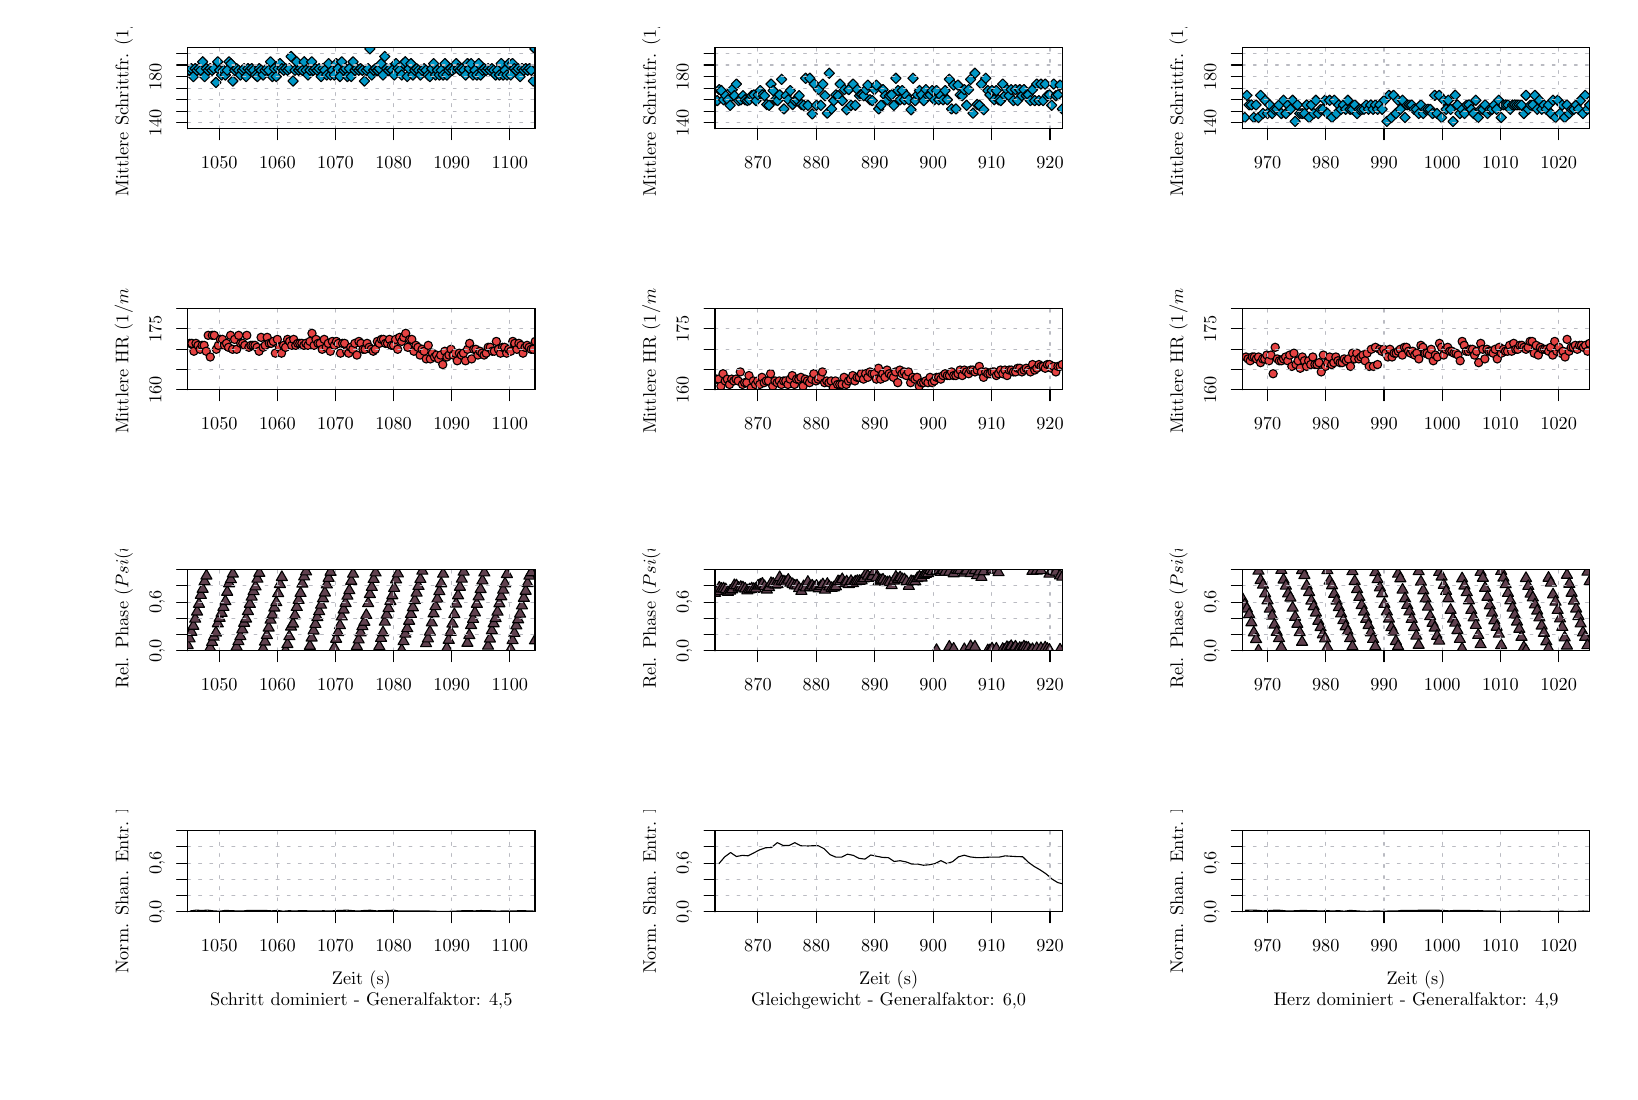
\begin{tikzpicture}[x=1pt,y=1pt]
\definecolor{fillColor}{RGB}{255,255,255}
\path[use as bounding box,fill=fillColor,fill opacity=0.00] (0,0) rectangle (571.66,377.25);
\begin{scope}
\path[clip] ( 57.82,340.75) rectangle (183.32,370.02);
\definecolor{drawColor}{RGB}{0,0,0}
\definecolor{fillColor}{RGB}{0,152,199}

\path[draw=drawColor,line width= 0.4pt,line join=round,line cap=round,fill=fillColor] ( 57.82,282.47) --
	( 59.68,284.33) --
	( 57.82,286.19) --
	( 55.95,284.33) --
	cycle;

\path[draw=drawColor,line width= 0.4pt,line join=round,line cap=round,fill=fillColor] ( 58.50,360.00) --
	( 60.36,361.86) --
	( 58.50,363.72) --
	( 56.63,361.86) --
	cycle;

\path[draw=drawColor,line width= 0.4pt,line join=round,line cap=round,fill=fillColor] ( 59.17,360.59) --
	( 61.03,362.45) --
	( 59.17,364.31) --
	( 57.31,362.45) --
	cycle;

\path[draw=drawColor,line width= 0.4pt,line join=round,line cap=round,fill=fillColor] ( 59.87,357.72) --
	( 61.73,359.58) --
	( 59.87,361.45) --
	( 58.01,359.58) --
	cycle;

\path[draw=drawColor,line width= 0.4pt,line join=round,line cap=round,fill=fillColor] ( 60.54,360.59) --
	( 62.40,362.45) --
	( 60.54,364.31) --
	( 58.68,362.45) --
	cycle;

\path[draw=drawColor,line width= 0.4pt,line join=round,line cap=round,fill=fillColor] ( 61.22,360.00) --
	( 63.08,361.86) --
	( 61.22,363.72) --
	( 59.36,361.86) --
	cycle;

\path[draw=drawColor,line width= 0.4pt,line join=round,line cap=round,fill=fillColor] ( 61.90,360.59) --
	( 63.76,362.45) --
	( 61.90,364.31) --
	( 60.04,362.45) --
	cycle;

\path[draw=drawColor,line width= 0.4pt,line join=round,line cap=round,fill=fillColor] ( 62.58,360.00) --
	( 64.44,361.86) --
	( 62.58,363.72) --
	( 60.72,361.86) --
	cycle;

\path[draw=drawColor,line width= 0.4pt,line join=round,line cap=round,fill=fillColor] ( 63.23,363.04) --
	( 65.09,364.90) --
	( 63.23,366.77) --
	( 61.37,364.90) --
	cycle;

\path[draw=drawColor,line width= 0.4pt,line join=round,line cap=round,fill=fillColor] ( 63.93,357.72) --
	( 65.79,359.58) --
	( 63.93,361.45) --
	( 62.07,359.58) --
	cycle;

\path[draw=drawColor,line width= 0.4pt,line join=round,line cap=round,fill=fillColor] ( 64.60,360.59) --
	( 66.47,362.45) --
	( 64.60,364.31) --
	( 62.74,362.45) --
	cycle;

\path[draw=drawColor,line width= 0.4pt,line join=round,line cap=round,fill=fillColor] ( 65.28,360.00) --
	( 67.14,361.86) --
	( 65.28,363.72) --
	( 63.42,361.86) --
	cycle;

\path[draw=drawColor,line width= 0.4pt,line join=round,line cap=round,fill=fillColor] ( 65.96,360.59) --
	( 67.82,362.45) --
	( 65.96,364.31) --
	( 64.10,362.45) --
	cycle;

\path[draw=drawColor,line width= 0.4pt,line join=round,line cap=round,fill=fillColor] ( 66.64,360.00) --
	( 68.50,361.86) --
	( 66.64,363.72) --
	( 64.78,361.86) --
	cycle;

\path[draw=drawColor,line width= 0.4pt,line join=round,line cap=round,fill=fillColor] ( 67.31,360.59) --
	( 69.17,362.45) --
	( 67.31,364.31) --
	( 65.45,362.45) --
	cycle;

\path[draw=drawColor,line width= 0.4pt,line join=round,line cap=round,fill=fillColor] ( 68.03,355.58) --
	( 69.89,357.44) --
	( 68.03,359.30) --
	( 66.17,357.44) --
	cycle;

\path[draw=drawColor,line width= 0.4pt,line join=round,line cap=round,fill=fillColor] ( 68.69,363.04) --
	( 70.55,364.90) --
	( 68.69,366.77) --
	( 66.82,364.90) --
	cycle;

\path[draw=drawColor,line width= 0.4pt,line join=round,line cap=round,fill=fillColor] ( 69.36,360.00) --
	( 71.23,361.86) --
	( 69.36,363.72) --
	( 67.50,361.86) --
	cycle;

\path[draw=drawColor,line width= 0.4pt,line join=round,line cap=round,fill=fillColor] ( 70.06,358.28) --
	( 71.92,360.15) --
	( 70.06,362.01) --
	( 68.20,360.15) --
	cycle;

\path[draw=drawColor,line width= 0.4pt,line join=round,line cap=round,fill=fillColor] ( 70.74,360.00) --
	( 72.60,361.86) --
	( 70.74,363.72) --
	( 68.88,361.86) --
	cycle;

\path[draw=drawColor,line width= 0.4pt,line join=round,line cap=round,fill=fillColor] ( 71.43,358.28) --
	( 73.29,360.15) --
	( 71.43,362.01) --
	( 69.57,360.15) --
	cycle;

\path[draw=drawColor,line width= 0.4pt,line join=round,line cap=round,fill=fillColor] ( 72.11,360.00) --
	( 73.97,361.86) --
	( 72.11,363.72) --
	( 70.25,361.86) --
	cycle;

\path[draw=drawColor,line width= 0.4pt,line join=round,line cap=round,fill=fillColor] ( 72.77,363.04) --
	( 74.63,364.91) --
	( 72.77,366.77) --
	( 70.90,364.91) --
	cycle;

\path[draw=drawColor,line width= 0.4pt,line join=round,line cap=round,fill=fillColor] ( 73.42,362.41) --
	( 75.29,364.27) --
	( 73.42,366.13) --
	( 71.56,364.27) --
	cycle;

\path[draw=drawColor,line width= 0.4pt,line join=round,line cap=round,fill=fillColor] ( 74.14,356.11) --
	( 76.00,357.97) --
	( 74.14,359.83) --
	( 72.28,357.97) --
	cycle;

\path[draw=drawColor,line width= 0.4pt,line join=round,line cap=round,fill=fillColor] ( 74.82,360.00) --
	( 76.68,361.86) --
	( 74.82,363.72) --
	( 72.96,361.86) --
	cycle;

\path[draw=drawColor,line width= 0.4pt,line join=round,line cap=round,fill=fillColor] ( 75.49,360.59) --
	( 77.35,362.45) --
	( 75.49,364.31) --
	( 73.63,362.45) --
	cycle;

\path[draw=drawColor,line width= 0.4pt,line join=round,line cap=round,fill=fillColor] ( 76.17,360.00) --
	( 78.03,361.86) --
	( 76.17,363.72) --
	( 74.31,361.86) --
	cycle;

\path[draw=drawColor,line width= 0.4pt,line join=round,line cap=round,fill=fillColor] ( 76.87,358.29) --
	( 78.73,360.15) --
	( 76.87,362.01) --
	( 75.01,360.15) --
	cycle;

\path[draw=drawColor,line width= 0.4pt,line join=round,line cap=round,fill=fillColor] ( 77.55,360.00) --
	( 79.41,361.86) --
	( 77.55,363.72) --
	( 75.69,361.86) --
	cycle;

\path[draw=drawColor,line width= 0.4pt,line join=round,line cap=round,fill=fillColor] ( 78.22,360.59) --
	( 80.08,362.45) --
	( 78.22,364.31) --
	( 76.36,362.45) --
	cycle;

\path[draw=drawColor,line width= 0.4pt,line join=round,line cap=round,fill=fillColor] ( 78.92,357.72) --
	( 80.78,359.58) --
	( 78.92,361.45) --
	( 77.06,359.58) --
	cycle;

\path[draw=drawColor,line width= 0.4pt,line join=round,line cap=round,fill=fillColor] ( 79.60,360.59) --
	( 81.46,362.45) --
	( 79.60,364.31) --
	( 77.73,362.45) --
	cycle;

\path[draw=drawColor,line width= 0.4pt,line join=round,line cap=round,fill=fillColor] ( 80.27,360.00) --
	( 82.14,361.86) --
	( 80.27,363.72) --
	( 78.41,361.86) --
	cycle;

\path[draw=drawColor,line width= 0.4pt,line join=round,line cap=round,fill=fillColor] ( 80.95,360.59) --
	( 82.81,362.45) --
	( 80.95,364.31) --
	( 79.09,362.45) --
	cycle;

\path[draw=drawColor,line width= 0.4pt,line join=round,line cap=round,fill=fillColor] ( 81.63,360.00) --
	( 83.49,361.86) --
	( 81.63,363.72) --
	( 79.77,361.86) --
	cycle;

\path[draw=drawColor,line width= 0.4pt,line join=round,line cap=round,fill=fillColor] ( 82.32,358.28) --
	( 84.18,360.15) --
	( 82.32,362.01) --
	( 80.46,360.15) --
	cycle;

\path[draw=drawColor,line width= 0.4pt,line join=round,line cap=round,fill=fillColor] ( 83.02,357.72) --
	( 84.88,359.58) --
	( 83.02,361.45) --
	( 81.16,359.58) --
	cycle;

\path[draw=drawColor,line width= 0.4pt,line join=round,line cap=round,fill=fillColor] ( 83.70,360.59) --
	( 85.56,362.45) --
	( 83.70,364.31) --
	( 81.84,362.45) --
	cycle;

\path[draw=drawColor,line width= 0.4pt,line join=round,line cap=round,fill=fillColor] ( 84.38,360.00) --
	( 86.24,361.86) --
	( 84.38,363.72) --
	( 82.51,361.86) --
	cycle;

\path[draw=drawColor,line width= 0.4pt,line join=round,line cap=round,fill=fillColor] ( 85.07,358.29) --
	( 86.93,360.15) --
	( 85.07,362.01) --
	( 83.21,360.15) --
	cycle;

\path[draw=drawColor,line width= 0.4pt,line join=round,line cap=round,fill=fillColor] ( 85.75,360.00) --
	( 87.61,361.86) --
	( 85.75,363.72) --
	( 83.89,361.86) --
	cycle;

\path[draw=drawColor,line width= 0.4pt,line join=round,line cap=round,fill=fillColor] ( 86.42,360.59) --
	( 88.29,362.45) --
	( 86.42,364.31) --
	( 84.56,362.45) --
	cycle;

\path[draw=drawColor,line width= 0.4pt,line join=round,line cap=round,fill=fillColor] ( 87.10,360.00) --
	( 88.96,361.86) --
	( 87.10,363.72) --
	( 85.24,361.86) --
	cycle;

\path[draw=drawColor,line width= 0.4pt,line join=round,line cap=round,fill=fillColor] ( 87.76,363.04) --
	( 89.62,364.91) --
	( 87.76,366.77) --
	( 85.90,364.91) --
	cycle;

\path[draw=drawColor,line width= 0.4pt,line join=round,line cap=round,fill=fillColor] ( 88.46,357.72) --
	( 90.32,359.58) --
	( 88.46,361.45) --
	( 86.60,359.58) --
	cycle;

\path[draw=drawColor,line width= 0.4pt,line join=round,line cap=round,fill=fillColor] ( 89.13,360.59) --
	( 90.99,362.45) --
	( 89.13,364.31) --
	( 87.27,362.45) --
	cycle;

\path[draw=drawColor,line width= 0.4pt,line join=round,line cap=round,fill=fillColor] ( 89.83,357.72) --
	( 91.69,359.58) --
	( 89.83,361.45) --
	( 87.97,359.58) --
	cycle;

\path[draw=drawColor,line width= 0.4pt,line join=round,line cap=round,fill=fillColor] ( 90.51,360.59) --
	( 92.37,362.45) --
	( 90.51,364.31) --
	( 88.64,362.45) --
	cycle;

\path[draw=drawColor,line width= 0.4pt,line join=round,line cap=round,fill=fillColor] ( 91.16,362.41) --
	( 93.03,364.27) --
	( 91.16,366.13) --
	( 89.30,364.27) --
	cycle;

\path[draw=drawColor,line width= 0.4pt,line join=round,line cap=round,fill=fillColor] ( 91.84,360.59) --
	( 93.70,362.45) --
	( 91.84,364.31) --
	( 89.98,362.45) --
	cycle;

\path[draw=drawColor,line width= 0.4pt,line join=round,line cap=round,fill=fillColor] ( 92.52,360.00) --
	( 94.38,361.86) --
	( 92.52,363.72) --
	( 90.66,361.86) --
	cycle;

\path[draw=drawColor,line width= 0.4pt,line join=round,line cap=round,fill=fillColor] ( 93.19,360.59) --
	( 95.05,362.45) --
	( 93.19,364.31) --
	( 91.33,362.45) --
	cycle;

\path[draw=drawColor,line width= 0.4pt,line join=round,line cap=round,fill=fillColor] ( 93.87,360.00) --
	( 95.73,361.86) --
	( 93.87,363.72) --
	( 92.01,361.86) --
	cycle;

\path[draw=drawColor,line width= 0.4pt,line join=round,line cap=round,fill=fillColor] ( 94.55,360.59) --
	( 96.41,362.45) --
	( 94.55,364.31) --
	( 92.68,362.45) --
	cycle;

\path[draw=drawColor,line width= 0.4pt,line join=round,line cap=round,fill=fillColor] ( 95.18,364.98) --
	( 97.04,366.84) --
	( 95.18,368.70) --
	( 93.32,366.84) --
	cycle;

\path[draw=drawColor,line width= 0.4pt,line join=round,line cap=round,fill=fillColor] ( 95.90,356.11) --
	( 97.76,357.97) --
	( 95.90,359.83) --
	( 94.04,357.97) --
	cycle;

\path[draw=drawColor,line width= 0.4pt,line join=round,line cap=round,fill=fillColor] ( 96.58,360.00) --
	( 98.44,361.86) --
	( 96.58,363.72) --
	( 94.72,361.86) --
	cycle;

\path[draw=drawColor,line width= 0.4pt,line join=round,line cap=round,fill=fillColor] ( 97.23,363.04) --
	( 99.09,364.90) --
	( 97.23,366.77) --
	( 95.37,364.90) --
	cycle;

\path[draw=drawColor,line width= 0.4pt,line join=round,line cap=round,fill=fillColor] ( 97.91,360.00) --
	( 99.77,361.86) --
	( 97.91,363.72) --
	( 96.05,361.86) --
	cycle;

\path[draw=drawColor,line width= 0.4pt,line join=round,line cap=round,fill=fillColor] ( 98.59,360.59) --
	(100.45,362.45) --
	( 98.59,364.31) --
	( 96.72,362.45) --
	cycle;

\path[draw=drawColor,line width= 0.4pt,line join=round,line cap=round,fill=fillColor] ( 99.26,360.00) --
	(101.13,361.86) --
	( 99.26,363.72) --
	( 97.40,361.86) --
	cycle;

\path[draw=drawColor,line width= 0.4pt,line join=round,line cap=round,fill=fillColor] ( 99.92,363.04) --
	(101.78,364.90) --
	( 99.92,366.77) --
	( 98.06,364.90) --
	cycle;

\path[draw=drawColor,line width= 0.4pt,line join=round,line cap=round,fill=fillColor] (100.60,360.00) --
	(102.46,361.86) --
	(100.60,363.72) --
	( 98.74,361.86) --
	cycle;

\path[draw=drawColor,line width= 0.4pt,line join=round,line cap=round,fill=fillColor] (101.29,358.28) --
	(103.15,360.15) --
	(101.29,362.01) --
	( 99.43,360.15) --
	cycle;

\path[draw=drawColor,line width= 0.4pt,line join=round,line cap=round,fill=fillColor] (101.97,360.00) --
	(103.83,361.86) --
	(101.97,363.72) --
	(100.11,361.86) --
	cycle;

\path[draw=drawColor,line width= 0.4pt,line join=round,line cap=round,fill=fillColor] (102.63,363.04) --
	(104.49,364.91) --
	(102.63,366.77) --
	(100.76,364.91) --
	cycle;

\path[draw=drawColor,line width= 0.4pt,line join=round,line cap=round,fill=fillColor] (103.30,360.00) --
	(105.17,361.86) --
	(103.30,363.72) --
	(101.44,361.86) --
	cycle;

\path[draw=drawColor,line width= 0.4pt,line join=round,line cap=round,fill=fillColor] (103.98,360.59) --
	(105.84,362.45) --
	(103.98,364.31) --
	(102.12,362.45) --
	cycle;

\path[draw=drawColor,line width= 0.4pt,line join=round,line cap=round,fill=fillColor] (104.66,360.00) --
	(106.52,361.86) --
	(104.66,363.72) --
	(102.80,361.86) --
	cycle;

\path[draw=drawColor,line width= 0.4pt,line join=round,line cap=round,fill=fillColor] (105.33,360.59) --
	(107.19,362.45) --
	(105.33,364.31) --
	(103.47,362.45) --
	cycle;

\path[draw=drawColor,line width= 0.4pt,line join=round,line cap=round,fill=fillColor] (106.03,357.72) --
	(107.89,359.58) --
	(106.03,361.45) --
	(104.17,359.58) --
	cycle;

\path[draw=drawColor,line width= 0.4pt,line join=round,line cap=round,fill=fillColor] (106.71,360.59) --
	(108.57,362.45) --
	(106.71,364.31) --
	(104.84,362.45) --
	cycle;

\path[draw=drawColor,line width= 0.4pt,line join=round,line cap=round,fill=fillColor] (107.39,360.00) --
	(109.25,361.86) --
	(107.39,363.72) --
	(105.52,361.86) --
	cycle;

\path[draw=drawColor,line width= 0.4pt,line join=round,line cap=round,fill=fillColor] (108.08,358.28) --
	(109.94,360.15) --
	(108.08,362.01) --
	(106.22,360.15) --
	cycle;

\path[draw=drawColor,line width= 0.4pt,line join=round,line cap=round,fill=fillColor] (108.74,362.41) --
	(110.60,364.27) --
	(108.74,366.13) --
	(106.88,364.27) --
	cycle;

\path[draw=drawColor,line width= 0.4pt,line join=round,line cap=round,fill=fillColor] (109.43,358.28) --
	(111.29,360.15) --
	(109.43,362.01) --
	(107.57,360.15) --
	cycle;

\path[draw=drawColor,line width= 0.4pt,line join=round,line cap=round,fill=fillColor] (110.11,360.00) --
	(111.97,361.86) --
	(110.11,363.72) --
	(108.25,361.86) --
	cycle;

\path[draw=drawColor,line width= 0.4pt,line join=round,line cap=round,fill=fillColor] (110.81,358.28) --
	(112.67,360.15) --
	(110.81,362.01) --
	(108.95,360.15) --
	cycle;

\path[draw=drawColor,line width= 0.4pt,line join=round,line cap=round,fill=fillColor] (111.47,362.41) --
	(113.33,364.27) --
	(111.47,366.13) --
	(109.61,364.27) --
	cycle;

\path[draw=drawColor,line width= 0.4pt,line join=round,line cap=round,fill=fillColor] (112.14,360.59) --
	(114.00,362.45) --
	(112.14,364.31) --
	(110.28,362.45) --
	cycle;

\path[draw=drawColor,line width= 0.4pt,line join=round,line cap=round,fill=fillColor] (112.84,357.72) --
	(114.70,359.58) --
	(112.84,361.45) --
	(110.98,359.58) --
	cycle;

\path[draw=drawColor,line width= 0.4pt,line join=round,line cap=round,fill=fillColor] (113.49,363.04) --
	(115.36,364.90) --
	(113.49,366.77) --
	(111.63,364.90) --
	cycle;

\path[draw=drawColor,line width= 0.4pt,line join=round,line cap=round,fill=fillColor] (114.17,360.00) --
	(116.03,361.86) --
	(114.17,363.72) --
	(112.31,361.86) --
	cycle;

\path[draw=drawColor,line width= 0.4pt,line join=round,line cap=round,fill=fillColor] (114.85,360.59) --
	(116.71,362.45) --
	(114.85,364.31) --
	(112.99,362.45) --
	cycle;

\path[draw=drawColor,line width= 0.4pt,line join=round,line cap=round,fill=fillColor] (115.55,357.72) --
	(117.41,359.58) --
	(115.55,361.45) --
	(113.69,359.58) --
	cycle;

\path[draw=drawColor,line width= 0.4pt,line join=round,line cap=round,fill=fillColor] (116.22,360.59) --
	(118.08,362.45) --
	(116.22,364.31) --
	(114.36,362.45) --
	cycle;

\path[draw=drawColor,line width= 0.4pt,line join=round,line cap=round,fill=fillColor] (116.92,357.72) --
	(118.78,359.58) --
	(116.92,361.45) --
	(115.06,359.58) --
	cycle;

\path[draw=drawColor,line width= 0.4pt,line join=round,line cap=round,fill=fillColor] (117.58,363.04) --
	(119.44,364.90) --
	(117.58,366.77) --
	(115.71,364.90) --
	cycle;

\path[draw=drawColor,line width= 0.4pt,line join=round,line cap=round,fill=fillColor] (118.25,360.00) --
	(120.12,361.86) --
	(118.25,363.72) --
	(116.39,361.86) --
	cycle;

\path[draw=drawColor,line width= 0.4pt,line join=round,line cap=round,fill=fillColor] (118.93,360.59) --
	(120.79,362.45) --
	(118.93,364.31) --
	(117.07,362.45) --
	cycle;

\path[draw=drawColor,line width= 0.4pt,line join=round,line cap=round,fill=fillColor] (119.61,360.00) --
	(121.47,361.86) --
	(119.61,363.72) --
	(117.75,361.86) --
	cycle;

\path[draw=drawColor,line width= 0.4pt,line join=round,line cap=round,fill=fillColor] (120.28,360.59) --
	(122.14,362.45) --
	(120.28,364.31) --
	(118.42,362.45) --
	cycle;

\path[draw=drawColor,line width= 0.4pt,line join=round,line cap=round,fill=fillColor] (120.96,360.00) --
	(122.82,361.86) --
	(120.96,363.72) --
	(119.10,361.86) --
	cycle;

\path[draw=drawColor,line width= 0.4pt,line join=round,line cap=round,fill=fillColor] (121.68,356.11) --
	(123.54,357.97) --
	(121.68,359.83) --
	(119.82,357.97) --
	cycle;

\path[draw=drawColor,line width= 0.4pt,line join=round,line cap=round,fill=fillColor] (122.36,360.00) --
	(124.22,361.86) --
	(122.36,363.72) --
	(120.49,361.86) --
	cycle;

\path[draw=drawColor,line width= 0.4pt,line join=round,line cap=round,fill=fillColor] (123.03,360.59) --
	(124.89,362.45) --
	(123.03,364.31) --
	(121.17,362.45) --
	cycle;

\path[draw=drawColor,line width= 0.4pt,line join=round,line cap=round,fill=fillColor] (123.65,367.72) --
	(125.51,369.58) --
	(123.65,371.44) --
	(121.79,369.58) --
	cycle;

\path[draw=drawColor,line width= 0.4pt,line join=round,line cap=round,fill=fillColor] (124.34,358.28) --
	(126.20,360.15) --
	(124.34,362.01) --
	(122.48,360.15) --
	cycle;

\path[draw=drawColor,line width= 0.4pt,line join=round,line cap=round,fill=fillColor] (125.02,360.00) --
	(126.88,361.86) --
	(125.02,363.72) --
	(123.16,361.86) --
	cycle;

\path[draw=drawColor,line width= 0.4pt,line join=round,line cap=round,fill=fillColor] (125.70,360.59) --
	(127.56,362.45) --
	(125.70,364.31) --
	(123.83,362.45) --
	cycle;

\path[draw=drawColor,line width= 0.4pt,line join=round,line cap=round,fill=fillColor] (126.38,360.00) --
	(128.24,361.86) --
	(126.38,363.72) --
	(124.51,361.86) --
	cycle;

\path[draw=drawColor,line width= 0.4pt,line join=round,line cap=round,fill=fillColor] (127.05,360.59) --
	(128.91,362.45) --
	(127.05,364.31) --
	(125.19,362.45) --
	cycle;

\path[draw=drawColor,line width= 0.4pt,line join=round,line cap=round,fill=fillColor] (127.71,362.41) --
	(129.57,364.27) --
	(127.71,366.13) --
	(125.85,364.27) --
	cycle;

\path[draw=drawColor,line width= 0.4pt,line join=round,line cap=round,fill=fillColor] (128.40,358.28) --
	(130.26,360.15) --
	(128.40,362.01) --
	(126.54,360.15) --
	cycle;

\path[draw=drawColor,line width= 0.4pt,line join=round,line cap=round,fill=fillColor] (129.04,364.98) --
	(130.90,366.84) --
	(129.04,368.70) --
	(127.18,366.84) --
	cycle;

\path[draw=drawColor,line width= 0.4pt,line join=round,line cap=round,fill=fillColor] (129.72,360.59) --
	(131.58,362.45) --
	(129.72,364.31) --
	(127.85,362.45) --
	cycle;

\path[draw=drawColor,line width= 0.4pt,line join=round,line cap=round,fill=fillColor] (130.39,360.00) --
	(132.26,361.86) --
	(130.39,363.72) --
	(128.53,361.86) --
	cycle;

\path[draw=drawColor,line width= 0.4pt,line join=round,line cap=round,fill=fillColor] (131.07,360.59) --
	(132.93,362.45) --
	(131.07,364.31) --
	(129.21,362.45) --
	cycle;

\path[draw=drawColor,line width= 0.4pt,line join=round,line cap=round,fill=fillColor] (131.75,360.00) --
	(133.61,361.86) --
	(131.75,363.72) --
	(129.89,361.86) --
	cycle;

\path[draw=drawColor,line width= 0.4pt,line join=round,line cap=round,fill=fillColor] (132.44,358.28) --
	(134.30,360.15) --
	(132.44,362.01) --
	(130.58,360.15) --
	cycle;

\path[draw=drawColor,line width= 0.4pt,line join=round,line cap=round,fill=fillColor] (133.10,362.41) --
	(134.96,364.27) --
	(133.10,366.13) --
	(131.24,364.27) --
	cycle;

\path[draw=drawColor,line width= 0.4pt,line join=round,line cap=round,fill=fillColor] (133.78,360.59) --
	(135.64,362.45) --
	(133.78,364.31) --
	(131.91,362.45) --
	cycle;

\path[draw=drawColor,line width= 0.4pt,line join=round,line cap=round,fill=fillColor] (134.46,360.00) --
	(136.32,361.86) --
	(134.46,363.72) --
	(132.59,361.86) --
	cycle;

\path[draw=drawColor,line width= 0.4pt,line join=round,line cap=round,fill=fillColor] (135.15,358.28) --
	(137.01,360.15) --
	(135.15,362.01) --
	(133.29,360.15) --
	cycle;

\path[draw=drawColor,line width= 0.4pt,line join=round,line cap=round,fill=fillColor] (135.81,362.41) --
	(137.67,364.27) --
	(135.81,366.13) --
	(133.95,364.27) --
	cycle;

\path[draw=drawColor,line width= 0.4pt,line join=round,line cap=round,fill=fillColor] (136.46,363.04) --
	(138.32,364.90) --
	(136.46,366.77) --
	(134.60,364.90) --
	cycle;

\path[draw=drawColor,line width= 0.4pt,line join=round,line cap=round,fill=fillColor] (137.16,357.72) --
	(139.02,359.58) --
	(137.16,361.45) --
	(135.30,359.58) --
	cycle;

\path[draw=drawColor,line width= 0.4pt,line join=round,line cap=round,fill=fillColor] (137.84,360.59) --
	(139.70,362.45) --
	(137.84,364.31) --
	(135.98,362.45) --
	cycle;

\path[draw=drawColor,line width= 0.4pt,line join=round,line cap=round,fill=fillColor] (138.50,362.41) --
	(140.36,364.27) --
	(138.50,366.13) --
	(136.63,364.27) --
	cycle;

\path[draw=drawColor,line width= 0.4pt,line join=round,line cap=round,fill=fillColor] (139.19,358.28) --
	(141.05,360.15) --
	(139.19,362.01) --
	(137.33,360.15) --
	cycle;

\path[draw=drawColor,line width= 0.4pt,line join=round,line cap=round,fill=fillColor] (139.87,360.00) --
	(141.73,361.86) --
	(139.87,363.72) --
	(138.01,361.86) --
	cycle;

\path[draw=drawColor,line width= 0.4pt,line join=round,line cap=round,fill=fillColor] (140.54,360.59) --
	(142.40,362.45) --
	(140.54,364.31) --
	(138.68,362.45) --
	cycle;

\path[draw=drawColor,line width= 0.4pt,line join=round,line cap=round,fill=fillColor] (141.22,360.00) --
	(143.08,361.86) --
	(141.22,363.72) --
	(139.36,361.86) --
	cycle;

\path[draw=drawColor,line width= 0.4pt,line join=round,line cap=round,fill=fillColor] (141.92,358.28) --
	(143.78,360.15) --
	(141.92,362.01) --
	(140.06,360.15) --
	cycle;

\path[draw=drawColor,line width= 0.4pt,line join=round,line cap=round,fill=fillColor] (142.60,360.00) --
	(144.46,361.86) --
	(142.60,363.72) --
	(140.74,361.86) --
	cycle;

\path[draw=drawColor,line width= 0.4pt,line join=round,line cap=round,fill=fillColor] (143.27,360.59) --
	(145.13,362.45) --
	(143.27,364.31) --
	(141.41,362.45) --
	cycle;

\path[draw=drawColor,line width= 0.4pt,line join=round,line cap=round,fill=fillColor] (143.95,360.00) --
	(145.81,361.86) --
	(143.95,363.72) --
	(142.09,361.86) --
	cycle;

\path[draw=drawColor,line width= 0.4pt,line join=round,line cap=round,fill=fillColor] (144.65,358.28) --
	(146.51,360.15) --
	(144.65,362.01) --
	(142.78,360.15) --
	cycle;

\path[draw=drawColor,line width= 0.4pt,line join=round,line cap=round,fill=fillColor] (145.34,357.72) --
	(147.21,359.58) --
	(145.34,361.45) --
	(143.48,359.58) --
	cycle;

\path[draw=drawColor,line width= 0.4pt,line join=round,line cap=round,fill=fillColor] (146.02,360.59) --
	(147.88,362.45) --
	(146.02,364.31) --
	(144.16,362.45) --
	cycle;

\path[draw=drawColor,line width= 0.4pt,line join=round,line cap=round,fill=fillColor] (146.68,362.41) --
	(148.54,364.27) --
	(146.68,366.13) --
	(144.82,364.27) --
	cycle;

\path[draw=drawColor,line width= 0.4pt,line join=round,line cap=round,fill=fillColor] (147.37,358.28) --
	(149.23,360.15) --
	(147.37,362.01) --
	(145.51,360.15) --
	cycle;

\path[draw=drawColor,line width= 0.4pt,line join=round,line cap=round,fill=fillColor] (148.05,360.00) --
	(149.91,361.86) --
	(148.05,363.72) --
	(146.19,361.86) --
	cycle;

\path[draw=drawColor,line width= 0.4pt,line join=round,line cap=round,fill=fillColor] (148.75,358.28) --
	(150.61,360.15) --
	(148.75,362.01) --
	(146.89,360.15) --
	cycle;

\path[draw=drawColor,line width= 0.4pt,line join=round,line cap=round,fill=fillColor] (149.43,360.00) --
	(151.29,361.86) --
	(149.43,363.72) --
	(147.56,361.86) --
	cycle;

\path[draw=drawColor,line width= 0.4pt,line join=round,line cap=round,fill=fillColor] (150.12,358.28) --
	(151.98,360.15) --
	(150.12,362.01) --
	(148.26,360.15) --
	cycle;

\path[draw=drawColor,line width= 0.4pt,line join=round,line cap=round,fill=fillColor] (150.78,362.41) --
	(152.64,364.27) --
	(150.78,366.13) --
	(148.92,364.27) --
	cycle;

\path[draw=drawColor,line width= 0.4pt,line join=round,line cap=round,fill=fillColor] (151.47,358.28) --
	(153.34,360.15) --
	(151.47,362.01) --
	(149.61,360.15) --
	cycle;

\path[draw=drawColor,line width= 0.4pt,line join=round,line cap=round,fill=fillColor] (152.15,360.00) --
	(154.01,361.86) --
	(152.15,363.72) --
	(150.29,361.86) --
	cycle;

\path[draw=drawColor,line width= 0.4pt,line join=round,line cap=round,fill=fillColor] (152.83,360.59) --
	(154.69,362.45) --
	(152.83,364.31) --
	(150.97,362.45) --
	cycle;

\path[draw=drawColor,line width= 0.4pt,line join=round,line cap=round,fill=fillColor] (153.51,360.00) --
	(155.37,361.86) --
	(153.51,363.72) --
	(151.65,361.86) --
	cycle;

\path[draw=drawColor,line width= 0.4pt,line join=round,line cap=round,fill=fillColor] (154.18,360.59) --
	(156.04,362.45) --
	(154.18,364.31) --
	(152.32,362.45) --
	cycle;

\path[draw=drawColor,line width= 0.4pt,line join=round,line cap=round,fill=fillColor] (154.84,362.41) --
	(156.70,364.27) --
	(154.84,366.13) --
	(152.98,364.27) --
	cycle;

\path[draw=drawColor,line width= 0.4pt,line join=round,line cap=round,fill=fillColor] (155.51,360.59) --
	(157.38,362.45) --
	(155.51,364.31) --
	(153.65,362.45) --
	cycle;

\path[draw=drawColor,line width= 0.4pt,line join=round,line cap=round,fill=fillColor] (156.19,360.00) --
	(158.05,361.86) --
	(156.19,363.72) --
	(154.33,361.86) --
	cycle;

\path[draw=drawColor,line width= 0.4pt,line join=round,line cap=round,fill=fillColor] (156.87,360.59) --
	(158.73,362.45) --
	(156.87,364.31) --
	(155.01,362.45) --
	cycle;

\path[draw=drawColor,line width= 0.4pt,line join=round,line cap=round,fill=fillColor] (157.55,360.00) --
	(159.41,361.86) --
	(157.55,363.72) --
	(155.69,361.86) --
	cycle;

\path[draw=drawColor,line width= 0.4pt,line join=round,line cap=round,fill=fillColor] (158.24,358.29) --
	(160.10,360.15) --
	(158.24,362.01) --
	(156.38,360.15) --
	cycle;

\path[draw=drawColor,line width= 0.4pt,line join=round,line cap=round,fill=fillColor] (158.90,362.41) --
	(160.76,364.27) --
	(158.90,366.13) --
	(157.04,364.27) --
	cycle;

\path[draw=drawColor,line width= 0.4pt,line join=round,line cap=round,fill=fillColor] (159.57,360.59) --
	(161.44,362.45) --
	(159.57,364.31) --
	(157.71,362.45) --
	cycle;

\path[draw=drawColor,line width= 0.4pt,line join=round,line cap=round,fill=fillColor] (160.23,362.41) --
	(162.09,364.27) --
	(160.23,366.13) --
	(158.37,364.27) --
	cycle;

\path[draw=drawColor,line width= 0.4pt,line join=round,line cap=round,fill=fillColor] (160.93,358.28) --
	(162.79,360.15) --
	(160.93,362.01) --
	(159.07,360.15) --
	cycle;

\path[draw=drawColor,line width= 0.4pt,line join=round,line cap=round,fill=fillColor] (161.61,360.00) --
	(163.47,361.86) --
	(161.61,363.72) --
	(159.75,361.86) --
	cycle;

\path[draw=drawColor,line width= 0.4pt,line join=round,line cap=round,fill=fillColor] (162.30,358.28) --
	(164.16,360.15) --
	(162.30,362.01) --
	(160.44,360.15) --
	cycle;

\path[draw=drawColor,line width= 0.4pt,line join=round,line cap=round,fill=fillColor] (162.96,362.41) --
	(164.82,364.27) --
	(162.96,366.13) --
	(161.10,364.27) --
	cycle;

\path[draw=drawColor,line width= 0.4pt,line join=round,line cap=round,fill=fillColor] (163.66,358.28) --
	(165.52,360.15) --
	(163.66,362.01) --
	(161.79,360.15) --
	cycle;

\path[draw=drawColor,line width= 0.4pt,line join=round,line cap=round,fill=fillColor] (164.33,360.00) --
	(166.20,361.86) --
	(164.33,363.72) --
	(162.47,361.86) --
	cycle;

\path[draw=drawColor,line width= 0.4pt,line join=round,line cap=round,fill=fillColor] (165.01,360.59) --
	(166.87,362.45) --
	(165.01,364.31) --
	(163.15,362.45) --
	cycle;

\path[draw=drawColor,line width= 0.4pt,line join=round,line cap=round,fill=fillColor] (165.69,360.00) --
	(167.55,361.86) --
	(165.69,363.72) --
	(163.83,361.86) --
	cycle;

\path[draw=drawColor,line width= 0.4pt,line join=round,line cap=round,fill=fillColor] (166.36,360.59) --
	(168.22,362.45) --
	(166.36,364.31) --
	(164.50,362.45) --
	cycle;

\path[draw=drawColor,line width= 0.4pt,line join=round,line cap=round,fill=fillColor] (167.04,360.00) --
	(168.90,361.86) --
	(167.04,363.72) --
	(165.18,361.86) --
	cycle;

\path[draw=drawColor,line width= 0.4pt,line join=round,line cap=round,fill=fillColor] (167.72,360.59) --
	(169.58,362.45) --
	(167.72,364.31) --
	(165.85,362.45) --
	cycle;

\path[draw=drawColor,line width= 0.4pt,line join=round,line cap=round,fill=fillColor] (168.40,360.00) --
	(170.26,361.86) --
	(168.40,363.72) --
	(166.53,361.86) --
	cycle;

\path[draw=drawColor,line width= 0.4pt,line join=round,line cap=round,fill=fillColor] (169.09,358.28) --
	(170.95,360.15) --
	(169.09,362.01) --
	(167.23,360.15) --
	cycle;

\path[draw=drawColor,line width= 0.4pt,line join=round,line cap=round,fill=fillColor] (169.77,360.00) --
	(171.63,361.86) --
	(169.77,363.72) --
	(167.91,361.86) --
	cycle;

\path[draw=drawColor,line width= 0.4pt,line join=round,line cap=round,fill=fillColor] (170.46,358.28) --
	(172.33,360.15) --
	(170.46,362.01) --
	(168.60,360.15) --
	cycle;

\path[draw=drawColor,line width= 0.4pt,line join=round,line cap=round,fill=fillColor] (171.12,362.41) --
	(172.98,364.27) --
	(171.12,366.13) --
	(169.26,364.27) --
	cycle;

\path[draw=drawColor,line width= 0.4pt,line join=round,line cap=round,fill=fillColor] (171.82,358.28) --
	(173.68,360.15) --
	(171.82,362.01) --
	(169.96,360.15) --
	cycle;

\path[draw=drawColor,line width= 0.4pt,line join=round,line cap=round,fill=fillColor] (172.50,360.00) --
	(174.36,361.86) --
	(172.50,363.72) --
	(170.64,361.86) --
	cycle;

\path[draw=drawColor,line width= 0.4pt,line join=round,line cap=round,fill=fillColor] (173.19,358.28) --
	(175.05,360.15) --
	(173.19,362.01) --
	(171.33,360.15) --
	cycle;

\path[draw=drawColor,line width= 0.4pt,line join=round,line cap=round,fill=fillColor] (173.85,362.41) --
	(175.71,364.27) --
	(173.85,366.13) --
	(171.99,364.27) --
	cycle;

\path[draw=drawColor,line width= 0.4pt,line join=round,line cap=round,fill=fillColor] (174.55,358.28) --
	(176.41,360.15) --
	(174.55,362.01) --
	(172.68,360.15) --
	cycle;

\path[draw=drawColor,line width= 0.4pt,line join=round,line cap=round,fill=fillColor] (175.20,362.41) --
	(177.07,364.27) --
	(175.20,366.13) --
	(173.34,364.27) --
	cycle;

\path[draw=drawColor,line width= 0.4pt,line join=round,line cap=round,fill=fillColor] (175.88,360.59) --
	(177.74,362.45) --
	(175.88,364.31) --
	(174.02,362.45) --
	cycle;

\path[draw=drawColor,line width= 0.4pt,line join=round,line cap=round,fill=fillColor] (176.56,360.00) --
	(178.42,361.86) --
	(176.56,363.72) --
	(174.70,361.86) --
	cycle;

\path[draw=drawColor,line width= 0.4pt,line join=round,line cap=round,fill=fillColor] (177.23,360.59) --
	(179.09,362.45) --
	(177.23,364.31) --
	(175.37,362.45) --
	cycle;

\path[draw=drawColor,line width= 0.4pt,line join=round,line cap=round,fill=fillColor] (177.93,357.72) --
	(179.79,359.58) --
	(177.93,361.45) --
	(176.07,359.58) --
	cycle;

\path[draw=drawColor,line width= 0.4pt,line join=round,line cap=round,fill=fillColor] (178.61,360.59) --
	(180.47,362.45) --
	(178.61,364.31) --
	(176.74,362.45) --
	cycle;

\path[draw=drawColor,line width= 0.4pt,line join=round,line cap=round,fill=fillColor] (179.28,360.00) --
	(181.15,361.86) --
	(179.28,363.72) --
	(177.42,361.86) --
	cycle;

\path[draw=drawColor,line width= 0.4pt,line join=round,line cap=round,fill=fillColor] (179.96,360.59) --
	(181.82,362.45) --
	(179.96,364.31) --
	(178.10,362.45) --
	cycle;

\path[draw=drawColor,line width= 0.4pt,line join=round,line cap=round,fill=fillColor] (180.64,360.00) --
	(182.50,361.86) --
	(180.64,363.72) --
	(178.78,361.86) --
	cycle;

\path[draw=drawColor,line width= 0.4pt,line join=round,line cap=round,fill=fillColor] (181.31,360.59) --
	(183.17,362.45) --
	(181.31,364.31) --
	(179.45,362.45) --
	cycle;

\path[draw=drawColor,line width= 0.4pt,line join=round,line cap=round,fill=fillColor] (181.99,360.00) --
	(183.85,361.86) --
	(181.99,363.72) --
	(180.13,361.86) --
	cycle;

\path[draw=drawColor,line width= 0.4pt,line join=round,line cap=round,fill=fillColor] (182.71,356.11) --
	(184.57,357.97) --
	(182.71,359.83) --
	(180.85,357.97) --
	cycle;

\path[draw=drawColor,line width= 0.4pt,line join=round,line cap=round,fill=fillColor] (183.32,367.72) --
	(185.19,369.58) --
	(183.32,371.44) --
	(181.46,369.58) --
	cycle;
\end{scope}
\begin{scope}
\path[clip] (  0.00,  0.00) rectangle (571.66,377.25);
\definecolor{drawColor}{RGB}{0,0,0}

\path[draw=drawColor,line width= 0.4pt,line join=round,line cap=round] ( 69.23,340.75) -- (174.23,340.75);

\path[draw=drawColor,line width= 0.4pt,line join=round,line cap=round] ( 69.23,340.75) -- ( 69.23,336.79);

\path[draw=drawColor,line width= 0.4pt,line join=round,line cap=round] ( 90.23,340.75) -- ( 90.23,336.79);

\path[draw=drawColor,line width= 0.4pt,line join=round,line cap=round] (111.23,340.75) -- (111.23,336.79);

\path[draw=drawColor,line width= 0.4pt,line join=round,line cap=round] (132.23,340.75) -- (132.23,336.79);

\path[draw=drawColor,line width= 0.4pt,line join=round,line cap=round] (153.23,340.75) -- (153.23,336.79);

\path[draw=drawColor,line width= 0.4pt,line join=round,line cap=round] (174.23,340.75) -- (174.23,336.79);

\node[text=drawColor,anchor=base,inner sep=0pt, outer sep=0pt, scale=  0.66] at ( 69.23,326.50) {1050};

\node[text=drawColor,anchor=base,inner sep=0pt, outer sep=0pt, scale=  0.66] at ( 90.23,326.50) {1060};

\node[text=drawColor,anchor=base,inner sep=0pt, outer sep=0pt, scale=  0.66] at (111.23,326.50) {1070};

\node[text=drawColor,anchor=base,inner sep=0pt, outer sep=0pt, scale=  0.66] at (132.23,326.50) {1080};

\node[text=drawColor,anchor=base,inner sep=0pt, outer sep=0pt, scale=  0.66] at (153.23,326.50) {1090};

\node[text=drawColor,anchor=base,inner sep=0pt, outer sep=0pt, scale=  0.66] at (174.23,326.50) {1100};

\path[draw=drawColor,line width= 0.4pt,line join=round,line cap=round] ( 57.82,342.84) -- ( 57.82,367.93);

\path[draw=drawColor,line width= 0.4pt,line join=round,line cap=round] ( 57.82,342.84) -- ( 53.86,342.84);

\path[draw=drawColor,line width= 0.4pt,line join=round,line cap=round] ( 57.82,347.03) -- ( 53.86,347.03);

\path[draw=drawColor,line width= 0.4pt,line join=round,line cap=round] ( 57.82,351.21) -- ( 53.86,351.21);

\path[draw=drawColor,line width= 0.4pt,line join=round,line cap=round] ( 57.82,355.39) -- ( 53.86,355.39);

\path[draw=drawColor,line width= 0.4pt,line join=round,line cap=round] ( 57.82,359.57) -- ( 53.86,359.57);

\path[draw=drawColor,line width= 0.4pt,line join=round,line cap=round] ( 57.82,363.75) -- ( 53.86,363.75);

\path[draw=drawColor,line width= 0.4pt,line join=round,line cap=round] ( 57.82,367.93) -- ( 53.86,367.93);

\node[text=drawColor,rotate= 90.00,anchor=base,inner sep=0pt, outer sep=0pt, scale=  0.66] at ( 48.31,342.84) {140};

\node[text=drawColor,rotate= 90.00,anchor=base,inner sep=0pt, outer sep=0pt, scale=  0.66] at ( 48.31,359.57) {180};

\path[draw=drawColor,line width= 0.4pt,line join=round,line cap=round] ( 57.82,340.75) --
	(183.32,340.75) --
	(183.32,370.02) --
	( 57.82,370.02) --
	( 57.82,340.75);
\end{scope}
\begin{scope}
\path[clip] (  0.00,282.94) rectangle (190.55,377.25);
\definecolor{drawColor}{RGB}{0,0,0}

\node[text=drawColor,rotate= 90.00,anchor=base,inner sep=0pt, outer sep=0pt, scale=  0.66] at ( 36.43,355.39) {Mittlere Schrittfr. ($1/min$)};
\end{scope}
\begin{scope}
\path[clip] ( 57.82,340.75) rectangle (183.32,370.02);
\definecolor{drawColor}{RGB}{186,187,194}

\path[draw=drawColor,line width= 0.4pt,dash pattern=on 1pt off 3pt ,line join=round,line cap=round] ( 69.23,340.75) -- ( 69.23,370.02);

\path[draw=drawColor,line width= 0.4pt,dash pattern=on 1pt off 3pt ,line join=round,line cap=round] ( 90.23,340.75) -- ( 90.23,370.02);

\path[draw=drawColor,line width= 0.4pt,dash pattern=on 1pt off 3pt ,line join=round,line cap=round] (111.23,340.75) -- (111.23,370.02);

\path[draw=drawColor,line width= 0.4pt,dash pattern=on 1pt off 3pt ,line join=round,line cap=round] (132.23,340.75) -- (132.23,370.02);

\path[draw=drawColor,line width= 0.4pt,dash pattern=on 1pt off 3pt ,line join=round,line cap=round] (153.23,340.75) -- (153.23,370.02);

\path[draw=drawColor,line width= 0.4pt,dash pattern=on 1pt off 3pt ,line join=round,line cap=round] (174.23,340.75) -- (174.23,370.02);

\path[draw=drawColor,line width= 0.4pt,dash pattern=on 1pt off 3pt ,line join=round,line cap=round] ( 57.82,342.84) -- (183.32,342.84);

\path[draw=drawColor,line width= 0.4pt,dash pattern=on 1pt off 3pt ,line join=round,line cap=round] ( 57.82,347.03) -- (183.32,347.03);

\path[draw=drawColor,line width= 0.4pt,dash pattern=on 1pt off 3pt ,line join=round,line cap=round] ( 57.82,351.21) -- (183.32,351.21);

\path[draw=drawColor,line width= 0.4pt,dash pattern=on 1pt off 3pt ,line join=round,line cap=round] ( 57.82,355.39) -- (183.32,355.39);

\path[draw=drawColor,line width= 0.4pt,dash pattern=on 1pt off 3pt ,line join=round,line cap=round] ( 57.82,359.57) -- (183.32,359.57);

\path[draw=drawColor,line width= 0.4pt,dash pattern=on 1pt off 3pt ,line join=round,line cap=round] ( 57.82,363.75) -- (183.32,363.75);

\path[draw=drawColor,line width= 0.4pt,dash pattern=on 1pt off 3pt ,line join=round,line cap=round] ( 57.82,367.93) -- (183.32,367.93);
\end{scope}
\begin{scope}
\path[clip] (  0.00,  0.00) rectangle (571.66,377.25);
\definecolor{drawColor}{RGB}{0,0,0}

\path[draw=drawColor,line width= 0.4pt,line join=round,line cap=round] ( 57.82,340.75) --
	(183.32,340.75) --
	(183.32,370.02) --
	( 57.82,370.02) --
	( 57.82,340.75);
\end{scope}
\begin{scope}
\path[clip] ( 57.82,246.44) rectangle (183.32,275.71);
\definecolor{drawColor}{RGB}{0,0,0}
\definecolor{fillColor}{RGB}{229,66,66}

\path[draw=drawColor,line width= 0.4pt,line join=round,line cap=round,fill=fillColor] ( 57.86, 12.37) circle (  1.49);

\path[draw=drawColor,line width= 0.4pt,line join=round,line cap=round,fill=fillColor] ( 58.60,263.17) circle (  1.49);

\path[draw=drawColor,line width= 0.4pt,line join=round,line cap=round,fill=fillColor] ( 59.33,263.17) circle (  1.49);

\path[draw=drawColor,line width= 0.4pt,line join=round,line cap=round,fill=fillColor] ( 60.07,260.33) circle (  1.49);

\path[draw=drawColor,line width= 0.4pt,line join=round,line cap=round,fill=fillColor] ( 60.81,263.17) circle (  1.49);

\path[draw=drawColor,line width= 0.4pt,line join=round,line cap=round,fill=fillColor] ( 61.55,262.45) circle (  1.49);

\path[draw=drawColor,line width= 0.4pt,line join=round,line cap=round,fill=fillColor] ( 62.29,261.03) circle (  1.49);

\path[draw=drawColor,line width= 0.4pt,line join=round,line cap=round,fill=fillColor] ( 63.02,262.45) circle (  1.49);

\path[draw=drawColor,line width= 0.4pt,line join=round,line cap=round,fill=fillColor] ( 63.76,262.45) circle (  1.49);

\path[draw=drawColor,line width= 0.4pt,line join=round,line cap=round,fill=fillColor] ( 64.51,260.33) circle (  1.49);

\path[draw=drawColor,line width= 0.4pt,line join=round,line cap=round,fill=fillColor] ( 65.23,266.07) circle (  1.49);

\path[draw=drawColor,line width= 0.4pt,line join=round,line cap=round,fill=fillColor] ( 65.98,258.25) circle (  1.49);

\path[draw=drawColor,line width= 0.4pt,line join=round,line cap=round,fill=fillColor] ( 66.71,266.07) circle (  1.49);

\path[draw=drawColor,line width= 0.4pt,line join=round,line cap=round,fill=fillColor] ( 67.43,266.07) circle (  1.49);

\path[draw=drawColor,line width= 0.4pt,line join=round,line cap=round,fill=fillColor] ( 68.18,261.03) circle (  1.49);

\path[draw=drawColor,line width= 0.4pt,line join=round,line cap=round,fill=fillColor] ( 68.91,262.45) circle (  1.49);

\path[draw=drawColor,line width= 0.4pt,line join=round,line cap=round,fill=fillColor] ( 69.64,264.61) circle (  1.49);

\path[draw=drawColor,line width= 0.4pt,line join=round,line cap=round,fill=fillColor] ( 70.37,264.61) circle (  1.49);

\path[draw=drawColor,line width= 0.4pt,line join=round,line cap=round,fill=fillColor] ( 71.11,262.45) circle (  1.49);

\path[draw=drawColor,line width= 0.4pt,line join=round,line cap=round,fill=fillColor] ( 71.85,263.17) circle (  1.49);

\path[draw=drawColor,line width= 0.4pt,line join=round,line cap=round,fill=fillColor] ( 72.59,261.74) circle (  1.49);

\path[draw=drawColor,line width= 0.4pt,line join=round,line cap=round,fill=fillColor] ( 73.31,266.07) circle (  1.49);

\path[draw=drawColor,line width= 0.4pt,line join=round,line cap=round,fill=fillColor] ( 74.05,261.03) circle (  1.49);

\path[draw=drawColor,line width= 0.4pt,line join=round,line cap=round,fill=fillColor] ( 74.78,264.61) circle (  1.49);

\path[draw=drawColor,line width= 0.4pt,line join=round,line cap=round,fill=fillColor] ( 75.53,261.03) circle (  1.49);

\path[draw=drawColor,line width= 0.4pt,line join=round,line cap=round,fill=fillColor] ( 76.25,266.07) circle (  1.49);

\path[draw=drawColor,line width= 0.4pt,line join=round,line cap=round,fill=fillColor] ( 76.99,263.17) circle (  1.49);

\path[draw=drawColor,line width= 0.4pt,line join=round,line cap=round,fill=fillColor] ( 77.72,263.17) circle (  1.49);

\path[draw=drawColor,line width= 0.4pt,line join=round,line cap=round,fill=fillColor] ( 78.46,262.45) circle (  1.49);

\path[draw=drawColor,line width= 0.4pt,line join=round,line cap=round,fill=fillColor] ( 79.19,266.07) circle (  1.49);

\path[draw=drawColor,line width= 0.4pt,line join=round,line cap=round,fill=fillColor] ( 79.93,261.74) circle (  1.49);

\path[draw=drawColor,line width= 0.4pt,line join=round,line cap=round,fill=fillColor] ( 80.66,262.45) circle (  1.49);

\path[draw=drawColor,line width= 0.4pt,line join=round,line cap=round,fill=fillColor] ( 81.40,262.45) circle (  1.49);

\path[draw=drawColor,line width= 0.4pt,line join=round,line cap=round,fill=fillColor] ( 82.14,262.45) circle (  1.49);

\path[draw=drawColor,line width= 0.4pt,line join=round,line cap=round,fill=fillColor] ( 82.88,261.74) circle (  1.49);

\path[draw=drawColor,line width= 0.4pt,line join=round,line cap=round,fill=fillColor] ( 83.62,260.33) circle (  1.49);

\path[draw=drawColor,line width= 0.4pt,line join=round,line cap=round,fill=fillColor] ( 84.35,265.34) circle (  1.49);

\path[draw=drawColor,line width= 0.4pt,line join=round,line cap=round,fill=fillColor] ( 85.09,261.74) circle (  1.49);

\path[draw=drawColor,line width= 0.4pt,line join=round,line cap=round,fill=fillColor] ( 85.82,262.45) circle (  1.49);

\path[draw=drawColor,line width= 0.4pt,line join=round,line cap=round,fill=fillColor] ( 86.55,265.34) circle (  1.49);

\path[draw=drawColor,line width= 0.4pt,line join=round,line cap=round,fill=fillColor] ( 87.29,263.17) circle (  1.49);

\path[draw=drawColor,line width= 0.4pt,line join=round,line cap=round,fill=fillColor] ( 88.02,263.17) circle (  1.49);

\path[draw=drawColor,line width= 0.4pt,line join=round,line cap=round,fill=fillColor] ( 88.76,263.88) circle (  1.49);

\path[draw=drawColor,line width= 0.4pt,line join=round,line cap=round,fill=fillColor] ( 89.50,259.63) circle (  1.49);

\path[draw=drawColor,line width= 0.4pt,line join=round,line cap=round,fill=fillColor] ( 90.23,264.61) circle (  1.49);

\path[draw=drawColor,line width= 0.4pt,line join=round,line cap=round,fill=fillColor] ( 90.97,261.74) circle (  1.49);

\path[draw=drawColor,line width= 0.4pt,line join=round,line cap=round,fill=fillColor] ( 91.72,259.63) circle (  1.49);

\path[draw=drawColor,line width= 0.4pt,line join=round,line cap=round,fill=fillColor] ( 92.45,262.45) circle (  1.49);

\path[draw=drawColor,line width= 0.4pt,line join=round,line cap=round,fill=fillColor] ( 93.19,261.74) circle (  1.49);

\path[draw=drawColor,line width= 0.4pt,line join=round,line cap=round,fill=fillColor] ( 93.92,264.61) circle (  1.49);

\path[draw=drawColor,line width= 0.4pt,line join=round,line cap=round,fill=fillColor] ( 94.66,263.88) circle (  1.49);

\path[draw=drawColor,line width= 0.4pt,line join=round,line cap=round,fill=fillColor] ( 95.39,262.45) circle (  1.49);

\path[draw=drawColor,line width= 0.4pt,line join=round,line cap=round,fill=fillColor] ( 96.12,264.61) circle (  1.49);

\path[draw=drawColor,line width= 0.4pt,line join=round,line cap=round,fill=fillColor] ( 96.86,262.45) circle (  1.49);

\path[draw=drawColor,line width= 0.4pt,line join=round,line cap=round,fill=fillColor] ( 97.60,263.17) circle (  1.49);

\path[draw=drawColor,line width= 0.4pt,line join=round,line cap=round,fill=fillColor] ( 98.33,263.17) circle (  1.49);

\path[draw=drawColor,line width= 0.4pt,line join=round,line cap=round,fill=fillColor] ( 99.07,263.17) circle (  1.49);

\path[draw=drawColor,line width= 0.4pt,line join=round,line cap=round,fill=fillColor] ( 99.80,262.45) circle (  1.49);

\path[draw=drawColor,line width= 0.4pt,line join=round,line cap=round,fill=fillColor] (100.54,263.17) circle (  1.49);

\path[draw=drawColor,line width= 0.4pt,line join=round,line cap=round,fill=fillColor] (101.28,262.45) circle (  1.49);

\path[draw=drawColor,line width= 0.4pt,line join=round,line cap=round,fill=fillColor] (102.01,263.88) circle (  1.49);

\path[draw=drawColor,line width= 0.4pt,line join=round,line cap=round,fill=fillColor] (102.73,266.80) circle (  1.49);

\path[draw=drawColor,line width= 0.4pt,line join=round,line cap=round,fill=fillColor] (103.47,262.45) circle (  1.49);

\path[draw=drawColor,line width= 0.4pt,line join=round,line cap=round,fill=fillColor] (104.20,264.61) circle (  1.49);

\path[draw=drawColor,line width= 0.4pt,line join=round,line cap=round,fill=fillColor] (104.94,263.17) circle (  1.49);

\path[draw=drawColor,line width= 0.4pt,line join=round,line cap=round,fill=fillColor] (105.67,263.17) circle (  1.49);

\path[draw=drawColor,line width= 0.4pt,line join=round,line cap=round,fill=fillColor] (106.41,261.03) circle (  1.49);

\path[draw=drawColor,line width= 0.4pt,line join=round,line cap=round,fill=fillColor] (107.14,264.61) circle (  1.49);

\path[draw=drawColor,line width= 0.4pt,line join=round,line cap=round,fill=fillColor] (107.88,261.74) circle (  1.49);

\path[draw=drawColor,line width= 0.4pt,line join=round,line cap=round,fill=fillColor] (108.62,263.17) circle (  1.49);

\path[draw=drawColor,line width= 0.4pt,line join=round,line cap=round,fill=fillColor] (109.36,260.33) circle (  1.49);

\path[draw=drawColor,line width= 0.4pt,line join=round,line cap=round,fill=fillColor] (110.09,263.88) circle (  1.49);

\path[draw=drawColor,line width= 0.4pt,line join=round,line cap=round,fill=fillColor] (110.83,262.45) circle (  1.49);

\path[draw=drawColor,line width= 0.4pt,line join=round,line cap=round,fill=fillColor] (111.56,263.88) circle (  1.49);

\path[draw=drawColor,line width= 0.4pt,line join=round,line cap=round,fill=fillColor] (112.30,263.17) circle (  1.49);

\path[draw=drawColor,line width= 0.4pt,line join=round,line cap=round,fill=fillColor] (113.04,259.63) circle (  1.49);

\path[draw=drawColor,line width= 0.4pt,line join=round,line cap=round,fill=fillColor] (113.78,263.17) circle (  1.49);

\path[draw=drawColor,line width= 0.4pt,line join=round,line cap=round,fill=fillColor] (114.51,263.17) circle (  1.49);

\path[draw=drawColor,line width= 0.4pt,line join=round,line cap=round,fill=fillColor] (115.26,260.33) circle (  1.49);

\path[draw=drawColor,line width= 0.4pt,line join=round,line cap=round,fill=fillColor] (116.00,259.63) circle (  1.49);

\path[draw=drawColor,line width= 0.4pt,line join=round,line cap=round,fill=fillColor] (116.74,261.74) circle (  1.49);

\path[draw=drawColor,line width= 0.4pt,line join=round,line cap=round,fill=fillColor] (117.48,261.03) circle (  1.49);

\path[draw=drawColor,line width= 0.4pt,line join=round,line cap=round,fill=fillColor] (118.22,263.17) circle (  1.49);

\path[draw=drawColor,line width= 0.4pt,line join=round,line cap=round,fill=fillColor] (118.97,258.94) circle (  1.49);

\path[draw=drawColor,line width= 0.4pt,line join=round,line cap=round,fill=fillColor] (119.70,263.88) circle (  1.49);

\path[draw=drawColor,line width= 0.4pt,line join=round,line cap=round,fill=fillColor] (120.43,263.17) circle (  1.49);

\path[draw=drawColor,line width= 0.4pt,line join=round,line cap=round,fill=fillColor] (121.17,261.03) circle (  1.49);

\path[draw=drawColor,line width= 0.4pt,line join=round,line cap=round,fill=fillColor] (121.92,261.03) circle (  1.49);

\path[draw=drawColor,line width= 0.4pt,line join=round,line cap=round,fill=fillColor] (122.65,263.17) circle (  1.49);

\path[draw=drawColor,line width= 0.4pt,line join=round,line cap=round,fill=fillColor] (123.39,261.74) circle (  1.49);

\path[draw=drawColor,line width= 0.4pt,line join=round,line cap=round,fill=fillColor] (124.13,261.03) circle (  1.49);

\path[draw=drawColor,line width= 0.4pt,line join=round,line cap=round,fill=fillColor] (124.88,260.33) circle (  1.49);

\path[draw=drawColor,line width= 0.4pt,line join=round,line cap=round,fill=fillColor] (125.62,261.03) circle (  1.49);

\path[draw=drawColor,line width= 0.4pt,line join=round,line cap=round,fill=fillColor] (126.35,263.88) circle (  1.49);

\path[draw=drawColor,line width= 0.4pt,line join=round,line cap=round,fill=fillColor] (127.08,263.17) circle (  1.49);

\path[draw=drawColor,line width= 0.4pt,line join=round,line cap=round,fill=fillColor] (127.82,264.61) circle (  1.49);

\path[draw=drawColor,line width= 0.4pt,line join=round,line cap=round,fill=fillColor] (128.55,264.61) circle (  1.49);

\path[draw=drawColor,line width= 0.4pt,line join=round,line cap=round,fill=fillColor] (129.28,263.17) circle (  1.49);

\path[draw=drawColor,line width= 0.4pt,line join=round,line cap=round,fill=fillColor] (130.02,263.17) circle (  1.49);

\path[draw=drawColor,line width= 0.4pt,line join=round,line cap=round,fill=fillColor] (130.75,264.61) circle (  1.49);

\path[draw=drawColor,line width= 0.4pt,line join=round,line cap=round,fill=fillColor] (131.48,262.45) circle (  1.49);

\path[draw=drawColor,line width= 0.4pt,line join=round,line cap=round,fill=fillColor] (132.22,262.45) circle (  1.49);

\path[draw=drawColor,line width= 0.4pt,line join=round,line cap=round,fill=fillColor] (132.95,264.61) circle (  1.49);

\path[draw=drawColor,line width= 0.4pt,line join=round,line cap=round,fill=fillColor] (133.69,261.03) circle (  1.49);

\path[draw=drawColor,line width= 0.4pt,line join=round,line cap=round,fill=fillColor] (134.42,265.34) circle (  1.49);

\path[draw=drawColor,line width= 0.4pt,line join=round,line cap=round,fill=fillColor] (135.15,263.88) circle (  1.49);

\path[draw=drawColor,line width= 0.4pt,line join=round,line cap=round,fill=fillColor] (135.88,265.34) circle (  1.49);

\path[draw=drawColor,line width= 0.4pt,line join=round,line cap=round,fill=fillColor] (136.61,266.80) circle (  1.49);

\path[draw=drawColor,line width= 0.4pt,line join=round,line cap=round,fill=fillColor] (137.35,261.74) circle (  1.49);

\path[draw=drawColor,line width= 0.4pt,line join=round,line cap=round,fill=fillColor] (138.08,264.61) circle (  1.49);

\path[draw=drawColor,line width= 0.4pt,line join=round,line cap=round,fill=fillColor] (138.81,264.61) circle (  1.49);

\path[draw=drawColor,line width= 0.4pt,line join=round,line cap=round,fill=fillColor] (139.55,260.33) circle (  1.49);

\path[draw=drawColor,line width= 0.4pt,line join=round,line cap=round,fill=fillColor] (140.29,262.45) circle (  1.49);

\path[draw=drawColor,line width= 0.4pt,line join=round,line cap=round,fill=fillColor] (141.03,261.74) circle (  1.49);

\path[draw=drawColor,line width= 0.4pt,line join=round,line cap=round,fill=fillColor] (141.78,258.94) circle (  1.49);

\path[draw=drawColor,line width= 0.4pt,line join=round,line cap=round,fill=fillColor] (142.52,261.03) circle (  1.49);

\path[draw=drawColor,line width= 0.4pt,line join=round,line cap=round,fill=fillColor] (143.26,260.33) circle (  1.49);

\path[draw=drawColor,line width= 0.4pt,line join=round,line cap=round,fill=fillColor] (144.01,257.56) circle (  1.49);

\path[draw=drawColor,line width= 0.4pt,line join=round,line cap=round,fill=fillColor] (144.75,262.45) circle (  1.49);

\path[draw=drawColor,line width= 0.4pt,line join=round,line cap=round,fill=fillColor] (145.50,257.56) circle (  1.49);

\path[draw=drawColor,line width= 0.4pt,line join=round,line cap=round,fill=fillColor] (146.25,259.63) circle (  1.49);

\path[draw=drawColor,line width= 0.4pt,line join=round,line cap=round,fill=fillColor] (147.00,258.25) circle (  1.49);

\path[draw=drawColor,line width= 0.4pt,line join=round,line cap=round,fill=fillColor] (147.74,258.94) circle (  1.49);

\path[draw=drawColor,line width= 0.4pt,line join=round,line cap=round,fill=fillColor] (148.50,257.56) circle (  1.49);

\path[draw=drawColor,line width= 0.4pt,line join=round,line cap=round,fill=fillColor] (149.24,258.94) circle (  1.49);

\path[draw=drawColor,line width= 0.4pt,line join=round,line cap=round,fill=fillColor] (150.00,255.52) circle (  1.49);

\path[draw=drawColor,line width= 0.4pt,line join=round,line cap=round,fill=fillColor] (150.74,260.33) circle (  1.49);

\path[draw=drawColor,line width= 0.4pt,line join=round,line cap=round,fill=fillColor] (151.49,258.25) circle (  1.49);

\path[draw=drawColor,line width= 0.4pt,line join=round,line cap=round,fill=fillColor] (152.24,258.94) circle (  1.49);

\path[draw=drawColor,line width= 0.4pt,line join=round,line cap=round,fill=fillColor] (152.98,261.03) circle (  1.49);

\path[draw=drawColor,line width= 0.4pt,line join=round,line cap=round,fill=fillColor] (153.73,258.94) circle (  1.49);

\path[draw=drawColor,line width= 0.4pt,line join=round,line cap=round,fill=fillColor] (154.48,259.63) circle (  1.49);

\path[draw=drawColor,line width= 0.4pt,line join=round,line cap=round,fill=fillColor] (155.23,256.88) circle (  1.49);

\path[draw=drawColor,line width= 0.4pt,line join=round,line cap=round,fill=fillColor] (155.98,259.63) circle (  1.49);

\path[draw=drawColor,line width= 0.4pt,line join=round,line cap=round,fill=fillColor] (156.72,258.94) circle (  1.49);

\path[draw=drawColor,line width= 0.4pt,line join=round,line cap=round,fill=fillColor] (157.47,259.63) circle (  1.49);

\path[draw=drawColor,line width= 0.4pt,line join=round,line cap=round,fill=fillColor] (158.22,256.88) circle (  1.49);

\path[draw=drawColor,line width= 0.4pt,line join=round,line cap=round,fill=fillColor] (158.96,261.03) circle (  1.49);

\path[draw=drawColor,line width= 0.4pt,line join=round,line cap=round,fill=fillColor] (159.70,263.17) circle (  1.49);

\path[draw=drawColor,line width= 0.4pt,line join=round,line cap=round,fill=fillColor] (160.45,257.56) circle (  1.49);

\path[draw=drawColor,line width= 0.4pt,line join=round,line cap=round,fill=fillColor] (161.19,261.03) circle (  1.49);

\path[draw=drawColor,line width= 0.4pt,line join=round,line cap=round,fill=fillColor] (161.93,261.03) circle (  1.49);

\path[draw=drawColor,line width= 0.4pt,line join=round,line cap=round,fill=fillColor] (162.68,258.94) circle (  1.49);

\path[draw=drawColor,line width= 0.4pt,line join=round,line cap=round,fill=fillColor] (163.42,260.33) circle (  1.49);

\path[draw=drawColor,line width= 0.4pt,line join=round,line cap=round,fill=fillColor] (164.17,259.63) circle (  1.49);

\path[draw=drawColor,line width= 0.4pt,line join=round,line cap=round,fill=fillColor] (164.92,258.94) circle (  1.49);

\path[draw=drawColor,line width= 0.4pt,line join=round,line cap=round,fill=fillColor] (165.66,259.63) circle (  1.49);

\path[draw=drawColor,line width= 0.4pt,line join=round,line cap=round,fill=fillColor] (166.40,261.74) circle (  1.49);

\path[draw=drawColor,line width= 0.4pt,line join=round,line cap=round,fill=fillColor] (167.14,261.74) circle (  1.49);

\path[draw=drawColor,line width= 0.4pt,line join=round,line cap=round,fill=fillColor] (167.88,260.33) circle (  1.49);

\path[draw=drawColor,line width= 0.4pt,line join=round,line cap=round,fill=fillColor] (168.63,260.33) circle (  1.49);

\path[draw=drawColor,line width= 0.4pt,line join=round,line cap=round,fill=fillColor] (169.36,263.88) circle (  1.49);

\path[draw=drawColor,line width= 0.4pt,line join=round,line cap=round,fill=fillColor] (170.10,261.03) circle (  1.49);

\path[draw=drawColor,line width= 0.4pt,line join=round,line cap=round,fill=fillColor] (170.85,259.63) circle (  1.49);

\path[draw=drawColor,line width= 0.4pt,line join=round,line cap=round,fill=fillColor] (171.59,261.74) circle (  1.49);

\path[draw=drawColor,line width= 0.4pt,line join=round,line cap=round,fill=fillColor] (172.33,261.74) circle (  1.49);

\path[draw=drawColor,line width= 0.4pt,line join=round,line cap=round,fill=fillColor] (173.07,259.63) circle (  1.49);

\path[draw=drawColor,line width= 0.4pt,line join=round,line cap=round,fill=fillColor] (173.81,261.03) circle (  1.49);

\path[draw=drawColor,line width= 0.4pt,line join=round,line cap=round,fill=fillColor] (174.56,260.33) circle (  1.49);

\path[draw=drawColor,line width= 0.4pt,line join=round,line cap=round,fill=fillColor] (175.29,263.88) circle (  1.49);

\path[draw=drawColor,line width= 0.4pt,line join=round,line cap=round,fill=fillColor] (176.02,263.17) circle (  1.49);

\path[draw=drawColor,line width= 0.4pt,line join=round,line cap=round,fill=fillColor] (176.77,261.03) circle (  1.49);

\path[draw=drawColor,line width= 0.4pt,line join=round,line cap=round,fill=fillColor] (177.50,263.17) circle (  1.49);

\path[draw=drawColor,line width= 0.4pt,line join=round,line cap=round,fill=fillColor] (178.24,262.45) circle (  1.49);

\path[draw=drawColor,line width= 0.4pt,line join=round,line cap=round,fill=fillColor] (178.98,259.63) circle (  1.49);

\path[draw=drawColor,line width= 0.4pt,line join=round,line cap=round,fill=fillColor] (179.72,261.74) circle (  1.49);

\path[draw=drawColor,line width= 0.4pt,line join=round,line cap=round,fill=fillColor] (180.46,262.45) circle (  1.49);

\path[draw=drawColor,line width= 0.4pt,line join=round,line cap=round,fill=fillColor] (181.20,261.74) circle (  1.49);

\path[draw=drawColor,line width= 0.4pt,line join=round,line cap=round,fill=fillColor] (181.94,261.03) circle (  1.49);

\path[draw=drawColor,line width= 0.4pt,line join=round,line cap=round,fill=fillColor] (182.68,261.03) circle (  1.49);

\path[draw=drawColor,line width= 0.4pt,line join=round,line cap=round,fill=fillColor] (183.41,263.88) circle (  1.49);
\end{scope}
\begin{scope}
\path[clip] (  0.00,  0.00) rectangle (571.66,377.25);
\definecolor{drawColor}{RGB}{0,0,0}

\path[draw=drawColor,line width= 0.4pt,line join=round,line cap=round] ( 69.23,246.44) -- (174.23,246.44);

\path[draw=drawColor,line width= 0.4pt,line join=round,line cap=round] ( 69.23,246.44) -- ( 69.23,242.48);

\path[draw=drawColor,line width= 0.4pt,line join=round,line cap=round] ( 90.23,246.44) -- ( 90.23,242.48);

\path[draw=drawColor,line width= 0.4pt,line join=round,line cap=round] (111.23,246.44) -- (111.23,242.48);

\path[draw=drawColor,line width= 0.4pt,line join=round,line cap=round] (132.23,246.44) -- (132.23,242.48);

\path[draw=drawColor,line width= 0.4pt,line join=round,line cap=round] (153.23,246.44) -- (153.23,242.48);

\path[draw=drawColor,line width= 0.4pt,line join=round,line cap=round] (174.23,246.44) -- (174.23,242.48);

\node[text=drawColor,anchor=base,inner sep=0pt, outer sep=0pt, scale=  0.66] at ( 69.23,232.18) {1050};

\node[text=drawColor,anchor=base,inner sep=0pt, outer sep=0pt, scale=  0.66] at ( 90.23,232.18) {1060};

\node[text=drawColor,anchor=base,inner sep=0pt, outer sep=0pt, scale=  0.66] at (111.23,232.18) {1070};

\node[text=drawColor,anchor=base,inner sep=0pt, outer sep=0pt, scale=  0.66] at (132.23,232.18) {1080};

\node[text=drawColor,anchor=base,inner sep=0pt, outer sep=0pt, scale=  0.66] at (153.23,232.18) {1090};

\node[text=drawColor,anchor=base,inner sep=0pt, outer sep=0pt, scale=  0.66] at (174.23,232.18) {1100};

\path[draw=drawColor,line width= 0.4pt,line join=round,line cap=round] ( 57.82,246.44) -- ( 57.82,275.71);

\path[draw=drawColor,line width= 0.4pt,line join=round,line cap=round] ( 57.82,246.44) -- ( 53.86,246.44);

\path[draw=drawColor,line width= 0.4pt,line join=round,line cap=round] ( 57.82,253.76) -- ( 53.86,253.76);

\path[draw=drawColor,line width= 0.4pt,line join=round,line cap=round] ( 57.82,261.08) -- ( 53.86,261.08);

\path[draw=drawColor,line width= 0.4pt,line join=round,line cap=round] ( 57.82,268.39) -- ( 53.86,268.39);

\path[draw=drawColor,line width= 0.4pt,line join=round,line cap=round] ( 57.82,275.71) -- ( 53.86,275.71);

\node[text=drawColor,rotate= 90.00,anchor=base,inner sep=0pt, outer sep=0pt, scale=  0.66] at ( 48.31,246.44) {160};

\node[text=drawColor,rotate= 90.00,anchor=base,inner sep=0pt, outer sep=0pt, scale=  0.66] at ( 48.31,268.39) {175};

\path[draw=drawColor,line width= 0.4pt,line join=round,line cap=round] ( 57.82,246.44) --
	(183.32,246.44) --
	(183.32,275.71) --
	( 57.82,275.71) --
	( 57.82,246.44);
\end{scope}
\begin{scope}
\path[clip] (  0.00,188.62) rectangle (190.55,282.94);
\definecolor{drawColor}{RGB}{0,0,0}

\node[text=drawColor,rotate= 90.00,anchor=base,inner sep=0pt, outer sep=0pt, scale=  0.66] at ( 36.43,261.08) {Mittlere HR ($1/min$)};
\end{scope}
\begin{scope}
\path[clip] ( 57.82,246.44) rectangle (183.32,275.71);
\definecolor{drawColor}{RGB}{186,187,194}

\path[draw=drawColor,line width= 0.4pt,dash pattern=on 1pt off 3pt ,line join=round,line cap=round] ( 69.23,246.44) -- ( 69.23,275.71);

\path[draw=drawColor,line width= 0.4pt,dash pattern=on 1pt off 3pt ,line join=round,line cap=round] ( 90.23,246.44) -- ( 90.23,275.71);

\path[draw=drawColor,line width= 0.4pt,dash pattern=on 1pt off 3pt ,line join=round,line cap=round] (111.23,246.44) -- (111.23,275.71);

\path[draw=drawColor,line width= 0.4pt,dash pattern=on 1pt off 3pt ,line join=round,line cap=round] (132.23,246.44) -- (132.23,275.71);

\path[draw=drawColor,line width= 0.4pt,dash pattern=on 1pt off 3pt ,line join=round,line cap=round] (153.23,246.44) -- (153.23,275.71);

\path[draw=drawColor,line width= 0.4pt,dash pattern=on 1pt off 3pt ,line join=round,line cap=round] (174.23,246.44) -- (174.23,275.71);

\path[draw=drawColor,line width= 0.4pt,dash pattern=on 1pt off 3pt ,line join=round,line cap=round] ( 57.82,246.44) -- (183.32,246.44);

\path[draw=drawColor,line width= 0.4pt,dash pattern=on 1pt off 3pt ,line join=round,line cap=round] ( 57.82,253.76) -- (183.32,253.76);

\path[draw=drawColor,line width= 0.4pt,dash pattern=on 1pt off 3pt ,line join=round,line cap=round] ( 57.82,261.08) -- (183.32,261.08);

\path[draw=drawColor,line width= 0.4pt,dash pattern=on 1pt off 3pt ,line join=round,line cap=round] ( 57.82,268.39) -- (183.32,268.39);

\path[draw=drawColor,line width= 0.4pt,dash pattern=on 1pt off 3pt ,line join=round,line cap=round] ( 57.82,275.71) -- (183.32,275.71);
\end{scope}
\begin{scope}
\path[clip] (  0.00,  0.00) rectangle (571.66,377.25);
\definecolor{drawColor}{RGB}{0,0,0}

\path[draw=drawColor,line width= 0.4pt,line join=round,line cap=round] ( 57.82,246.44) --
	(183.32,246.44) --
	(183.32,275.71) --
	( 57.82,275.71) --
	( 57.82,246.44);
\end{scope}
\begin{scope}
\path[clip] ( 57.82,152.13) rectangle (183.32,181.40);
\definecolor{drawColor}{RGB}{0,0,0}
\definecolor{fillColor}{RGB}{96,65,79}

\path[draw=drawColor,line width= 0.4pt,line join=round,line cap=round,fill=fillColor] ( 57.82,156.37) --
	( 59.82,152.91) --
	( 55.82,152.91) --
	cycle;

\path[draw=drawColor,line width= 0.4pt,line join=round,line cap=round,fill=fillColor] ( 58.50,158.80) --
	( 60.50,155.33) --
	( 56.50,155.33) --
	cycle;

\path[draw=drawColor,line width= 0.4pt,line join=round,line cap=round,fill=fillColor] ( 59.17,161.17) --
	( 61.17,157.71) --
	( 57.17,157.71) --
	cycle;

\path[draw=drawColor,line width= 0.4pt,line join=round,line cap=round,fill=fillColor] ( 59.87,163.34) --
	( 61.87,159.87) --
	( 57.87,159.87) --
	cycle;

\path[draw=drawColor,line width= 0.4pt,line join=round,line cap=round,fill=fillColor] ( 60.54,165.88) --
	( 62.54,162.42) --
	( 58.54,162.42) --
	cycle;

\path[draw=drawColor,line width= 0.4pt,line join=round,line cap=round,fill=fillColor] ( 61.22,168.49) --
	( 63.22,165.02) --
	( 59.22,165.02) --
	cycle;

\path[draw=drawColor,line width= 0.4pt,line join=round,line cap=round,fill=fillColor] ( 61.90,171.27) --
	( 63.90,167.80) --
	( 59.90,167.80) --
	cycle;

\path[draw=drawColor,line width= 0.4pt,line join=round,line cap=round,fill=fillColor] ( 62.58,174.52) --
	( 64.58,171.05) --
	( 60.58,171.05) --
	cycle;

\path[draw=drawColor,line width= 0.4pt,line join=round,line cap=round,fill=fillColor] ( 63.23,176.68) --
	( 65.23,173.22) --
	( 61.23,173.22) --
	cycle;

\path[draw=drawColor,line width= 0.4pt,line join=round,line cap=round,fill=fillColor] ( 63.93,179.40) --
	( 65.93,175.94) --
	( 61.93,175.94) --
	cycle;

\path[draw=drawColor,line width= 0.4pt,line join=round,line cap=round,fill=fillColor] ( 64.60,181.48) --
	( 66.60,178.02) --
	( 62.60,178.02) --
	cycle;

\path[draw=drawColor,line width= 0.4pt,line join=round,line cap=round,fill=fillColor] ( 65.96,155.46) --
	( 67.96,152.00) --
	( 63.96,152.00) --
	cycle;

\path[draw=drawColor,line width= 0.4pt,line join=round,line cap=round,fill=fillColor] ( 66.64,157.51) --
	( 68.64,154.05) --
	( 64.64,154.05) --
	cycle;

\path[draw=drawColor,line width= 0.4pt,line join=round,line cap=round,fill=fillColor] ( 67.31,159.44) --
	( 69.31,155.98) --
	( 65.31,155.98) --
	cycle;

\path[draw=drawColor,line width= 0.4pt,line join=round,line cap=round,fill=fillColor] ( 68.03,160.91) --
	( 70.03,157.44) --
	( 66.03,157.44) --
	cycle;

\path[draw=drawColor,line width= 0.4pt,line join=round,line cap=round,fill=fillColor] ( 68.69,164.24) --
	( 70.68,160.78) --
	( 66.69,160.78) --
	cycle;

\path[draw=drawColor,line width= 0.4pt,line join=round,line cap=round,fill=fillColor] ( 69.36,166.20) --
	( 71.36,162.74) --
	( 67.36,162.74) --
	cycle;

\path[draw=drawColor,line width= 0.4pt,line join=round,line cap=round,fill=fillColor] ( 70.06,168.02) --
	( 72.06,164.55) --
	( 68.06,164.55) --
	cycle;

\path[draw=drawColor,line width= 0.4pt,line join=round,line cap=round,fill=fillColor] ( 70.74,170.16) --
	( 72.74,166.69) --
	( 68.74,166.69) --
	cycle;

\path[draw=drawColor,line width= 0.4pt,line join=round,line cap=round,fill=fillColor] ( 71.43,172.26) --
	( 73.43,168.80) --
	( 69.43,168.80) --
	cycle;

\path[draw=drawColor,line width= 0.4pt,line join=round,line cap=round,fill=fillColor] ( 72.11,175.63) --
	( 74.11,172.16) --
	( 70.11,172.16) --
	cycle;

\path[draw=drawColor,line width= 0.4pt,line join=round,line cap=round,fill=fillColor] ( 72.77,178.70) --
	( 74.77,175.24) --
	( 70.77,175.24) --
	cycle;

\path[draw=drawColor,line width= 0.4pt,line join=round,line cap=round,fill=fillColor] ( 73.42,180.17) --
	( 75.42,176.70) --
	( 71.42,176.70) --
	cycle;

\path[draw=drawColor,line width= 0.4pt,line join=round,line cap=round,fill=fillColor] ( 74.14,182.21) --
	( 76.14,178.75) --
	( 72.14,178.75) --
	cycle;

\path[draw=drawColor,line width= 0.4pt,line join=round,line cap=round,fill=fillColor] ( 75.49,155.81) --
	( 77.49,152.35) --
	( 73.49,152.35) --
	cycle;

\path[draw=drawColor,line width= 0.4pt,line join=round,line cap=round,fill=fillColor] ( 76.17,157.77) --
	( 78.17,154.31) --
	( 74.17,154.31) --
	cycle;

\path[draw=drawColor,line width= 0.4pt,line join=round,line cap=round,fill=fillColor] ( 76.87,159.59) --
	( 78.87,156.13) --
	( 74.87,156.13) --
	cycle;

\path[draw=drawColor,line width= 0.4pt,line join=round,line cap=round,fill=fillColor] ( 77.55,162.05) --
	( 79.55,158.58) --
	( 75.55,158.58) --
	cycle;

\path[draw=drawColor,line width= 0.4pt,line join=round,line cap=round,fill=fillColor] ( 78.22,164.42) --
	( 80.22,160.95) --
	( 76.22,160.95) --
	cycle;

\path[draw=drawColor,line width= 0.4pt,line join=round,line cap=round,fill=fillColor] ( 78.92,165.94) --
	( 80.92,162.48) --
	( 76.92,162.48) --
	cycle;

\path[draw=drawColor,line width= 0.4pt,line join=round,line cap=round,fill=fillColor] ( 79.60,168.66) --
	( 81.59,165.20) --
	( 77.60,165.20) --
	cycle;

\path[draw=drawColor,line width= 0.4pt,line join=round,line cap=round,fill=fillColor] ( 80.27,171.27) --
	( 82.27,167.80) --
	( 78.27,167.80) --
	cycle;

\path[draw=drawColor,line width= 0.4pt,line join=round,line cap=round,fill=fillColor] ( 80.95,173.87) --
	( 82.95,170.41) --
	( 78.95,170.41) --
	cycle;

\path[draw=drawColor,line width= 0.4pt,line join=round,line cap=round,fill=fillColor] ( 81.63,175.86) --
	( 83.63,172.40) --
	( 79.63,172.40) --
	cycle;

\path[draw=drawColor,line width= 0.4pt,line join=round,line cap=round,fill=fillColor] ( 82.32,177.56) --
	( 84.32,174.10) --
	( 80.32,174.10) --
	cycle;

\path[draw=drawColor,line width= 0.4pt,line join=round,line cap=round,fill=fillColor] ( 83.02,180.34) --
	( 85.02,176.88) --
	( 81.02,176.88) --
	cycle;

\path[draw=drawColor,line width= 0.4pt,line join=round,line cap=round,fill=fillColor] ( 83.70,182.48) --
	( 85.70,179.01) --
	( 81.70,179.01) --
	cycle;

\path[draw=drawColor,line width= 0.4pt,line join=round,line cap=round,fill=fillColor] ( 85.07,155.14) --
	( 87.07,151.68) --
	( 83.07,151.68) --
	cycle;

\path[draw=drawColor,line width= 0.4pt,line join=round,line cap=round,fill=fillColor] ( 85.75,157.66) --
	( 87.75,154.19) --
	( 83.75,154.19) --
	cycle;

\path[draw=drawColor,line width= 0.4pt,line join=round,line cap=round,fill=fillColor] ( 86.42,159.97) --
	( 88.42,156.51) --
	( 84.42,156.51) --
	cycle;

\path[draw=drawColor,line width= 0.4pt,line join=round,line cap=round,fill=fillColor] ( 87.10,162.69) --
	( 89.10,159.23) --
	( 85.10,159.23) --
	cycle;

\path[draw=drawColor,line width= 0.4pt,line join=round,line cap=round,fill=fillColor] ( 87.76,165.53) --
	( 89.76,162.07) --
	( 85.76,162.07) --
	cycle;

\path[draw=drawColor,line width= 0.4pt,line join=round,line cap=round,fill=fillColor] ( 88.46,167.40) --
	( 90.46,163.94) --
	( 86.46,163.94) --
	cycle;

\path[draw=drawColor,line width= 0.4pt,line join=round,line cap=round,fill=fillColor] ( 89.13,169.92) --
	( 91.13,166.46) --
	( 87.13,166.46) --
	cycle;

\path[draw=drawColor,line width= 0.4pt,line join=round,line cap=round,fill=fillColor] ( 89.83,171.85) --
	( 91.83,168.39) --
	( 87.83,168.39) --
	cycle;

\path[draw=drawColor,line width= 0.4pt,line join=round,line cap=round,fill=fillColor] ( 90.51,175.13) --
	( 92.51,171.67) --
	( 88.51,171.67) --
	cycle;

\path[draw=drawColor,line width= 0.4pt,line join=round,line cap=round,fill=fillColor] ( 91.16,178.44) --
	( 93.16,174.97) --
	( 89.16,174.97) --
	cycle;

\path[draw=drawColor,line width= 0.4pt,line join=round,line cap=round,fill=fillColor] ( 91.84,180.96) --
	( 93.84,177.49) --
	( 89.84,177.49) --
	cycle;

\path[draw=drawColor,line width= 0.4pt,line join=round,line cap=round,fill=fillColor] ( 93.19,154.50) --
	( 95.19,151.03) --
	( 91.19,151.03) --
	cycle;

\path[draw=drawColor,line width= 0.4pt,line join=round,line cap=round,fill=fillColor] ( 93.87,156.72) --
	( 95.87,153.26) --
	( 91.87,153.26) --
	cycle;

\path[draw=drawColor,line width= 0.4pt,line join=round,line cap=round,fill=fillColor] ( 94.55,159.56) --
	( 96.55,156.10) --
	( 92.55,156.10) --
	cycle;

\path[draw=drawColor,line width= 0.4pt,line join=round,line cap=round,fill=fillColor] ( 95.18,163.04) --
	( 97.18,159.58) --
	( 93.18,159.58) --
	cycle;

\path[draw=drawColor,line width= 0.4pt,line join=round,line cap=round,fill=fillColor] ( 95.90,164.16) --
	( 97.90,160.69) --
	( 93.90,160.69) --
	cycle;

\path[draw=drawColor,line width= 0.4pt,line join=round,line cap=round,fill=fillColor] ( 96.58,167.14) --
	( 98.58,163.68) --
	( 94.58,163.68) --
	cycle;

\path[draw=drawColor,line width= 0.4pt,line join=round,line cap=round,fill=fillColor] ( 97.23,170.16) --
	( 99.23,166.69) --
	( 95.23,166.69) --
	cycle;

\path[draw=drawColor,line width= 0.4pt,line join=round,line cap=round,fill=fillColor] ( 97.91,172.70) --
	( 99.91,169.24) --
	( 95.91,169.24) --
	cycle;

\path[draw=drawColor,line width= 0.4pt,line join=round,line cap=round,fill=fillColor] ( 98.59,175.19) --
	(100.59,171.73) --
	( 96.59,171.73) --
	cycle;

\path[draw=drawColor,line width= 0.4pt,line join=round,line cap=round,fill=fillColor] ( 99.26,178.58) --
	(101.26,175.12) --
	( 97.26,175.12) --
	cycle;

\path[draw=drawColor,line width= 0.4pt,line join=round,line cap=round,fill=fillColor] ( 99.92,181.16) --
	(101.92,177.70) --
	( 97.92,177.70) --
	cycle;

\path[draw=drawColor,line width= 0.4pt,line join=round,line cap=round,fill=fillColor] (100.60,183.00) --
	(102.60,179.54) --
	( 98.60,179.54) --
	cycle;

\path[draw=drawColor,line width= 0.4pt,line join=round,line cap=round,fill=fillColor] (101.97,156.11) --
	(103.97,152.64) --
	( 99.97,152.64) --
	cycle;

\path[draw=drawColor,line width= 0.4pt,line join=round,line cap=round,fill=fillColor] (102.63,159.09) --
	(104.62,155.63) --
	(100.63,155.63) --
	cycle;

\path[draw=drawColor,line width= 0.4pt,line join=round,line cap=round,fill=fillColor] (103.30,161.64) --
	(105.30,158.17) --
	(101.30,158.17) --
	cycle;

\path[draw=drawColor,line width= 0.4pt,line join=round,line cap=round,fill=fillColor] (103.98,164.01) --
	(105.98,160.54) --
	(101.98,160.54) --
	cycle;

\path[draw=drawColor,line width= 0.4pt,line join=round,line cap=round,fill=fillColor] (104.66,166.50) --
	(106.66,163.03) --
	(102.66,163.03) --
	cycle;

\path[draw=drawColor,line width= 0.4pt,line join=round,line cap=round,fill=fillColor] (105.33,168.60) --
	(107.33,165.14) --
	(103.33,165.14) --
	cycle;

\path[draw=drawColor,line width= 0.4pt,line join=round,line cap=round,fill=fillColor] (106.03,170.95) --
	(108.03,167.48) --
	(104.03,167.48) --
	cycle;

\path[draw=drawColor,line width= 0.4pt,line join=round,line cap=round,fill=fillColor] (106.71,173.26) --
	(108.71,169.79) --
	(104.71,169.79) --
	cycle;

\path[draw=drawColor,line width= 0.4pt,line join=round,line cap=round,fill=fillColor] (107.39,175.37) --
	(109.39,171.90) --
	(105.39,171.90) --
	cycle;

\path[draw=drawColor,line width= 0.4pt,line join=round,line cap=round,fill=fillColor] (108.08,178.29) --
	(110.08,174.83) --
	(106.08,174.83) --
	cycle;

\path[draw=drawColor,line width= 0.4pt,line join=round,line cap=round,fill=fillColor] (108.74,180.63) --
	(110.74,177.17) --
	(106.74,177.17) --
	cycle;

\path[draw=drawColor,line width= 0.4pt,line join=round,line cap=round,fill=fillColor] (109.43,182.86) --
	(111.43,179.39) --
	(107.43,179.39) --
	cycle;

\path[draw=drawColor,line width= 0.4pt,line join=round,line cap=round,fill=fillColor] (110.81,155.46) --
	(112.81,152.00) --
	(108.81,152.00) --
	cycle;

\path[draw=drawColor,line width= 0.4pt,line join=round,line cap=round,fill=fillColor] (111.47,158.65) --
	(113.47,155.19) --
	(109.47,155.19) --
	cycle;

\path[draw=drawColor,line width= 0.4pt,line join=round,line cap=round,fill=fillColor] (112.14,161.02) --
	(114.14,157.56) --
	(110.14,157.56) --
	cycle;

\path[draw=drawColor,line width= 0.4pt,line join=round,line cap=round,fill=fillColor] (112.84,163.54) --
	(114.84,160.08) --
	(110.84,160.08) --
	cycle;

\path[draw=drawColor,line width= 0.4pt,line join=round,line cap=round,fill=fillColor] (113.49,166.70) --
	(115.49,163.24) --
	(111.49,163.24) --
	cycle;

\path[draw=drawColor,line width= 0.4pt,line join=round,line cap=round,fill=fillColor] (114.17,169.22) --
	(116.17,165.75) --
	(112.17,165.75) --
	cycle;

\path[draw=drawColor,line width= 0.4pt,line join=round,line cap=round,fill=fillColor] (114.85,171.56) --
	(116.85,168.10) --
	(112.85,168.10) --
	cycle;

\path[draw=drawColor,line width= 0.4pt,line join=round,line cap=round,fill=fillColor] (115.55,174.19) --
	(117.55,170.73) --
	(113.55,170.73) --
	cycle;

\path[draw=drawColor,line width= 0.4pt,line join=round,line cap=round,fill=fillColor] (116.22,176.18) --
	(118.22,172.72) --
	(114.22,172.72) --
	cycle;

\path[draw=drawColor,line width= 0.4pt,line join=round,line cap=round,fill=fillColor] (116.92,179.58) --
	(118.92,176.12) --
	(114.92,176.12) --
	cycle;

\path[draw=drawColor,line width= 0.4pt,line join=round,line cap=round,fill=fillColor] (117.58,182.16) --
	(119.58,178.69) --
	(115.58,178.69) --
	cycle;

\path[draw=drawColor,line width= 0.4pt,line join=round,line cap=round,fill=fillColor] (118.93,156.05) --
	(120.93,152.58) --
	(116.93,152.58) --
	cycle;

\path[draw=drawColor,line width= 0.4pt,line join=round,line cap=round,fill=fillColor] (119.61,158.39) --
	(121.61,154.93) --
	(117.61,154.93) --
	cycle;

\path[draw=drawColor,line width= 0.4pt,line join=round,line cap=round,fill=fillColor] (120.28,160.96) --
	(122.28,157.50) --
	(118.28,157.50) --
	cycle;

\path[draw=drawColor,line width= 0.4pt,line join=round,line cap=round,fill=fillColor] (120.96,163.19) --
	(122.96,159.73) --
	(118.96,159.73) --
	cycle;

\path[draw=drawColor,line width= 0.4pt,line join=round,line cap=round,fill=fillColor] (121.68,164.77) --
	(123.68,161.31) --
	(119.68,161.31) --
	cycle;

\path[draw=drawColor,line width= 0.4pt,line join=round,line cap=round,fill=fillColor] (122.36,167.26) --
	(124.36,163.79) --
	(120.36,163.79) --
	cycle;

\path[draw=drawColor,line width= 0.4pt,line join=round,line cap=round,fill=fillColor] (123.03,171.50) --
	(125.03,168.04) --
	(121.03,168.04) --
	cycle;

\path[draw=drawColor,line width= 0.4pt,line join=round,line cap=round,fill=fillColor] (123.65,174.81) --
	(125.65,171.35) --
	(121.65,171.35) --
	cycle;

\path[draw=drawColor,line width= 0.4pt,line join=round,line cap=round,fill=fillColor] (124.34,177.38) --
	(126.34,173.92) --
	(122.34,173.92) --
	cycle;

\path[draw=drawColor,line width= 0.4pt,line join=round,line cap=round,fill=fillColor] (125.02,180.25) --
	(127.02,176.79) --
	(123.02,176.79) --
	cycle;

\path[draw=drawColor,line width= 0.4pt,line join=round,line cap=round,fill=fillColor] (125.70,182.59) --
	(127.70,179.13) --
	(123.70,179.13) --
	cycle;

\path[draw=drawColor,line width= 0.4pt,line join=round,line cap=round,fill=fillColor] (127.05,155.99) --
	(129.05,152.52) --
	(125.05,152.52) --
	cycle;

\path[draw=drawColor,line width= 0.4pt,line join=round,line cap=round,fill=fillColor] (127.71,158.95) --
	(129.71,155.48) --
	(125.71,155.48) --
	cycle;

\path[draw=drawColor,line width= 0.4pt,line join=round,line cap=round,fill=fillColor] (128.40,160.99) --
	(130.40,157.53) --
	(126.40,157.53) --
	cycle;

\path[draw=drawColor,line width= 0.4pt,line join=round,line cap=round,fill=fillColor] (129.04,164.83) --
	(131.04,161.36) --
	(127.04,161.36) --
	cycle;

\path[draw=drawColor,line width= 0.4pt,line join=round,line cap=round,fill=fillColor] (129.72,167.37) --
	(131.72,163.91) --
	(127.72,163.91) --
	cycle;

\path[draw=drawColor,line width= 0.4pt,line join=round,line cap=round,fill=fillColor] (130.39,169.72) --
	(132.39,166.25) --
	(128.39,166.25) --
	cycle;

\path[draw=drawColor,line width= 0.4pt,line join=round,line cap=round,fill=fillColor] (131.07,172.29) --
	(133.07,168.83) --
	(129.07,168.83) --
	cycle;

\path[draw=drawColor,line width= 0.4pt,line join=round,line cap=round,fill=fillColor] (131.75,174.34) --
	(133.75,170.88) --
	(129.75,170.88) --
	cycle;

\path[draw=drawColor,line width= 0.4pt,line join=round,line cap=round,fill=fillColor] (132.44,177.03) --
	(134.44,173.57) --
	(130.44,173.57) --
	cycle;

\path[draw=drawColor,line width= 0.4pt,line join=round,line cap=round,fill=fillColor] (133.10,180.11) --
	(135.10,176.64) --
	(131.10,176.64) --
	cycle;

\path[draw=drawColor,line width= 0.4pt,line join=round,line cap=round,fill=fillColor] (133.78,182.24) --
	(135.78,178.78) --
	(131.78,178.78) --
	cycle;

\path[draw=drawColor,line width= 0.4pt,line join=round,line cap=round,fill=fillColor] (135.15,154.64) --
	(137.15,151.18) --
	(133.15,151.18) --
	cycle;

\path[draw=drawColor,line width= 0.4pt,line join=round,line cap=round,fill=fillColor] (135.81,157.77) --
	(137.81,154.31) --
	(133.81,154.31) --
	cycle;

\path[draw=drawColor,line width= 0.4pt,line join=round,line cap=round,fill=fillColor] (136.46,160.50) --
	(138.46,157.03) --
	(134.46,157.03) --
	cycle;

\path[draw=drawColor,line width= 0.4pt,line join=round,line cap=round,fill=fillColor] (137.16,162.46) --
	(139.16,158.99) --
	(135.16,158.99) --
	cycle;

\path[draw=drawColor,line width= 0.4pt,line join=round,line cap=round,fill=fillColor] (137.84,165.15) --
	(139.84,161.69) --
	(135.84,161.69) --
	cycle;

\path[draw=drawColor,line width= 0.4pt,line join=round,line cap=round,fill=fillColor] (138.50,167.64) --
	(140.50,164.17) --
	(136.50,164.17) --
	cycle;

\path[draw=drawColor,line width= 0.4pt,line join=round,line cap=round,fill=fillColor] (139.19,170.04) --
	(141.19,166.57) --
	(137.19,166.57) --
	cycle;

\path[draw=drawColor,line width= 0.4pt,line join=round,line cap=round,fill=fillColor] (139.87,172.64) --
	(141.87,169.18) --
	(137.87,169.18) --
	cycle;

\path[draw=drawColor,line width= 0.4pt,line join=round,line cap=round,fill=fillColor] (140.54,175.31) --
	(142.54,171.84) --
	(138.54,171.84) --
	cycle;

\path[draw=drawColor,line width= 0.4pt,line join=round,line cap=round,fill=fillColor] (141.22,177.74) --
	(143.22,174.27) --
	(139.22,174.27) --
	cycle;

\path[draw=drawColor,line width= 0.4pt,line join=round,line cap=round,fill=fillColor] (141.92,180.25) --
	(143.92,176.79) --
	(139.92,176.79) --
	cycle;

\path[draw=drawColor,line width= 0.4pt,line join=round,line cap=round,fill=fillColor] (142.60,183.24) --
	(144.60,179.77) --
	(140.60,179.77) --
	cycle;

\path[draw=drawColor,line width= 0.4pt,line join=round,line cap=round,fill=fillColor] (143.95,157.04) --
	(145.95,153.58) --
	(141.95,153.58) --
	cycle;

\path[draw=drawColor,line width= 0.4pt,line join=round,line cap=round,fill=fillColor] (144.65,158.80) --
	(146.64,155.33) --
	(142.65,155.33) --
	cycle;

\path[draw=drawColor,line width= 0.4pt,line join=round,line cap=round,fill=fillColor] (145.34,161.23) --
	(147.34,157.76) --
	(143.34,157.76) --
	cycle;

\path[draw=drawColor,line width= 0.4pt,line join=round,line cap=round,fill=fillColor] (146.02,164.54) --
	(148.02,161.07) --
	(144.02,161.07) --
	cycle;

\path[draw=drawColor,line width= 0.4pt,line join=round,line cap=round,fill=fillColor] (146.68,167.84) --
	(148.68,164.38) --
	(144.68,164.38) --
	cycle;

\path[draw=drawColor,line width= 0.4pt,line join=round,line cap=round,fill=fillColor] (147.37,170.45) --
	(149.37,166.98) --
	(145.37,166.98) --
	cycle;

\path[draw=drawColor,line width= 0.4pt,line join=round,line cap=round,fill=fillColor] (148.05,173.14) --
	(150.05,169.68) --
	(146.05,169.68) --
	cycle;

\path[draw=drawColor,line width= 0.4pt,line join=round,line cap=round,fill=fillColor] (148.75,175.83) --
	(150.75,172.37) --
	(146.75,172.37) --
	cycle;

\path[draw=drawColor,line width= 0.4pt,line join=round,line cap=round,fill=fillColor] (149.43,178.67) --
	(151.43,175.21) --
	(147.43,175.21) --
	cycle;

\path[draw=drawColor,line width= 0.4pt,line join=round,line cap=round,fill=fillColor] (150.12,182.16) --
	(152.12,178.69) --
	(148.12,178.69) --
	cycle;

\path[draw=drawColor,line width= 0.4pt,line join=round,line cap=round,fill=fillColor] (151.47,155.32) --
	(153.47,151.85) --
	(149.47,151.85) --
	cycle;

\path[draw=drawColor,line width= 0.4pt,line join=round,line cap=round,fill=fillColor] (152.15,158.27) --
	(154.15,154.81) --
	(150.15,154.81) --
	cycle;

\path[draw=drawColor,line width= 0.4pt,line join=round,line cap=round,fill=fillColor] (152.83,161.14) --
	(154.83,157.68) --
	(150.83,157.68) --
	cycle;

\path[draw=drawColor,line width= 0.4pt,line join=round,line cap=round,fill=fillColor] (153.51,164.16) --
	(155.51,160.69) --
	(151.51,160.69) --
	cycle;

\path[draw=drawColor,line width= 0.4pt,line join=round,line cap=round,fill=fillColor] (154.18,167.55) --
	(156.18,164.09) --
	(152.18,164.09) --
	cycle;

\path[draw=drawColor,line width= 0.4pt,line join=round,line cap=round,fill=fillColor] (154.84,171.38) --
	(156.84,167.92) --
	(152.84,167.92) --
	cycle;

\path[draw=drawColor,line width= 0.4pt,line join=round,line cap=round,fill=fillColor] (155.51,174.34) --
	(157.51,170.88) --
	(153.51,170.88) --
	cycle;

\path[draw=drawColor,line width= 0.4pt,line join=round,line cap=round,fill=fillColor] (156.19,177.44) --
	(158.19,173.98) --
	(154.19,173.98) --
	cycle;

\path[draw=drawColor,line width= 0.4pt,line join=round,line cap=round,fill=fillColor] (156.87,180.34) --
	(158.87,176.88) --
	(154.87,176.88) --
	cycle;

\path[draw=drawColor,line width= 0.4pt,line join=round,line cap=round,fill=fillColor] (157.55,182.92) --
	(159.55,179.45) --
	(155.55,179.45) --
	cycle;

\path[draw=drawColor,line width= 0.4pt,line join=round,line cap=round,fill=fillColor] (158.90,157.19) --
	(160.90,153.72) --
	(156.90,153.72) --
	cycle;

\path[draw=drawColor,line width= 0.4pt,line join=round,line cap=round,fill=fillColor] (159.57,159.97) --
	(161.57,156.51) --
	(157.57,156.51) --
	cycle;

\path[draw=drawColor,line width= 0.4pt,line join=round,line cap=round,fill=fillColor] (160.23,163.60) --
	(162.23,160.13) --
	(158.23,160.13) --
	cycle;

\path[draw=drawColor,line width= 0.4pt,line join=round,line cap=round,fill=fillColor] (160.93,165.82) --
	(162.93,162.36) --
	(158.93,162.36) --
	cycle;

\path[draw=drawColor,line width= 0.4pt,line join=round,line cap=round,fill=fillColor] (161.61,168.17) --
	(163.61,164.70) --
	(159.61,164.70) --
	cycle;

\path[draw=drawColor,line width= 0.4pt,line join=round,line cap=round,fill=fillColor] (162.30,171.27) --
	(164.30,167.80) --
	(160.30,167.80) --
	cycle;

\path[draw=drawColor,line width= 0.4pt,line join=round,line cap=round,fill=fillColor] (162.96,173.96) --
	(164.96,170.50) --
	(160.96,170.50) --
	cycle;

\path[draw=drawColor,line width= 0.4pt,line join=round,line cap=round,fill=fillColor] (163.66,176.59) --
	(165.66,173.13) --
	(161.66,173.13) --
	cycle;

\path[draw=drawColor,line width= 0.4pt,line join=round,line cap=round,fill=fillColor] (164.33,179.73) --
	(166.33,176.26) --
	(162.33,176.26) --
	cycle;

\path[draw=drawColor,line width= 0.4pt,line join=round,line cap=round,fill=fillColor] (165.01,182.59) --
	(167.01,179.13) --
	(163.01,179.13) --
	cycle;

\path[draw=drawColor,line width= 0.4pt,line join=round,line cap=round,fill=fillColor] (166.36,156.14) --
	(168.36,152.67) --
	(164.36,152.67) --
	cycle;

\path[draw=drawColor,line width= 0.4pt,line join=round,line cap=round,fill=fillColor] (167.04,158.74) --
	(169.04,155.28) --
	(165.04,155.28) --
	cycle;

\path[draw=drawColor,line width= 0.4pt,line join=round,line cap=round,fill=fillColor] (167.72,161.70) --
	(169.72,158.23) --
	(165.72,158.23) --
	cycle;

\path[draw=drawColor,line width= 0.4pt,line join=round,line cap=round,fill=fillColor] (168.40,164.24) --
	(170.40,160.78) --
	(166.40,160.78) --
	cycle;

\path[draw=drawColor,line width= 0.4pt,line join=round,line cap=round,fill=fillColor] (169.09,166.12) --
	(171.09,162.65) --
	(167.09,162.65) --
	cycle;

\path[draw=drawColor,line width= 0.4pt,line join=round,line cap=round,fill=fillColor] (169.77,168.46) --
	(171.77,164.99) --
	(167.77,164.99) --
	cycle;

\path[draw=drawColor,line width= 0.4pt,line join=round,line cap=round,fill=fillColor] (170.46,171.47) --
	(172.46,168.01) --
	(168.46,168.01) --
	cycle;

\path[draw=drawColor,line width= 0.4pt,line join=round,line cap=round,fill=fillColor] (171.12,173.99) --
	(173.12,170.53) --
	(169.12,170.53) --
	cycle;

\path[draw=drawColor,line width= 0.4pt,line join=round,line cap=round,fill=fillColor] (171.82,176.36) --
	(173.82,172.90) --
	(169.82,172.90) --
	cycle;

\path[draw=drawColor,line width= 0.4pt,line join=round,line cap=round,fill=fillColor] (172.50,178.64) --
	(174.50,175.18) --
	(170.50,175.18) --
	cycle;

\path[draw=drawColor,line width= 0.4pt,line join=round,line cap=round,fill=fillColor] (173.19,182.04) --
	(175.19,178.57) --
	(171.19,178.57) --
	cycle;

\path[draw=drawColor,line width= 0.4pt,line join=round,line cap=round,fill=fillColor] (174.55,154.94) --
	(176.55,151.47) --
	(172.55,151.47) --
	cycle;

\path[draw=drawColor,line width= 0.4pt,line join=round,line cap=round,fill=fillColor] (175.20,158.13) --
	(177.20,154.66) --
	(173.20,154.66) --
	cycle;

\path[draw=drawColor,line width= 0.4pt,line join=round,line cap=round,fill=fillColor] (175.88,160.73) --
	(177.88,157.27) --
	(173.88,157.27) --
	cycle;

\path[draw=drawColor,line width= 0.4pt,line join=round,line cap=round,fill=fillColor] (176.56,163.48) --
	(178.56,160.02) --
	(174.56,160.02) --
	cycle;

\path[draw=drawColor,line width= 0.4pt,line join=round,line cap=round,fill=fillColor] (177.23,165.68) --
	(179.23,162.21) --
	(175.23,162.21) --
	cycle;

\path[draw=drawColor,line width= 0.4pt,line join=round,line cap=round,fill=fillColor] (177.93,167.73) --
	(179.93,164.26) --
	(175.93,164.26) --
	cycle;

\path[draw=drawColor,line width= 0.4pt,line join=round,line cap=round,fill=fillColor] (178.61,170.71) --
	(180.61,167.25) --
	(176.61,167.25) --
	cycle;

\path[draw=drawColor,line width= 0.4pt,line join=round,line cap=round,fill=fillColor] (179.28,173.43) --
	(181.28,169.97) --
	(177.28,169.97) --
	cycle;

\path[draw=drawColor,line width= 0.4pt,line join=round,line cap=round,fill=fillColor] (179.96,175.98) --
	(181.96,172.52) --
	(177.96,172.52) --
	cycle;

\path[draw=drawColor,line width= 0.4pt,line join=round,line cap=round,fill=fillColor] (180.64,178.76) --
	(182.64,175.30) --
	(178.64,175.30) --
	cycle;

\path[draw=drawColor,line width= 0.4pt,line join=round,line cap=round,fill=fillColor] (181.31,181.45) --
	(183.31,177.99) --
	(179.31,177.99) --
	cycle;

\path[draw=drawColor,line width= 0.4pt,line join=round,line cap=round,fill=fillColor] (181.99,182.65) --
	(183.99,179.19) --
	(179.99,179.19) --
	cycle;

\path[draw=drawColor,line width= 0.4pt,line join=round,line cap=round,fill=fillColor] (183.32,158.10) --
	(185.32,154.63) --
	(181.32,154.63) --
	cycle;
\end{scope}
\begin{scope}
\path[clip] (  0.00,  0.00) rectangle (571.66,377.25);
\definecolor{drawColor}{RGB}{0,0,0}

\path[draw=drawColor,line width= 0.4pt,line join=round,line cap=round] ( 69.23,152.13) -- (174.23,152.13);

\path[draw=drawColor,line width= 0.4pt,line join=round,line cap=round] ( 69.23,152.13) -- ( 69.23,148.17);

\path[draw=drawColor,line width= 0.4pt,line join=round,line cap=round] ( 90.23,152.13) -- ( 90.23,148.17);

\path[draw=drawColor,line width= 0.4pt,line join=round,line cap=round] (111.23,152.13) -- (111.23,148.17);

\path[draw=drawColor,line width= 0.4pt,line join=round,line cap=round] (132.23,152.13) -- (132.23,148.17);

\path[draw=drawColor,line width= 0.4pt,line join=round,line cap=round] (153.23,152.13) -- (153.23,148.17);

\path[draw=drawColor,line width= 0.4pt,line join=round,line cap=round] (174.23,152.13) -- (174.23,148.17);

\node[text=drawColor,anchor=base,inner sep=0pt, outer sep=0pt, scale=  0.66] at ( 69.23,137.87) {1050};

\node[text=drawColor,anchor=base,inner sep=0pt, outer sep=0pt, scale=  0.66] at ( 90.23,137.87) {1060};

\node[text=drawColor,anchor=base,inner sep=0pt, outer sep=0pt, scale=  0.66] at (111.23,137.87) {1070};

\node[text=drawColor,anchor=base,inner sep=0pt, outer sep=0pt, scale=  0.66] at (132.23,137.87) {1080};

\node[text=drawColor,anchor=base,inner sep=0pt, outer sep=0pt, scale=  0.66] at (153.23,137.87) {1090};

\node[text=drawColor,anchor=base,inner sep=0pt, outer sep=0pt, scale=  0.66] at (174.23,137.87) {1100};

\path[draw=drawColor,line width= 0.4pt,line join=round,line cap=round] ( 57.82,152.13) -- ( 57.82,181.40);

\path[draw=drawColor,line width= 0.4pt,line join=round,line cap=round] ( 57.82,152.13) -- ( 53.86,152.13);

\path[draw=drawColor,line width= 0.4pt,line join=round,line cap=round] ( 57.82,157.98) -- ( 53.86,157.98);

\path[draw=drawColor,line width= 0.4pt,line join=round,line cap=round] ( 57.82,163.84) -- ( 53.86,163.84);

\path[draw=drawColor,line width= 0.4pt,line join=round,line cap=round] ( 57.82,169.69) -- ( 53.86,169.69);

\path[draw=drawColor,line width= 0.4pt,line join=round,line cap=round] ( 57.82,175.54) -- ( 53.86,175.54);

\path[draw=drawColor,line width= 0.4pt,line join=round,line cap=round] ( 57.82,181.40) -- ( 53.86,181.40);

\node[text=drawColor,rotate= 90.00,anchor=base,inner sep=0pt, outer sep=0pt, scale=  0.66] at ( 48.31,152.13) {0,0};

\node[text=drawColor,rotate= 90.00,anchor=base,inner sep=0pt, outer sep=0pt, scale=  0.66] at ( 48.31,169.69) {0,6};

\path[draw=drawColor,line width= 0.4pt,line join=round,line cap=round] ( 57.82,152.13) --
	(183.32,152.13) --
	(183.32,181.40) --
	( 57.82,181.40) --
	( 57.82,152.13);
\end{scope}
\begin{scope}
\path[clip] (  0.00, 94.31) rectangle (190.55,188.62);
\definecolor{drawColor}{RGB}{0,0,0}

\node[text=drawColor,rotate= 90.00,anchor=base,inner sep=0pt, outer sep=0pt, scale=  0.66] at ( 36.43,166.76) {Rel. Phase ($Psi(t)$)};
\end{scope}
\begin{scope}
\path[clip] ( 57.82,152.13) rectangle (183.32,181.40);
\definecolor{drawColor}{RGB}{186,187,194}

\path[draw=drawColor,line width= 0.4pt,dash pattern=on 1pt off 3pt ,line join=round,line cap=round] ( 69.23,152.13) -- ( 69.23,181.40);

\path[draw=drawColor,line width= 0.4pt,dash pattern=on 1pt off 3pt ,line join=round,line cap=round] ( 90.23,152.13) -- ( 90.23,181.40);

\path[draw=drawColor,line width= 0.4pt,dash pattern=on 1pt off 3pt ,line join=round,line cap=round] (111.23,152.13) -- (111.23,181.40);

\path[draw=drawColor,line width= 0.4pt,dash pattern=on 1pt off 3pt ,line join=round,line cap=round] (132.23,152.13) -- (132.23,181.40);

\path[draw=drawColor,line width= 0.4pt,dash pattern=on 1pt off 3pt ,line join=round,line cap=round] (153.23,152.13) -- (153.23,181.40);

\path[draw=drawColor,line width= 0.4pt,dash pattern=on 1pt off 3pt ,line join=round,line cap=round] (174.23,152.13) -- (174.23,181.40);

\path[draw=drawColor,line width= 0.4pt,dash pattern=on 1pt off 3pt ,line join=round,line cap=round] ( 57.82,152.13) -- (183.32,152.13);

\path[draw=drawColor,line width= 0.4pt,dash pattern=on 1pt off 3pt ,line join=round,line cap=round] ( 57.82,157.98) -- (183.32,157.98);

\path[draw=drawColor,line width= 0.4pt,dash pattern=on 1pt off 3pt ,line join=round,line cap=round] ( 57.82,163.84) -- (183.32,163.84);

\path[draw=drawColor,line width= 0.4pt,dash pattern=on 1pt off 3pt ,line join=round,line cap=round] ( 57.82,169.69) -- (183.32,169.69);

\path[draw=drawColor,line width= 0.4pt,dash pattern=on 1pt off 3pt ,line join=round,line cap=round] ( 57.82,175.54) -- (183.32,175.54);

\path[draw=drawColor,line width= 0.4pt,dash pattern=on 1pt off 3pt ,line join=round,line cap=round] ( 57.82,181.40) -- (183.32,181.40);
\end{scope}
\begin{scope}
\path[clip] (  0.00,  0.00) rectangle (571.66,377.25);
\definecolor{drawColor}{RGB}{0,0,0}

\path[draw=drawColor,line width= 0.4pt,line join=round,line cap=round] ( 57.82,152.13) --
	(183.32,152.13) --
	(183.32,181.40) --
	( 57.82,181.40) --
	( 57.82,152.13);
\end{scope}
\begin{scope}
\path[clip] ( 57.82, 57.82) rectangle (183.32, 87.09);
\definecolor{drawColor}{RGB}{0,0,0}

\path[draw=drawColor,line width= 0.4pt,line join=round,line cap=round] ( 58.75, 58.08) --
	( 60.85, 58.37) --
	( 62.95, 58.26) --
	( 65.05, 58.37) --
	( 67.15, 58.11) --
	( 69.25, 57.99) --
	( 71.35, 58.26) --
	( 73.45, 58.20) --
	( 75.55, 58.08) --
	( 77.65, 58.05) --
	( 79.75, 58.31) --
	( 81.85, 58.26) --
	( 83.95, 58.26) --
	( 86.05, 58.26) --
	( 88.15, 58.11) --
	( 90.25, 58.26) --
	( 92.35, 57.99) --
	( 94.45, 58.17) --
	( 96.55, 58.05) --
	( 98.65, 58.20) --
	(100.75, 58.14) --
	(102.85, 58.05) --
	(104.95, 58.11) --
	(107.05, 58.14) --
	(109.15, 58.05) --
	(111.25, 58.20) --
	(113.35, 58.28) --
	(115.45, 58.37) --
	(117.55, 58.17) --
	(119.65, 58.05) --
	(121.75, 58.26) --
	(123.85, 58.34) --
	(125.95, 58.11) --
	(128.05, 58.17) --
	(130.15, 58.26) --
	(132.25, 58.34) --
	(134.35, 58.05) --
	(136.45, 58.05) --
	(138.55, 58.11) --
	(140.65, 58.11) --
	(142.75, 58.11) --
	(144.85, 58.05) --
	(146.95, 57.99) --
	(149.05, 57.87) --
	(151.15, 57.87) --
	(153.25, 57.99) --
	(155.35, 58.05) --
	(157.45, 58.17) --
	(159.55, 58.17) --
	(161.65, 58.11) --
	(163.75, 58.23) --
	(165.85, 58.17) --
	(167.95, 58.11) --
	(170.05, 57.99) --
	(172.15, 58.11) --
	(174.25, 58.05) --
	(176.35, 58.11) --
	(178.45, 58.20) --
	(180.55, 58.11) --
	(182.65, 58.11);
\end{scope}
\begin{scope}
\path[clip] (  0.00,  0.00) rectangle (571.66,377.25);
\definecolor{drawColor}{RGB}{0,0,0}

\path[draw=drawColor,line width= 0.4pt,line join=round,line cap=round] ( 69.23, 57.82) -- (174.23, 57.82);

\path[draw=drawColor,line width= 0.4pt,line join=round,line cap=round] ( 69.23, 57.82) -- ( 69.23, 53.86);

\path[draw=drawColor,line width= 0.4pt,line join=round,line cap=round] ( 90.23, 57.82) -- ( 90.23, 53.86);

\path[draw=drawColor,line width= 0.4pt,line join=round,line cap=round] (111.23, 57.82) -- (111.23, 53.86);

\path[draw=drawColor,line width= 0.4pt,line join=round,line cap=round] (132.23, 57.82) -- (132.23, 53.86);

\path[draw=drawColor,line width= 0.4pt,line join=round,line cap=round] (153.23, 57.82) -- (153.23, 53.86);

\path[draw=drawColor,line width= 0.4pt,line join=round,line cap=round] (174.23, 57.82) -- (174.23, 53.86);

\node[text=drawColor,anchor=base,inner sep=0pt, outer sep=0pt, scale=  0.66] at ( 69.23, 43.56) {1050};

\node[text=drawColor,anchor=base,inner sep=0pt, outer sep=0pt, scale=  0.66] at ( 90.23, 43.56) {1060};

\node[text=drawColor,anchor=base,inner sep=0pt, outer sep=0pt, scale=  0.66] at (111.23, 43.56) {1070};

\node[text=drawColor,anchor=base,inner sep=0pt, outer sep=0pt, scale=  0.66] at (132.23, 43.56) {1080};

\node[text=drawColor,anchor=base,inner sep=0pt, outer sep=0pt, scale=  0.66] at (153.23, 43.56) {1090};

\node[text=drawColor,anchor=base,inner sep=0pt, outer sep=0pt, scale=  0.66] at (174.23, 43.56) {1100};

\path[draw=drawColor,line width= 0.4pt,line join=round,line cap=round] ( 57.82, 57.82) -- ( 57.82, 87.09);

\path[draw=drawColor,line width= 0.4pt,line join=round,line cap=round] ( 57.82, 57.82) -- ( 53.86, 57.82);

\path[draw=drawColor,line width= 0.4pt,line join=round,line cap=round] ( 57.82, 63.67) -- ( 53.86, 63.67);

\path[draw=drawColor,line width= 0.4pt,line join=round,line cap=round] ( 57.82, 69.52) -- ( 53.86, 69.52);

\path[draw=drawColor,line width= 0.4pt,line join=round,line cap=round] ( 57.82, 75.38) -- ( 53.86, 75.38);

\path[draw=drawColor,line width= 0.4pt,line join=round,line cap=round] ( 57.82, 81.23) -- ( 53.86, 81.23);

\path[draw=drawColor,line width= 0.4pt,line join=round,line cap=round] ( 57.82, 87.09) -- ( 53.86, 87.09);

\node[text=drawColor,rotate= 90.00,anchor=base,inner sep=0pt, outer sep=0pt, scale=  0.66] at ( 48.31, 57.82) {0,0};

\node[text=drawColor,rotate= 90.00,anchor=base,inner sep=0pt, outer sep=0pt, scale=  0.66] at ( 48.31, 75.38) {0,6};

\path[draw=drawColor,line width= 0.4pt,line join=round,line cap=round] ( 57.82, 57.82) --
	(183.32, 57.82) --
	(183.32, 87.09) --
	( 57.82, 87.09) --
	( 57.82, 57.82);
\end{scope}
\begin{scope}
\path[clip] (  0.00,  0.00) rectangle (190.55, 94.31);
\definecolor{drawColor}{RGB}{0,0,0}

\node[text=drawColor,anchor=base,inner sep=0pt, outer sep=0pt, scale=  0.66] at (120.57, 31.68) {Zeit (s)};

\node[text=drawColor,rotate= 90.00,anchor=base,inner sep=0pt, outer sep=0pt, scale=  0.66] at ( 36.43, 72.45) {Norm. Shan. Entr. Index};
\end{scope}
\begin{scope}
\path[clip] ( 57.82, 57.82) rectangle (183.32, 87.09);
\definecolor{drawColor}{RGB}{186,187,194}

\path[draw=drawColor,line width= 0.4pt,dash pattern=on 1pt off 3pt ,line join=round,line cap=round] ( 69.23, 57.82) -- ( 69.23, 87.09);

\path[draw=drawColor,line width= 0.4pt,dash pattern=on 1pt off 3pt ,line join=round,line cap=round] ( 90.23, 57.82) -- ( 90.23, 87.09);

\path[draw=drawColor,line width= 0.4pt,dash pattern=on 1pt off 3pt ,line join=round,line cap=round] (111.23, 57.82) -- (111.23, 87.09);

\path[draw=drawColor,line width= 0.4pt,dash pattern=on 1pt off 3pt ,line join=round,line cap=round] (132.23, 57.82) -- (132.23, 87.09);

\path[draw=drawColor,line width= 0.4pt,dash pattern=on 1pt off 3pt ,line join=round,line cap=round] (153.23, 57.82) -- (153.23, 87.09);

\path[draw=drawColor,line width= 0.4pt,dash pattern=on 1pt off 3pt ,line join=round,line cap=round] (174.23, 57.82) -- (174.23, 87.09);

\path[draw=drawColor,line width= 0.4pt,dash pattern=on 1pt off 3pt ,line join=round,line cap=round] ( 57.82, 57.82) -- (183.32, 57.82);

\path[draw=drawColor,line width= 0.4pt,dash pattern=on 1pt off 3pt ,line join=round,line cap=round] ( 57.82, 63.67) -- (183.32, 63.67);

\path[draw=drawColor,line width= 0.4pt,dash pattern=on 1pt off 3pt ,line join=round,line cap=round] ( 57.82, 69.52) -- (183.32, 69.52);

\path[draw=drawColor,line width= 0.4pt,dash pattern=on 1pt off 3pt ,line join=round,line cap=round] ( 57.82, 75.38) -- (183.32, 75.38);

\path[draw=drawColor,line width= 0.4pt,dash pattern=on 1pt off 3pt ,line join=round,line cap=round] ( 57.82, 81.23) -- (183.32, 81.23);

\path[draw=drawColor,line width= 0.4pt,dash pattern=on 1pt off 3pt ,line join=round,line cap=round] ( 57.82, 87.09) -- (183.32, 87.09);
\end{scope}
\begin{scope}
\path[clip] (  0.00,  0.00) rectangle (571.66,377.25);
\definecolor{drawColor}{RGB}{0,0,0}

\path[draw=drawColor,line width= 0.4pt,line join=round,line cap=round] ( 57.82, 57.82) --
	(183.32, 57.82) --
	(183.32, 87.09) --
	( 57.82, 87.09) --
	( 57.82, 57.82);
\end{scope}
\begin{scope}
\path[clip] (  0.00,  0.00) rectangle (190.55, 94.31);
\definecolor{drawColor}{RGB}{0,0,0}

\node[text=drawColor,anchor=base,inner sep=0pt, outer sep=0pt, scale=  0.66] at (120.57, 23.76) {Schritt dominiert - Generalfaktor: 4,5};
\end{scope}
\begin{scope}
\path[clip] (248.37,340.75) rectangle (373.88,370.02);
\definecolor{drawColor}{RGB}{0,0,0}
\definecolor{fillColor}{RGB}{0,152,199}

\path[draw=drawColor,line width= 0.4pt,line join=round,line cap=round,fill=fillColor] (248.37,282.47) --
	(250.23,284.33) --
	(248.37,286.20) --
	(246.51,284.33) --
	cycle;

\path[draw=drawColor,line width= 0.4pt,line join=round,line cap=round,fill=fillColor] (249.16,349.02) --
	(251.02,350.88) --
	(249.16,352.74) --
	(247.30,350.88) --
	cycle;

\path[draw=drawColor,line width= 0.4pt,line join=round,line cap=round,fill=fillColor] (249.91,353.00) --
	(251.78,354.86) --
	(249.91,356.72) --
	(248.05,354.86) --
	cycle;

\path[draw=drawColor,line width= 0.4pt,line join=round,line cap=round,fill=fillColor] (250.67,352.65) --
	(252.53,354.51) --
	(250.67,356.38) --
	(248.81,354.51) --
	cycle;

\path[draw=drawColor,line width= 0.4pt,line join=round,line cap=round,fill=fillColor] (251.46,349.33) --
	(253.32,351.19) --
	(251.46,353.05) --
	(249.60,351.19) --
	cycle;

\path[draw=drawColor,line width= 0.4pt,line join=round,line cap=round,fill=fillColor] (252.24,350.79) --
	(254.10,352.65) --
	(252.24,354.51) --
	(250.37,352.65) --
	cycle;

\path[draw=drawColor,line width= 0.4pt,line join=round,line cap=round,fill=fillColor] (253.03,349.33) --
	(254.89,351.19) --
	(253.03,353.05) --
	(251.17,351.19) --
	cycle;

\path[draw=drawColor,line width= 0.4pt,line join=round,line cap=round,fill=fillColor] (253.84,347.33) --
	(255.70,349.19) --
	(253.84,351.06) --
	(251.98,349.19) --
	cycle;

\path[draw=drawColor,line width= 0.4pt,line join=round,line cap=round,fill=fillColor] (254.59,353.00) --
	(256.46,354.86) --
	(254.59,356.72) --
	(252.73,354.86) --
	cycle;

\path[draw=drawColor,line width= 0.4pt,line join=round,line cap=round,fill=fillColor] (255.37,350.79) --
	(257.23,352.65) --
	(255.37,354.51) --
	(253.51,352.65) --
	cycle;

\path[draw=drawColor,line width= 0.4pt,line join=round,line cap=round,fill=fillColor] (256.10,355.00) --
	(257.96,356.86) --
	(256.10,358.72) --
	(254.24,356.86) --
	cycle;

\path[draw=drawColor,line width= 0.4pt,line join=round,line cap=round,fill=fillColor] (256.89,349.02) --
	(258.76,350.88) --
	(256.89,352.74) --
	(255.03,350.88) --
	cycle;

\path[draw=drawColor,line width= 0.4pt,line join=round,line cap=round,fill=fillColor] (257.69,349.33) --
	(259.55,351.19) --
	(257.69,353.05) --
	(255.83,351.19) --
	cycle;

\path[draw=drawColor,line width= 0.4pt,line join=round,line cap=round,fill=fillColor] (258.46,350.79) --
	(260.32,352.65) --
	(258.46,354.51) --
	(256.60,352.65) --
	cycle;

\path[draw=drawColor,line width= 0.4pt,line join=round,line cap=round,fill=fillColor] (259.25,349.33) --
	(261.11,351.19) --
	(259.25,353.05) --
	(257.39,351.19) --
	cycle;

\path[draw=drawColor,line width= 0.4pt,line join=round,line cap=round,fill=fillColor] (260.05,349.02) --
	(261.91,350.88) --
	(260.05,352.74) --
	(258.19,350.88) --
	cycle;

\path[draw=drawColor,line width= 0.4pt,line join=round,line cap=round,fill=fillColor] (260.84,349.33) --
	(262.70,351.19) --
	(260.84,353.05) --
	(258.98,351.19) --
	cycle;

\path[draw=drawColor,line width= 0.4pt,line join=round,line cap=round,fill=fillColor] (261.62,350.79) --
	(263.48,352.65) --
	(261.62,354.51) --
	(259.75,352.65) --
	cycle;

\path[draw=drawColor,line width= 0.4pt,line join=round,line cap=round,fill=fillColor] (262.39,351.12) --
	(264.25,352.98) --
	(262.39,354.84) --
	(260.53,352.98) --
	cycle;

\path[draw=drawColor,line width= 0.4pt,line join=round,line cap=round,fill=fillColor] (263.18,349.02) --
	(265.04,350.88) --
	(263.18,352.74) --
	(261.32,350.88) --
	cycle;

\path[draw=drawColor,line width= 0.4pt,line join=round,line cap=round,fill=fillColor] (263.95,351.12) --
	(265.81,352.98) --
	(263.95,354.84) --
	(262.09,352.98) --
	cycle;

\path[draw=drawColor,line width= 0.4pt,line join=round,line cap=round,fill=fillColor] (264.71,352.65) --
	(266.57,354.52) --
	(264.71,356.38) --
	(262.85,354.52) --
	cycle;

\path[draw=drawColor,line width= 0.4pt,line join=round,line cap=round,fill=fillColor] (265.48,351.12) --
	(267.34,352.98) --
	(265.48,354.84) --
	(263.62,352.98) --
	cycle;

\path[draw=drawColor,line width= 0.4pt,line join=round,line cap=round,fill=fillColor] (266.25,350.79) --
	(268.12,352.65) --
	(266.25,354.51) --
	(264.39,352.65) --
	cycle;

\path[draw=drawColor,line width= 0.4pt,line join=round,line cap=round,fill=fillColor] (267.07,347.63) --
	(268.93,349.49) --
	(267.07,351.35) --
	(265.21,349.49) --
	cycle;

\path[draw=drawColor,line width= 0.4pt,line join=round,line cap=round,fill=fillColor] (267.88,347.33) --
	(269.74,349.19) --
	(267.88,351.06) --
	(266.02,349.19) --
	cycle;

\path[draw=drawColor,line width= 0.4pt,line join=round,line cap=round,fill=fillColor] (268.61,355.00) --
	(270.47,356.86) --
	(268.61,358.72) --
	(266.75,356.86) --
	cycle;

\path[draw=drawColor,line width= 0.4pt,line join=round,line cap=round,fill=fillColor] (269.37,352.65) --
	(271.23,354.52) --
	(269.37,356.38) --
	(267.51,354.52) --
	cycle;

\path[draw=drawColor,line width= 0.4pt,line join=round,line cap=round,fill=fillColor] (270.16,349.33) --
	(272.02,351.19) --
	(270.16,353.05) --
	(268.30,351.19) --
	cycle;

\path[draw=drawColor,line width= 0.4pt,line join=round,line cap=round,fill=fillColor] (270.95,349.02) --
	(272.82,350.88) --
	(270.95,352.74) --
	(269.09,350.88) --
	cycle;

\path[draw=drawColor,line width= 0.4pt,line join=round,line cap=round,fill=fillColor] (271.73,351.12) --
	(273.59,352.98) --
	(271.73,354.84) --
	(269.86,352.98) --
	cycle;

\path[draw=drawColor,line width= 0.4pt,line join=round,line cap=round,fill=fillColor] (272.44,356.71) --
	(274.30,358.57) --
	(272.44,360.44) --
	(270.58,358.57) --
	cycle;

\path[draw=drawColor,line width= 0.4pt,line join=round,line cap=round,fill=fillColor] (273.27,346.02) --
	(275.13,347.88) --
	(273.27,349.74) --
	(271.41,347.88) --
	cycle;

\path[draw=drawColor,line width= 0.4pt,line join=round,line cap=round,fill=fillColor] (274.05,350.79) --
	(275.91,352.65) --
	(274.05,354.51) --
	(272.19,352.65) --
	cycle;

\path[draw=drawColor,line width= 0.4pt,line join=round,line cap=round,fill=fillColor] (274.84,349.33) --
	(276.70,351.19) --
	(274.84,353.05) --
	(272.98,351.19) --
	cycle;

\path[draw=drawColor,line width= 0.4pt,line join=round,line cap=round,fill=fillColor] (275.59,352.65) --
	(277.45,354.52) --
	(275.59,356.38) --
	(273.73,354.52) --
	cycle;

\path[draw=drawColor,line width= 0.4pt,line join=round,line cap=round,fill=fillColor] (276.41,347.63) --
	(278.27,349.49) --
	(276.41,351.35) --
	(274.54,349.49) --
	cycle;

\path[draw=drawColor,line width= 0.4pt,line join=round,line cap=round,fill=fillColor] (277.20,349.02) --
	(279.06,350.88) --
	(277.20,352.74) --
	(275.34,350.88) --
	cycle;

\path[draw=drawColor,line width= 0.4pt,line join=round,line cap=round,fill=fillColor] (277.99,349.33) --
	(279.85,351.19) --
	(277.99,353.05) --
	(276.13,351.19) --
	cycle;

\path[draw=drawColor,line width= 0.4pt,line join=round,line cap=round,fill=fillColor] (278.77,350.79) --
	(280.63,352.65) --
	(278.77,354.51) --
	(276.91,352.65) --
	cycle;

\path[draw=drawColor,line width= 0.4pt,line join=round,line cap=round,fill=fillColor] (279.58,347.63) --
	(281.44,349.49) --
	(279.58,351.35) --
	(277.72,349.49) --
	cycle;

\path[draw=drawColor,line width= 0.4pt,line join=round,line cap=round,fill=fillColor] (280.40,347.33) --
	(282.26,349.19) --
	(280.40,351.06) --
	(278.54,349.19) --
	cycle;

\path[draw=drawColor,line width= 0.4pt,line join=round,line cap=round,fill=fillColor] (281.11,357.10) --
	(282.97,358.96) --
	(281.11,360.83) --
	(279.24,358.96) --
	cycle;

\path[draw=drawColor,line width= 0.4pt,line join=round,line cap=round,fill=fillColor] (281.92,347.33) --
	(283.78,349.19) --
	(281.92,351.06) --
	(280.06,349.19) --
	cycle;

\path[draw=drawColor,line width= 0.4pt,line join=round,line cap=round,fill=fillColor] (282.63,357.10) --
	(284.49,358.96) --
	(282.63,360.83) --
	(280.77,358.96) --
	cycle;

\path[draw=drawColor,line width= 0.4pt,line join=round,line cap=round,fill=fillColor] (283.49,344.21) --
	(285.35,346.07) --
	(283.49,347.94) --
	(281.63,346.07) --
	cycle;

\path[draw=drawColor,line width= 0.4pt,line join=round,line cap=round,fill=fillColor] (284.22,355.00) --
	(286.08,356.86) --
	(284.22,358.72) --
	(282.36,356.86) --
	cycle;

\path[draw=drawColor,line width= 0.4pt,line join=round,line cap=round,fill=fillColor] (285.03,347.33) --
	(286.90,349.19) --
	(285.03,351.06) --
	(283.17,349.19) --
	cycle;

\path[draw=drawColor,line width= 0.4pt,line join=round,line cap=round,fill=fillColor] (285.79,353.00) --
	(287.65,354.86) --
	(285.79,356.72) --
	(283.92,354.86) --
	cycle;

\path[draw=drawColor,line width= 0.4pt,line join=round,line cap=round,fill=fillColor] (286.60,347.33) --
	(288.46,349.19) --
	(286.60,351.06) --
	(284.74,349.19) --
	cycle;

\path[draw=drawColor,line width= 0.4pt,line join=round,line cap=round,fill=fillColor] (287.33,355.00) --
	(289.19,356.86) --
	(287.33,358.72) --
	(285.47,356.86) --
	cycle;

\path[draw=drawColor,line width= 0.4pt,line join=round,line cap=round,fill=fillColor] (288.11,350.79) --
	(289.97,352.65) --
	(288.11,354.51) --
	(286.25,352.65) --
	cycle;

\path[draw=drawColor,line width= 0.4pt,line join=round,line cap=round,fill=fillColor] (288.96,344.48) --
	(290.82,346.34) --
	(288.96,348.21) --
	(287.10,346.34) --
	cycle;

\path[draw=drawColor,line width= 0.4pt,line join=round,line cap=round,fill=fillColor] (289.65,358.92) --
	(291.51,360.79) --
	(289.65,362.65) --
	(287.79,360.79) --
	cycle;

\path[draw=drawColor,line width= 0.4pt,line join=round,line cap=round,fill=fillColor] (290.49,346.02) --
	(292.35,347.88) --
	(290.49,349.74) --
	(288.62,347.88) --
	cycle;

\path[draw=drawColor,line width= 0.4pt,line join=round,line cap=round,fill=fillColor] (291.28,349.02) --
	(293.14,350.88) --
	(291.28,352.74) --
	(289.42,350.88) --
	cycle;

\path[draw=drawColor,line width= 0.4pt,line join=round,line cap=round,fill=fillColor] (292.05,351.12) --
	(293.91,352.98) --
	(292.05,354.84) --
	(290.19,352.98) --
	cycle;

\path[draw=drawColor,line width= 0.4pt,line join=round,line cap=round,fill=fillColor] (292.83,350.79) --
	(294.69,352.65) --
	(292.83,354.51) --
	(290.97,352.65) --
	cycle;

\path[draw=drawColor,line width= 0.4pt,line join=round,line cap=round,fill=fillColor] (293.56,355.00) --
	(295.42,356.86) --
	(293.56,358.72) --
	(291.70,356.86) --
	cycle;

\path[draw=drawColor,line width= 0.4pt,line join=round,line cap=round,fill=fillColor] (294.35,349.02) --
	(296.21,350.88) --
	(294.35,352.74) --
	(292.49,350.88) --
	cycle;

\path[draw=drawColor,line width= 0.4pt,line join=round,line cap=round,fill=fillColor] (295.10,353.00) --
	(296.97,354.86) --
	(295.10,356.72) --
	(293.24,354.86) --
	cycle;

\path[draw=drawColor,line width= 0.4pt,line join=round,line cap=round,fill=fillColor] (295.94,345.73) --
	(297.80,347.60) --
	(295.94,349.46) --
	(294.08,347.60) --
	cycle;

\path[draw=drawColor,line width= 0.4pt,line join=round,line cap=round,fill=fillColor] (296.69,353.00) --
	(298.55,354.86) --
	(296.69,356.72) --
	(294.83,354.86) --
	cycle;

\path[draw=drawColor,line width= 0.4pt,line join=round,line cap=round,fill=fillColor] (297.51,347.33) --
	(299.37,349.19) --
	(297.51,351.06) --
	(295.65,349.19) --
	cycle;

\path[draw=drawColor,line width= 0.4pt,line join=round,line cap=round,fill=fillColor] (298.24,355.00) --
	(300.10,356.86) --
	(298.24,358.72) --
	(296.38,356.86) --
	cycle;

\path[draw=drawColor,line width= 0.4pt,line join=round,line cap=round,fill=fillColor] (299.05,347.33) --
	(300.91,349.19) --
	(299.05,351.06) --
	(297.19,349.19) --
	cycle;

\path[draw=drawColor,line width= 0.4pt,line join=round,line cap=round,fill=fillColor] (299.80,353.00) --
	(301.67,354.86) --
	(299.80,356.72) --
	(297.94,354.86) --
	cycle;

\path[draw=drawColor,line width= 0.4pt,line join=round,line cap=round,fill=fillColor] (300.58,350.79) --
	(302.44,352.65) --
	(300.58,354.51) --
	(298.72,352.65) --
	cycle;

\path[draw=drawColor,line width= 0.4pt,line join=round,line cap=round,fill=fillColor] (301.35,351.12) --
	(303.21,352.98) --
	(301.35,354.84) --
	(299.49,352.98) --
	cycle;

\path[draw=drawColor,line width= 0.4pt,line join=round,line cap=round,fill=fillColor] (302.13,350.79) --
	(303.99,352.65) --
	(302.13,354.51) --
	(300.26,352.65) --
	cycle;

\path[draw=drawColor,line width= 0.4pt,line join=round,line cap=round,fill=fillColor] (302.88,353.00) --
	(304.74,354.86) --
	(302.88,356.72) --
	(301.01,354.86) --
	cycle;

\path[draw=drawColor,line width= 0.4pt,line join=round,line cap=round,fill=fillColor] (303.61,354.63) --
	(305.47,356.49) --
	(303.61,358.35) --
	(301.75,356.49) --
	cycle;

\path[draw=drawColor,line width= 0.4pt,line join=round,line cap=round,fill=fillColor] (304.40,349.33) --
	(306.26,351.19) --
	(304.40,353.05) --
	(302.54,351.19) --
	cycle;

\path[draw=drawColor,line width= 0.4pt,line join=round,line cap=round,fill=fillColor] (305.20,349.02) --
	(307.06,350.88) --
	(305.20,352.74) --
	(303.34,350.88) --
	cycle;

\path[draw=drawColor,line width= 0.4pt,line join=round,line cap=round,fill=fillColor] (305.95,353.00) --
	(307.81,354.86) --
	(305.95,356.72) --
	(304.09,354.86) --
	cycle;

\path[draw=drawColor,line width= 0.4pt,line join=round,line cap=round,fill=fillColor] (306.68,354.63) --
	(308.54,356.49) --
	(306.68,358.35) --
	(304.82,356.49) --
	cycle;

\path[draw=drawColor,line width= 0.4pt,line join=round,line cap=round,fill=fillColor] (307.51,346.02) --
	(309.38,347.88) --
	(307.51,349.74) --
	(305.65,347.88) --
	cycle;

\path[draw=drawColor,line width= 0.4pt,line join=round,line cap=round,fill=fillColor] (308.33,347.33) --
	(310.19,349.19) --
	(308.33,351.06) --
	(306.47,349.19) --
	cycle;

\path[draw=drawColor,line width= 0.4pt,line join=round,line cap=round,fill=fillColor] (309.08,353.00) --
	(310.94,354.86) --
	(309.08,356.72) --
	(307.22,354.86) --
	cycle;

\path[draw=drawColor,line width= 0.4pt,line join=round,line cap=round,fill=fillColor] (309.86,350.79) --
	(311.72,352.65) --
	(309.86,354.51) --
	(308.00,352.65) --
	cycle;

\path[draw=drawColor,line width= 0.4pt,line join=round,line cap=round,fill=fillColor] (310.65,349.33) --
	(312.51,351.19) --
	(310.65,353.05) --
	(308.79,351.19) --
	cycle;

\path[draw=drawColor,line width= 0.4pt,line join=round,line cap=round,fill=fillColor] (311.42,350.79) --
	(313.28,352.65) --
	(311.42,354.51) --
	(309.56,352.65) --
	cycle;

\path[draw=drawColor,line width= 0.4pt,line join=round,line cap=round,fill=fillColor] (312.19,351.12) --
	(314.06,352.98) --
	(312.19,354.84) --
	(310.33,352.98) --
	cycle;

\path[draw=drawColor,line width= 0.4pt,line join=round,line cap=round,fill=fillColor] (313.01,347.33) --
	(314.87,349.19) --
	(313.01,351.06) --
	(311.15,349.19) --
	cycle;

\path[draw=drawColor,line width= 0.4pt,line join=round,line cap=round,fill=fillColor] (313.72,357.10) --
	(315.58,358.96) --
	(313.72,360.83) --
	(311.86,358.96) --
	cycle;

\path[draw=drawColor,line width= 0.4pt,line join=round,line cap=round,fill=fillColor] (314.47,352.65) --
	(316.34,354.52) --
	(314.47,356.38) --
	(312.61,354.52) --
	cycle;

\path[draw=drawColor,line width= 0.4pt,line join=round,line cap=round,fill=fillColor] (315.27,349.33) --
	(317.13,351.19) --
	(315.27,353.05) --
	(313.40,351.19) --
	cycle;

\path[draw=drawColor,line width= 0.4pt,line join=round,line cap=round,fill=fillColor] (316.02,352.65) --
	(317.88,354.52) --
	(316.02,356.38) --
	(314.16,354.52) --
	cycle;

\path[draw=drawColor,line width= 0.4pt,line join=round,line cap=round,fill=fillColor] (316.81,349.33) --
	(318.67,351.19) --
	(316.81,353.05) --
	(314.95,351.19) --
	cycle;

\path[draw=drawColor,line width= 0.4pt,line join=round,line cap=round,fill=fillColor] (317.59,350.79) --
	(319.45,352.65) --
	(317.59,354.51) --
	(315.73,352.65) --
	cycle;

\path[draw=drawColor,line width= 0.4pt,line join=round,line cap=round,fill=fillColor] (318.38,349.33) --
	(320.24,351.19) --
	(318.38,353.05) --
	(316.52,351.19) --
	cycle;

\path[draw=drawColor,line width= 0.4pt,line join=round,line cap=round,fill=fillColor] (319.22,345.73) --
	(321.08,347.60) --
	(319.22,349.46) --
	(317.35,347.60) --
	cycle;

\path[draw=drawColor,line width= 0.4pt,line join=round,line cap=round,fill=fillColor] (319.93,357.10) --
	(321.79,358.96) --
	(319.93,360.83) --
	(318.06,358.96) --
	cycle;

\path[draw=drawColor,line width= 0.4pt,line join=round,line cap=round,fill=fillColor] (320.72,349.02) --
	(322.58,350.88) --
	(320.72,352.74) --
	(318.86,350.88) --
	cycle;

\path[draw=drawColor,line width= 0.4pt,line join=round,line cap=round,fill=fillColor] (321.49,351.12) --
	(323.35,352.98) --
	(321.49,354.84) --
	(319.63,352.98) --
	cycle;

\path[draw=drawColor,line width= 0.4pt,line join=round,line cap=round,fill=fillColor] (322.25,352.65) --
	(324.11,354.51) --
	(322.25,356.38) --
	(320.39,354.51) --
	cycle;

\path[draw=drawColor,line width= 0.4pt,line join=round,line cap=round,fill=fillColor] (323.02,351.12) --
	(324.88,352.98) --
	(323.02,354.84) --
	(321.16,352.98) --
	cycle;

\path[draw=drawColor,line width= 0.4pt,line join=round,line cap=round,fill=fillColor] (323.81,349.02) --
	(325.67,350.88) --
	(323.81,352.74) --
	(321.95,350.88) --
	cycle;

\path[draw=drawColor,line width= 0.4pt,line join=round,line cap=round,fill=fillColor] (324.56,353.00) --
	(326.43,354.86) --
	(324.56,356.72) --
	(322.70,354.86) --
	cycle;

\path[draw=drawColor,line width= 0.4pt,line join=round,line cap=round,fill=fillColor] (325.34,350.79) --
	(327.20,352.65) --
	(325.34,354.51) --
	(323.48,352.65) --
	cycle;

\path[draw=drawColor,line width= 0.4pt,line join=round,line cap=round,fill=fillColor] (326.11,351.12) --
	(327.97,352.98) --
	(326.11,354.84) --
	(324.25,352.98) --
	cycle;

\path[draw=drawColor,line width= 0.4pt,line join=round,line cap=round,fill=fillColor] (326.86,352.65) --
	(328.73,354.51) --
	(326.86,356.38) --
	(325.00,354.51) --
	cycle;

\path[draw=drawColor,line width= 0.4pt,line join=round,line cap=round,fill=fillColor] (327.66,349.33) --
	(329.52,351.19) --
	(327.66,353.05) --
	(325.80,351.19) --
	cycle;

\path[draw=drawColor,line width= 0.4pt,line join=round,line cap=round,fill=fillColor] (328.41,352.65) --
	(330.27,354.52) --
	(328.41,356.38) --
	(326.55,354.52) --
	cycle;

\path[draw=drawColor,line width= 0.4pt,line join=round,line cap=round,fill=fillColor] (329.20,349.33) --
	(331.06,351.19) --
	(329.20,353.05) --
	(327.34,351.19) --
	cycle;

\path[draw=drawColor,line width= 0.4pt,line join=round,line cap=round,fill=fillColor] (329.98,350.79) --
	(331.84,352.65) --
	(329.98,354.51) --
	(328.12,352.65) --
	cycle;

\path[draw=drawColor,line width= 0.4pt,line join=round,line cap=round,fill=fillColor] (330.77,349.33) --
	(332.63,351.19) --
	(330.77,353.05) --
	(328.91,351.19) --
	cycle;

\path[draw=drawColor,line width= 0.4pt,line join=round,line cap=round,fill=fillColor] (331.52,352.65) --
	(333.38,354.52) --
	(331.52,356.38) --
	(329.66,354.52) --
	cycle;

\path[draw=drawColor,line width= 0.4pt,line join=round,line cap=round,fill=fillColor] (332.32,349.33) --
	(334.18,351.19) --
	(332.32,353.05) --
	(330.45,351.19) --
	cycle;

\path[draw=drawColor,line width= 0.4pt,line join=round,line cap=round,fill=fillColor] (333.03,356.71) --
	(334.89,358.57) --
	(333.03,360.44) --
	(331.17,358.57) --
	cycle;

\path[draw=drawColor,line width= 0.4pt,line join=round,line cap=round,fill=fillColor] (333.86,346.02) --
	(335.72,347.88) --
	(333.86,349.74) --
	(332.00,347.88) --
	cycle;

\path[draw=drawColor,line width= 0.4pt,line join=round,line cap=round,fill=fillColor] (334.60,354.63) --
	(336.46,356.49) --
	(334.60,358.35) --
	(332.73,356.49) --
	cycle;

\path[draw=drawColor,line width= 0.4pt,line join=round,line cap=round,fill=fillColor] (335.43,346.02) --
	(337.29,347.88) --
	(335.43,349.74) --
	(333.57,347.88) --
	cycle;

\path[draw=drawColor,line width= 0.4pt,line join=round,line cap=round,fill=fillColor] (336.16,354.63) --
	(338.02,356.49) --
	(336.16,358.35) --
	(334.30,356.49) --
	cycle;

\path[draw=drawColor,line width= 0.4pt,line join=round,line cap=round,fill=fillColor] (336.93,351.12) --
	(338.79,352.98) --
	(336.93,354.84) --
	(335.07,352.98) --
	cycle;

\path[draw=drawColor,line width= 0.4pt,line join=round,line cap=round,fill=fillColor] (337.71,350.79) --
	(339.57,352.65) --
	(337.71,354.51) --
	(335.85,352.65) --
	cycle;

\path[draw=drawColor,line width= 0.4pt,line join=round,line cap=round,fill=fillColor] (338.46,353.00) --
	(340.32,354.86) --
	(338.46,356.72) --
	(336.60,354.86) --
	cycle;

\path[draw=drawColor,line width= 0.4pt,line join=round,line cap=round,fill=fillColor] (339.28,347.33) --
	(341.14,349.19) --
	(339.28,351.06) --
	(337.41,349.19) --
	cycle;

\path[draw=drawColor,line width= 0.4pt,line join=round,line cap=round,fill=fillColor] (340.03,353.00) --
	(341.89,354.86) --
	(340.03,356.72) --
	(338.16,354.86) --
	cycle;

\path[draw=drawColor,line width= 0.4pt,line join=round,line cap=round,fill=fillColor] (340.74,356.71) --
	(342.60,358.57) --
	(340.74,360.44) --
	(338.88,358.57) --
	cycle;

\path[draw=drawColor,line width= 0.4pt,line join=round,line cap=round,fill=fillColor] (341.59,344.48) --
	(343.45,346.34) --
	(341.59,348.21) --
	(339.73,346.34) --
	cycle;

\path[draw=drawColor,line width= 0.4pt,line join=round,line cap=round,fill=fillColor] (342.28,358.92) --
	(344.15,360.79) --
	(342.28,362.65) --
	(340.42,360.79) --
	cycle;

\path[draw=drawColor,line width= 0.4pt,line join=round,line cap=round,fill=fillColor] (343.10,347.63) --
	(344.96,349.49) --
	(343.10,351.35) --
	(341.24,349.49) --
	cycle;

\path[draw=drawColor,line width= 0.4pt,line join=round,line cap=round,fill=fillColor] (343.91,347.33) --
	(345.77,349.19) --
	(343.91,351.06) --
	(342.05,349.19) --
	cycle;

\path[draw=drawColor,line width= 0.4pt,line join=round,line cap=round,fill=fillColor] (344.64,355.00) --
	(346.50,356.86) --
	(344.64,358.72) --
	(342.78,356.86) --
	cycle;

\path[draw=drawColor,line width= 0.4pt,line join=round,line cap=round,fill=fillColor] (345.48,345.73) --
	(347.34,347.60) --
	(345.48,349.46) --
	(343.62,347.60) --
	cycle;

\path[draw=drawColor,line width= 0.4pt,line join=round,line cap=round,fill=fillColor] (346.19,357.10) --
	(348.05,358.96) --
	(346.19,360.83) --
	(344.33,358.96) --
	cycle;

\path[draw=drawColor,line width= 0.4pt,line join=round,line cap=round,fill=fillColor] (346.94,352.65) --
	(348.81,354.52) --
	(346.94,356.38) --
	(345.08,354.52) --
	cycle;

\path[draw=drawColor,line width= 0.4pt,line join=round,line cap=round,fill=fillColor] (347.72,351.12) --
	(349.58,352.98) --
	(347.72,354.84) --
	(345.85,352.98) --
	cycle;

\path[draw=drawColor,line width= 0.4pt,line join=round,line cap=round,fill=fillColor] (348.47,352.65) --
	(350.33,354.52) --
	(348.47,356.38) --
	(346.61,354.52) --
	cycle;

\path[draw=drawColor,line width= 0.4pt,line join=round,line cap=round,fill=fillColor] (349.26,349.33) --
	(351.12,351.19) --
	(349.26,353.05) --
	(347.40,351.19) --
	cycle;

\path[draw=drawColor,line width= 0.4pt,line join=round,line cap=round,fill=fillColor] (350.02,352.65) --
	(351.88,354.51) --
	(350.02,356.38) --
	(348.15,354.51) --
	cycle;

\path[draw=drawColor,line width= 0.4pt,line join=round,line cap=round,fill=fillColor] (350.81,349.33) --
	(352.67,351.19) --
	(350.81,353.05) --
	(348.95,351.19) --
	cycle;

\path[draw=drawColor,line width= 0.4pt,line join=round,line cap=round,fill=fillColor] (351.60,349.02) --
	(353.46,350.88) --
	(351.60,352.74) --
	(349.74,350.88) --
	cycle;

\path[draw=drawColor,line width= 0.4pt,line join=round,line cap=round,fill=fillColor] (352.33,355.00) --
	(354.19,356.86) --
	(352.33,358.72) --
	(350.47,356.86) --
	cycle;

\path[draw=drawColor,line width= 0.4pt,line join=round,line cap=round,fill=fillColor] (353.11,350.79) --
	(354.97,352.65) --
	(353.11,354.51) --
	(351.25,352.65) --
	cycle;

\path[draw=drawColor,line width= 0.4pt,line join=round,line cap=round,fill=fillColor] (353.86,353.00) --
	(355.72,354.86) --
	(353.86,356.72) --
	(352.00,354.86) --
	cycle;

\path[draw=drawColor,line width= 0.4pt,line join=round,line cap=round,fill=fillColor] (354.63,350.79) --
	(356.49,352.65) --
	(354.63,354.51) --
	(352.77,352.65) --
	cycle;

\path[draw=drawColor,line width= 0.4pt,line join=round,line cap=round,fill=fillColor] (355.38,353.00) --
	(357.25,354.86) --
	(355.38,356.72) --
	(353.52,354.86) --
	cycle;

\path[draw=drawColor,line width= 0.4pt,line join=round,line cap=round,fill=fillColor] (356.18,349.02) --
	(358.04,350.88) --
	(356.18,352.74) --
	(354.32,350.88) --
	cycle;

\path[draw=drawColor,line width= 0.4pt,line join=round,line cap=round,fill=fillColor] (356.93,353.00) --
	(358.79,354.86) --
	(356.93,356.72) --
	(355.07,354.86) --
	cycle;

\path[draw=drawColor,line width= 0.4pt,line join=round,line cap=round,fill=fillColor] (357.73,349.02) --
	(359.59,350.88) --
	(357.73,352.74) --
	(355.87,350.88) --
	cycle;

\path[draw=drawColor,line width= 0.4pt,line join=round,line cap=round,fill=fillColor] (358.48,353.00) --
	(360.34,354.86) --
	(358.48,356.72) --
	(356.62,354.86) --
	cycle;

\path[draw=drawColor,line width= 0.4pt,line join=round,line cap=round,fill=fillColor] (359.25,350.79) --
	(361.11,352.65) --
	(359.25,354.51) --
	(357.39,352.65) --
	cycle;

\path[draw=drawColor,line width= 0.4pt,line join=round,line cap=round,fill=fillColor] (360.00,353.00) --
	(361.86,354.86) --
	(360.00,356.72) --
	(358.14,354.86) --
	cycle;

\path[draw=drawColor,line width= 0.4pt,line join=round,line cap=round,fill=fillColor] (360.78,350.79) --
	(362.64,352.65) --
	(360.78,354.51) --
	(358.92,352.65) --
	cycle;

\path[draw=drawColor,line width= 0.4pt,line join=round,line cap=round,fill=fillColor] (361.55,351.12) --
	(363.41,352.98) --
	(361.55,354.84) --
	(359.69,352.98) --
	cycle;

\path[draw=drawColor,line width= 0.4pt,line join=round,line cap=round,fill=fillColor] (362.34,349.02) --
	(364.21,350.88) --
	(362.34,352.74) --
	(360.48,350.88) --
	cycle;

\path[draw=drawColor,line width= 0.4pt,line join=round,line cap=round,fill=fillColor] (363.09,353.00) --
	(364.96,354.86) --
	(363.09,356.72) --
	(361.23,354.86) --
	cycle;

\path[draw=drawColor,line width= 0.4pt,line join=round,line cap=round,fill=fillColor] (363.89,349.02) --
	(365.75,350.88) --
	(363.89,352.74) --
	(362.03,350.88) --
	cycle;

\path[draw=drawColor,line width= 0.4pt,line join=round,line cap=round,fill=fillColor] (364.62,355.00) --
	(366.48,356.86) --
	(364.62,358.72) --
	(362.76,356.86) --
	cycle;

\path[draw=drawColor,line width= 0.4pt,line join=round,line cap=round,fill=fillColor] (365.42,349.02) --
	(367.28,350.88) --
	(365.42,352.74) --
	(363.55,350.88) --
	cycle;

\path[draw=drawColor,line width= 0.4pt,line join=round,line cap=round,fill=fillColor] (366.15,355.00) --
	(368.01,356.86) --
	(366.15,358.72) --
	(364.28,356.86) --
	cycle;

\path[draw=drawColor,line width= 0.4pt,line join=round,line cap=round,fill=fillColor] (366.94,349.02) --
	(368.80,350.88) --
	(366.94,352.74) --
	(365.08,350.88) --
	cycle;

\path[draw=drawColor,line width= 0.4pt,line join=round,line cap=round,fill=fillColor] (367.67,355.00) --
	(369.53,356.86) --
	(367.67,358.72) --
	(365.81,356.86) --
	cycle;

\path[draw=drawColor,line width= 0.4pt,line join=round,line cap=round,fill=fillColor] (368.45,350.79) --
	(370.31,352.65) --
	(368.45,354.51) --
	(366.59,352.65) --
	cycle;

\path[draw=drawColor,line width= 0.4pt,line join=round,line cap=round,fill=fillColor] (369.22,351.12) --
	(371.08,352.98) --
	(369.22,354.84) --
	(367.36,352.98) --
	cycle;

\path[draw=drawColor,line width= 0.4pt,line join=round,line cap=round,fill=fillColor] (370.03,347.33) --
	(371.89,349.19) --
	(370.03,351.06) --
	(368.17,349.19) --
	cycle;

\path[draw=drawColor,line width= 0.4pt,line join=round,line cap=round,fill=fillColor] (370.76,355.00) --
	(372.62,356.86) --
	(370.76,358.72) --
	(368.90,356.86) --
	cycle;

\path[draw=drawColor,line width= 0.4pt,line join=round,line cap=round,fill=fillColor] (371.54,350.79) --
	(373.40,352.65) --
	(371.54,354.51) --
	(369.68,352.65) --
	cycle;

\path[draw=drawColor,line width= 0.4pt,line join=round,line cap=round,fill=fillColor] (372.31,351.12) --
	(374.17,352.98) --
	(372.31,354.84) --
	(370.45,352.98) --
	cycle;

\path[draw=drawColor,line width= 0.4pt,line join=round,line cap=round,fill=fillColor] (373.04,354.63) --
	(374.90,356.49) --
	(373.04,358.35) --
	(371.18,356.49) --
	cycle;

\path[draw=drawColor,line width= 0.4pt,line join=round,line cap=round,fill=fillColor] (373.88,346.02) --
	(375.74,347.88) --
	(373.88,349.74) --
	(372.02,347.88) --
	cycle;
\end{scope}
\begin{scope}
\path[clip] (  0.00,  0.00) rectangle (571.66,377.25);
\definecolor{drawColor}{RGB}{0,0,0}

\path[draw=drawColor,line width= 0.4pt,line join=round,line cap=round] (263.88,340.75) -- (369.43,340.75);

\path[draw=drawColor,line width= 0.4pt,line join=round,line cap=round] (263.88,340.75) -- (263.88,336.79);

\path[draw=drawColor,line width= 0.4pt,line join=round,line cap=round] (284.99,340.75) -- (284.99,336.79);

\path[draw=drawColor,line width= 0.4pt,line join=round,line cap=round] (306.10,340.75) -- (306.10,336.79);

\path[draw=drawColor,line width= 0.4pt,line join=round,line cap=round] (327.21,340.75) -- (327.21,336.79);

\path[draw=drawColor,line width= 0.4pt,line join=round,line cap=round] (348.32,340.75) -- (348.32,336.79);

\path[draw=drawColor,line width= 0.4pt,line join=round,line cap=round] (369.43,340.75) -- (369.43,336.79);

\node[text=drawColor,anchor=base,inner sep=0pt, outer sep=0pt, scale=  0.66] at (263.88,326.50) {870};

\node[text=drawColor,anchor=base,inner sep=0pt, outer sep=0pt, scale=  0.66] at (284.99,326.50) {880};

\node[text=drawColor,anchor=base,inner sep=0pt, outer sep=0pt, scale=  0.66] at (306.10,326.50) {890};

\node[text=drawColor,anchor=base,inner sep=0pt, outer sep=0pt, scale=  0.66] at (327.21,326.50) {900};

\node[text=drawColor,anchor=base,inner sep=0pt, outer sep=0pt, scale=  0.66] at (348.32,326.50) {910};

\node[text=drawColor,anchor=base,inner sep=0pt, outer sep=0pt, scale=  0.66] at (369.43,326.50) {920};

\path[draw=drawColor,line width= 0.4pt,line join=round,line cap=round] (248.37,342.84) -- (248.37,367.93);

\path[draw=drawColor,line width= 0.4pt,line join=round,line cap=round] (248.37,342.84) -- (244.41,342.84);

\path[draw=drawColor,line width= 0.4pt,line join=round,line cap=round] (248.37,347.03) -- (244.41,347.03);

\path[draw=drawColor,line width= 0.4pt,line join=round,line cap=round] (248.37,351.21) -- (244.41,351.21);

\path[draw=drawColor,line width= 0.4pt,line join=round,line cap=round] (248.37,355.39) -- (244.41,355.39);

\path[draw=drawColor,line width= 0.4pt,line join=round,line cap=round] (248.37,359.57) -- (244.41,359.57);

\path[draw=drawColor,line width= 0.4pt,line join=round,line cap=round] (248.37,363.75) -- (244.41,363.75);

\path[draw=drawColor,line width= 0.4pt,line join=round,line cap=round] (248.37,367.93) -- (244.41,367.93);

\node[text=drawColor,rotate= 90.00,anchor=base,inner sep=0pt, outer sep=0pt, scale=  0.66] at (238.86,342.84) {140};

\node[text=drawColor,rotate= 90.00,anchor=base,inner sep=0pt, outer sep=0pt, scale=  0.66] at (238.86,359.57) {180};

\path[draw=drawColor,line width= 0.4pt,line join=round,line cap=round] (248.37,340.75) --
	(373.88,340.75) --
	(373.88,370.02) --
	(248.37,370.02) --
	(248.37,340.75);
\end{scope}
\begin{scope}
\path[clip] (190.55,282.94) rectangle (381.10,377.25);
\definecolor{drawColor}{RGB}{0,0,0}

\node[text=drawColor,rotate= 90.00,anchor=base,inner sep=0pt, outer sep=0pt, scale=  0.66] at (226.98,355.39) {Mittlere Schrittfr. ($1/min$)};
\end{scope}
\begin{scope}
\path[clip] (248.37,340.75) rectangle (373.88,370.02);
\definecolor{drawColor}{RGB}{186,187,194}

\path[draw=drawColor,line width= 0.4pt,dash pattern=on 1pt off 3pt ,line join=round,line cap=round] (263.88,340.75) -- (263.88,370.02);

\path[draw=drawColor,line width= 0.4pt,dash pattern=on 1pt off 3pt ,line join=round,line cap=round] (284.99,340.75) -- (284.99,370.02);

\path[draw=drawColor,line width= 0.4pt,dash pattern=on 1pt off 3pt ,line join=round,line cap=round] (306.10,340.75) -- (306.10,370.02);

\path[draw=drawColor,line width= 0.4pt,dash pattern=on 1pt off 3pt ,line join=round,line cap=round] (327.21,340.75) -- (327.21,370.02);

\path[draw=drawColor,line width= 0.4pt,dash pattern=on 1pt off 3pt ,line join=round,line cap=round] (348.32,340.75) -- (348.32,370.02);

\path[draw=drawColor,line width= 0.4pt,dash pattern=on 1pt off 3pt ,line join=round,line cap=round] (369.43,340.75) -- (369.43,370.02);

\path[draw=drawColor,line width= 0.4pt,dash pattern=on 1pt off 3pt ,line join=round,line cap=round] (248.37,342.84) -- (373.88,342.84);

\path[draw=drawColor,line width= 0.4pt,dash pattern=on 1pt off 3pt ,line join=round,line cap=round] (248.37,347.03) -- (373.88,347.03);

\path[draw=drawColor,line width= 0.4pt,dash pattern=on 1pt off 3pt ,line join=round,line cap=round] (248.37,351.21) -- (373.88,351.21);

\path[draw=drawColor,line width= 0.4pt,dash pattern=on 1pt off 3pt ,line join=round,line cap=round] (248.37,355.39) -- (373.88,355.39);

\path[draw=drawColor,line width= 0.4pt,dash pattern=on 1pt off 3pt ,line join=round,line cap=round] (248.37,359.57) -- (373.88,359.57);

\path[draw=drawColor,line width= 0.4pt,dash pattern=on 1pt off 3pt ,line join=round,line cap=round] (248.37,363.75) -- (373.88,363.75);

\path[draw=drawColor,line width= 0.4pt,dash pattern=on 1pt off 3pt ,line join=round,line cap=round] (248.37,367.93) -- (373.88,367.93);
\end{scope}
\begin{scope}
\path[clip] (  0.00,  0.00) rectangle (571.66,377.25);
\definecolor{drawColor}{RGB}{0,0,0}

\path[draw=drawColor,line width= 0.4pt,line join=round,line cap=round] (248.37,340.75) --
	(373.88,340.75) --
	(373.88,370.02) --
	(248.37,370.02) --
	(248.37,340.75);
\end{scope}
\begin{scope}
\path[clip] (248.37,246.44) rectangle (373.88,275.71);
\definecolor{drawColor}{RGB}{0,0,0}
\definecolor{fillColor}{RGB}{229,66,66}

\path[draw=drawColor,line width= 0.4pt,line join=round,line cap=round,fill=fillColor] (248.15, 12.39) circle (  1.49);

\path[draw=drawColor,line width= 0.4pt,line join=round,line cap=round,fill=fillColor] (248.93,250.25) circle (  1.49);

\path[draw=drawColor,line width= 0.4pt,line join=round,line cap=round,fill=fillColor] (249.71,250.25) circle (  1.49);

\path[draw=drawColor,line width= 0.4pt,line join=round,line cap=round,fill=fillColor] (250.50,247.70) circle (  1.49);

\path[draw=drawColor,line width= 0.4pt,line join=round,line cap=round,fill=fillColor] (251.27,252.20) circle (  1.49);

\path[draw=drawColor,line width= 0.4pt,line join=round,line cap=round,fill=fillColor] (252.05,249.60) circle (  1.49);

\path[draw=drawColor,line width= 0.4pt,line join=round,line cap=round,fill=fillColor] (252.83,250.25) circle (  1.49);

\path[draw=drawColor,line width= 0.4pt,line join=round,line cap=round,fill=fillColor] (253.62,248.33) circle (  1.49);

\path[draw=drawColor,line width= 0.4pt,line join=round,line cap=round,fill=fillColor] (254.40,250.25) circle (  1.49);

\path[draw=drawColor,line width= 0.4pt,line join=round,line cap=round,fill=fillColor] (255.18,249.60) circle (  1.49);

\path[draw=drawColor,line width= 0.4pt,line join=round,line cap=round,fill=fillColor] (255.96,250.25) circle (  1.49);

\path[draw=drawColor,line width= 0.4pt,line join=round,line cap=round,fill=fillColor] (256.74,249.60) circle (  1.49);

\path[draw=drawColor,line width= 0.4pt,line join=round,line cap=round,fill=fillColor] (257.51,252.86) circle (  1.49);

\path[draw=drawColor,line width= 0.4pt,line join=round,line cap=round,fill=fillColor] (258.29,248.33) circle (  1.49);

\path[draw=drawColor,line width= 0.4pt,line join=round,line cap=round,fill=fillColor] (259.08,248.97) circle (  1.49);

\path[draw=drawColor,line width= 0.4pt,line join=round,line cap=round,fill=fillColor] (259.86,248.97) circle (  1.49);

\path[draw=drawColor,line width= 0.4pt,line join=round,line cap=round,fill=fillColor] (260.64,251.54) circle (  1.49);

\path[draw=drawColor,line width= 0.4pt,line join=round,line cap=round,fill=fillColor] (261.43,247.07) circle (  1.49);

\path[draw=drawColor,line width= 0.4pt,line join=round,line cap=round,fill=fillColor] (262.21,249.60) circle (  1.49);

\path[draw=drawColor,line width= 0.4pt,line join=round,line cap=round,fill=fillColor] (262.99,248.33) circle (  1.49);

\path[draw=drawColor,line width= 0.4pt,line join=round,line cap=round,fill=fillColor] (263.77,249.60) circle (  1.49);

\path[draw=drawColor,line width= 0.4pt,line join=round,line cap=round,fill=fillColor] (264.56,248.33) circle (  1.49);

\path[draw=drawColor,line width= 0.4pt,line join=round,line cap=round,fill=fillColor] (265.33,250.89) circle (  1.49);

\path[draw=drawColor,line width= 0.4pt,line join=round,line cap=round,fill=fillColor] (266.12,248.97) circle (  1.49);

\path[draw=drawColor,line width= 0.4pt,line join=round,line cap=round,fill=fillColor] (266.90,249.60) circle (  1.49);

\path[draw=drawColor,line width= 0.4pt,line join=round,line cap=round,fill=fillColor] (267.68,249.60) circle (  1.49);

\path[draw=drawColor,line width= 0.4pt,line join=round,line cap=round,fill=fillColor] (268.45,252.20) circle (  1.49);

\path[draw=drawColor,line width= 0.4pt,line join=round,line cap=round,fill=fillColor] (269.24,247.70) circle (  1.49);

\path[draw=drawColor,line width= 0.4pt,line join=round,line cap=round,fill=fillColor] (270.02,249.60) circle (  1.49);

\path[draw=drawColor,line width= 0.4pt,line join=round,line cap=round,fill=fillColor] (270.80,248.97) circle (  1.49);

\path[draw=drawColor,line width= 0.4pt,line join=round,line cap=round,fill=fillColor] (271.59,249.60) circle (  1.49);

\path[draw=drawColor,line width= 0.4pt,line join=round,line cap=round,fill=fillColor] (272.37,248.33) circle (  1.49);

\path[draw=drawColor,line width= 0.4pt,line join=round,line cap=round,fill=fillColor] (273.15,249.60) circle (  1.49);

\path[draw=drawColor,line width= 0.4pt,line join=round,line cap=round,fill=fillColor] (273.93,249.60) circle (  1.49);

\path[draw=drawColor,line width= 0.4pt,line join=round,line cap=round,fill=fillColor] (274.72,248.33) circle (  1.49);

\path[draw=drawColor,line width= 0.4pt,line join=round,line cap=round,fill=fillColor] (275.50,250.25) circle (  1.49);

\path[draw=drawColor,line width= 0.4pt,line join=round,line cap=round,fill=fillColor] (276.27,251.54) circle (  1.49);

\path[draw=drawColor,line width= 0.4pt,line join=round,line cap=round,fill=fillColor] (277.06,248.33) circle (  1.49);

\path[draw=drawColor,line width= 0.4pt,line join=round,line cap=round,fill=fillColor] (277.84,250.25) circle (  1.49);

\path[draw=drawColor,line width= 0.4pt,line join=round,line cap=round,fill=fillColor] (278.62,250.25) circle (  1.49);

\path[draw=drawColor,line width= 0.4pt,line join=round,line cap=round,fill=fillColor] (279.39,250.89) circle (  1.49);

\path[draw=drawColor,line width= 0.4pt,line join=round,line cap=round,fill=fillColor] (280.18,247.70) circle (  1.49);

\path[draw=drawColor,line width= 0.4pt,line join=round,line cap=round,fill=fillColor] (280.96,250.25) circle (  1.49);

\path[draw=drawColor,line width= 0.4pt,line join=round,line cap=round,fill=fillColor] (281.74,249.60) circle (  1.49);

\path[draw=drawColor,line width= 0.4pt,line join=round,line cap=round,fill=fillColor] (282.52,248.97) circle (  1.49);

\path[draw=drawColor,line width= 0.4pt,line join=round,line cap=round,fill=fillColor] (283.30,250.25) circle (  1.49);

\path[draw=drawColor,line width= 0.4pt,line join=round,line cap=round,fill=fillColor] (284.07,252.20) circle (  1.49);

\path[draw=drawColor,line width= 0.4pt,line join=round,line cap=round,fill=fillColor] (284.86,249.60) circle (  1.49);

\path[draw=drawColor,line width= 0.4pt,line join=round,line cap=round,fill=fillColor] (285.63,250.25) circle (  1.49);

\path[draw=drawColor,line width= 0.4pt,line join=round,line cap=round,fill=fillColor] (286.41,250.89) circle (  1.49);

\path[draw=drawColor,line width= 0.4pt,line join=round,line cap=round,fill=fillColor] (287.18,252.86) circle (  1.49);

\path[draw=drawColor,line width= 0.4pt,line join=round,line cap=round,fill=fillColor] (287.97,248.97) circle (  1.49);

\path[draw=drawColor,line width= 0.4pt,line join=round,line cap=round,fill=fillColor] (288.75,249.60) circle (  1.49);

\path[draw=drawColor,line width= 0.4pt,line join=round,line cap=round,fill=fillColor] (289.53,248.97) circle (  1.49);

\path[draw=drawColor,line width= 0.4pt,line join=round,line cap=round,fill=fillColor] (290.31,249.60) circle (  1.49);

\path[draw=drawColor,line width= 0.4pt,line join=round,line cap=round,fill=fillColor] (291.10,247.07) circle (  1.49);

\path[draw=drawColor,line width= 0.4pt,line join=round,line cap=round,fill=fillColor] (291.88,249.60) circle (  1.49);

\path[draw=drawColor,line width= 0.4pt,line join=round,line cap=round,fill=fillColor] (292.67,248.33) circle (  1.49);

\path[draw=drawColor,line width= 0.4pt,line join=round,line cap=round,fill=fillColor] (293.45,248.33) circle (  1.49);

\path[draw=drawColor,line width= 0.4pt,line join=round,line cap=round,fill=fillColor] (294.24,248.33) circle (  1.49);

\path[draw=drawColor,line width= 0.4pt,line join=round,line cap=round,fill=fillColor] (295.01,250.89) circle (  1.49);

\path[draw=drawColor,line width= 0.4pt,line join=round,line cap=round,fill=fillColor] (295.80,248.33) circle (  1.49);

\path[draw=drawColor,line width= 0.4pt,line join=round,line cap=round,fill=fillColor] (296.58,249.60) circle (  1.49);

\path[draw=drawColor,line width= 0.4pt,line join=round,line cap=round,fill=fillColor] (297.36,250.25) circle (  1.49);

\path[draw=drawColor,line width= 0.4pt,line join=round,line cap=round,fill=fillColor] (298.13,251.54) circle (  1.49);

\path[draw=drawColor,line width= 0.4pt,line join=round,line cap=round,fill=fillColor] (298.92,249.60) circle (  1.49);

\path[draw=drawColor,line width= 0.4pt,line join=round,line cap=round,fill=fillColor] (299.69,250.89) circle (  1.49);

\path[draw=drawColor,line width= 0.4pt,line join=round,line cap=round,fill=fillColor] (300.47,250.89) circle (  1.49);

\path[draw=drawColor,line width= 0.4pt,line join=round,line cap=round,fill=fillColor] (301.24,252.20) circle (  1.49);

\path[draw=drawColor,line width= 0.4pt,line join=round,line cap=round,fill=fillColor] (302.02,250.25) circle (  1.49);

\path[draw=drawColor,line width= 0.4pt,line join=round,line cap=round,fill=fillColor] (302.79,252.20) circle (  1.49);

\path[draw=drawColor,line width= 0.4pt,line join=round,line cap=round,fill=fillColor] (303.57,250.89) circle (  1.49);

\path[draw=drawColor,line width= 0.4pt,line join=round,line cap=round,fill=fillColor] (304.34,252.86) circle (  1.49);

\path[draw=drawColor,line width= 0.4pt,line join=round,line cap=round,fill=fillColor] (305.11,252.20) circle (  1.49);

\path[draw=drawColor,line width= 0.4pt,line join=round,line cap=round,fill=fillColor] (305.89,252.20) circle (  1.49);

\path[draw=drawColor,line width= 0.4pt,line join=round,line cap=round,fill=fillColor] (306.66,250.25) circle (  1.49);

\path[draw=drawColor,line width= 0.4pt,line join=round,line cap=round,fill=fillColor] (307.43,254.18) circle (  1.49);

\path[draw=drawColor,line width= 0.4pt,line join=round,line cap=round,fill=fillColor] (308.21,250.25) circle (  1.49);

\path[draw=drawColor,line width= 0.4pt,line join=round,line cap=round,fill=fillColor] (308.98,252.20) circle (  1.49);

\path[draw=drawColor,line width= 0.4pt,line join=round,line cap=round,fill=fillColor] (309.76,250.89) circle (  1.49);

\path[draw=drawColor,line width= 0.4pt,line join=round,line cap=round,fill=fillColor] (310.53,253.52) circle (  1.49);

\path[draw=drawColor,line width= 0.4pt,line join=round,line cap=round,fill=fillColor] (311.30,252.20) circle (  1.49);

\path[draw=drawColor,line width= 0.4pt,line join=round,line cap=round,fill=fillColor] (312.08,251.54) circle (  1.49);

\path[draw=drawColor,line width= 0.4pt,line join=round,line cap=round,fill=fillColor] (312.85,250.89) circle (  1.49);

\path[draw=drawColor,line width= 0.4pt,line join=round,line cap=round,fill=fillColor] (313.62,252.86) circle (  1.49);

\path[draw=drawColor,line width= 0.4pt,line join=round,line cap=round,fill=fillColor] (314.41,248.97) circle (  1.49);

\path[draw=drawColor,line width= 0.4pt,line join=round,line cap=round,fill=fillColor] (315.17,253.52) circle (  1.49);

\path[draw=drawColor,line width= 0.4pt,line join=round,line cap=round,fill=fillColor] (315.95,252.20) circle (  1.49);

\path[draw=drawColor,line width= 0.4pt,line join=round,line cap=round,fill=fillColor] (316.72,252.86) circle (  1.49);

\path[draw=drawColor,line width= 0.4pt,line join=round,line cap=round,fill=fillColor] (317.49,251.54) circle (  1.49);

\path[draw=drawColor,line width= 0.4pt,line join=round,line cap=round,fill=fillColor] (318.26,252.86) circle (  1.49);

\path[draw=drawColor,line width= 0.4pt,line join=round,line cap=round,fill=fillColor] (319.05,248.97) circle (  1.49);

\path[draw=drawColor,line width= 0.4pt,line join=round,line cap=round,fill=fillColor] (319.82,250.89) circle (  1.49);

\path[draw=drawColor,line width= 0.4pt,line join=round,line cap=round,fill=fillColor] (320.60,250.25) circle (  1.49);

\path[draw=drawColor,line width= 0.4pt,line join=round,line cap=round,fill=fillColor] (321.38,250.89) circle (  1.49);

\path[draw=drawColor,line width= 0.4pt,line join=round,line cap=round,fill=fillColor] (322.17,247.70) circle (  1.49);

\path[draw=drawColor,line width= 0.4pt,line join=round,line cap=round,fill=fillColor] (322.95,248.97) circle (  1.49);

\path[draw=drawColor,line width= 0.4pt,line join=round,line cap=round,fill=fillColor] (323.73,248.97) circle (  1.49);

\path[draw=drawColor,line width= 0.4pt,line join=round,line cap=round,fill=fillColor] (324.51,249.60) circle (  1.49);

\path[draw=drawColor,line width= 0.4pt,line join=round,line cap=round,fill=fillColor] (325.30,248.97) circle (  1.49);

\path[draw=drawColor,line width= 0.4pt,line join=round,line cap=round,fill=fillColor] (326.07,250.89) circle (  1.49);

\path[draw=drawColor,line width= 0.4pt,line join=round,line cap=round,fill=fillColor] (326.86,248.97) circle (  1.49);

\path[draw=drawColor,line width= 0.4pt,line join=round,line cap=round,fill=fillColor] (327.64,249.60) circle (  1.49);

\path[draw=drawColor,line width= 0.4pt,line join=round,line cap=round,fill=fillColor] (328.42,250.89) circle (  1.49);

\path[draw=drawColor,line width= 0.4pt,line join=round,line cap=round,fill=fillColor] (329.19,250.89) circle (  1.49);

\path[draw=drawColor,line width= 0.4pt,line join=round,line cap=round,fill=fillColor] (329.97,250.25) circle (  1.49);

\path[draw=drawColor,line width= 0.4pt,line join=round,line cap=round,fill=fillColor] (330.75,251.54) circle (  1.49);

\path[draw=drawColor,line width= 0.4pt,line join=round,line cap=round,fill=fillColor] (331.52,252.20) circle (  1.49);

\path[draw=drawColor,line width= 0.4pt,line join=round,line cap=round,fill=fillColor] (332.29,251.54) circle (  1.49);

\path[draw=drawColor,line width= 0.4pt,line join=round,line cap=round,fill=fillColor] (333.07,251.54) circle (  1.49);

\path[draw=drawColor,line width= 0.4pt,line join=round,line cap=round,fill=fillColor] (333.84,252.86) circle (  1.49);

\path[draw=drawColor,line width= 0.4pt,line join=round,line cap=round,fill=fillColor] (334.61,251.54) circle (  1.49);

\path[draw=drawColor,line width= 0.4pt,line join=round,line cap=round,fill=fillColor] (335.39,251.54) circle (  1.49);

\path[draw=drawColor,line width= 0.4pt,line join=round,line cap=round,fill=fillColor] (336.16,252.20) circle (  1.49);

\path[draw=drawColor,line width= 0.4pt,line join=round,line cap=round,fill=fillColor] (336.93,253.52) circle (  1.49);

\path[draw=drawColor,line width= 0.4pt,line join=round,line cap=round,fill=fillColor] (337.70,251.54) circle (  1.49);

\path[draw=drawColor,line width= 0.4pt,line join=round,line cap=round,fill=fillColor] (338.47,253.52) circle (  1.49);

\path[draw=drawColor,line width= 0.4pt,line join=round,line cap=round,fill=fillColor] (339.24,252.86) circle (  1.49);

\path[draw=drawColor,line width= 0.4pt,line join=round,line cap=round,fill=fillColor] (340.02,252.20) circle (  1.49);

\path[draw=drawColor,line width= 0.4pt,line join=round,line cap=round,fill=fillColor] (340.78,253.52) circle (  1.49);

\path[draw=drawColor,line width= 0.4pt,line join=round,line cap=round,fill=fillColor] (341.55,253.52) circle (  1.49);

\path[draw=drawColor,line width= 0.4pt,line join=round,line cap=round,fill=fillColor] (342.32,252.86) circle (  1.49);

\path[draw=drawColor,line width= 0.4pt,line join=round,line cap=round,fill=fillColor] (343.09,253.52) circle (  1.49);

\path[draw=drawColor,line width= 0.4pt,line join=round,line cap=round,fill=fillColor] (343.86,254.85) circle (  1.49);

\path[draw=drawColor,line width= 0.4pt,line join=round,line cap=round,fill=fillColor] (344.63,252.86) circle (  1.49);

\path[draw=drawColor,line width= 0.4pt,line join=round,line cap=round,fill=fillColor] (345.40,250.89) circle (  1.49);

\path[draw=drawColor,line width= 0.4pt,line join=round,line cap=round,fill=fillColor] (346.17,252.86) circle (  1.49);

\path[draw=drawColor,line width= 0.4pt,line join=round,line cap=round,fill=fillColor] (346.95,252.20) circle (  1.49);

\path[draw=drawColor,line width= 0.4pt,line join=round,line cap=round,fill=fillColor] (347.72,252.20) circle (  1.49);

\path[draw=drawColor,line width= 0.4pt,line join=round,line cap=round,fill=fillColor] (348.49,252.86) circle (  1.49);

\path[draw=drawColor,line width= 0.4pt,line join=round,line cap=round,fill=fillColor] (349.26,252.86) circle (  1.49);

\path[draw=drawColor,line width= 0.4pt,line join=round,line cap=round,fill=fillColor] (350.03,251.54) circle (  1.49);

\path[draw=drawColor,line width= 0.4pt,line join=round,line cap=round,fill=fillColor] (350.81,252.20) circle (  1.49);

\path[draw=drawColor,line width= 0.4pt,line join=round,line cap=round,fill=fillColor] (351.58,253.52) circle (  1.49);

\path[draw=drawColor,line width= 0.4pt,line join=round,line cap=round,fill=fillColor] (352.35,252.20) circle (  1.49);

\path[draw=drawColor,line width= 0.4pt,line join=round,line cap=round,fill=fillColor] (353.12,253.52) circle (  1.49);

\path[draw=drawColor,line width= 0.4pt,line join=round,line cap=round,fill=fillColor] (353.89,251.54) circle (  1.49);

\path[draw=drawColor,line width= 0.4pt,line join=round,line cap=round,fill=fillColor] (354.66,253.52) circle (  1.49);

\path[draw=drawColor,line width= 0.4pt,line join=round,line cap=round,fill=fillColor] (355.43,253.52) circle (  1.49);

\path[draw=drawColor,line width= 0.4pt,line join=round,line cap=round,fill=fillColor] (356.20,252.86) circle (  1.49);

\path[draw=drawColor,line width= 0.4pt,line join=round,line cap=round,fill=fillColor] (356.97,252.86) circle (  1.49);

\path[draw=drawColor,line width= 0.4pt,line join=round,line cap=round,fill=fillColor] (357.74,254.18) circle (  1.49);

\path[draw=drawColor,line width= 0.4pt,line join=round,line cap=round,fill=fillColor] (358.50,254.18) circle (  1.49);

\path[draw=drawColor,line width= 0.4pt,line join=round,line cap=round,fill=fillColor] (359.27,252.86) circle (  1.49);

\path[draw=drawColor,line width= 0.4pt,line join=round,line cap=round,fill=fillColor] (360.04,253.52) circle (  1.49);

\path[draw=drawColor,line width= 0.4pt,line join=round,line cap=round,fill=fillColor] (360.81,254.18) circle (  1.49);

\path[draw=drawColor,line width= 0.4pt,line join=round,line cap=round,fill=fillColor] (361.58,253.52) circle (  1.49);

\path[draw=drawColor,line width= 0.4pt,line join=round,line cap=round,fill=fillColor] (362.35,252.86) circle (  1.49);

\path[draw=drawColor,line width= 0.4pt,line join=round,line cap=round,fill=fillColor] (363.11,255.52) circle (  1.49);

\path[draw=drawColor,line width= 0.4pt,line join=round,line cap=round,fill=fillColor] (363.88,253.52) circle (  1.49);

\path[draw=drawColor,line width= 0.4pt,line join=round,line cap=round,fill=fillColor] (364.64,254.18) circle (  1.49);

\path[draw=drawColor,line width= 0.4pt,line join=round,line cap=round,fill=fillColor] (365.41,255.52) circle (  1.49);

\path[draw=drawColor,line width= 0.4pt,line join=round,line cap=round,fill=fillColor] (366.17,254.85) circle (  1.49);

\path[draw=drawColor,line width= 0.4pt,line join=round,line cap=round,fill=fillColor] (366.93,254.85) circle (  1.49);

\path[draw=drawColor,line width= 0.4pt,line join=round,line cap=round,fill=fillColor] (367.70,254.18) circle (  1.49);

\path[draw=drawColor,line width= 0.4pt,line join=round,line cap=round,fill=fillColor] (368.46,255.52) circle (  1.49);

\path[draw=drawColor,line width= 0.4pt,line join=round,line cap=round,fill=fillColor] (369.22,255.52) circle (  1.49);

\path[draw=drawColor,line width= 0.4pt,line join=round,line cap=round,fill=fillColor] (369.99,254.18) circle (  1.49);

\path[draw=drawColor,line width= 0.4pt,line join=round,line cap=round,fill=fillColor] (370.75,254.85) circle (  1.49);

\path[draw=drawColor,line width= 0.4pt,line join=round,line cap=round,fill=fillColor] (371.53,252.86) circle (  1.49);

\path[draw=drawColor,line width= 0.4pt,line join=round,line cap=round,fill=fillColor] (372.29,254.85) circle (  1.49);

\path[draw=drawColor,line width= 0.4pt,line join=round,line cap=round,fill=fillColor] (373.05,254.85) circle (  1.49);

\path[draw=drawColor,line width= 0.4pt,line join=round,line cap=round,fill=fillColor] (373.82,255.52) circle (  1.49);
\end{scope}
\begin{scope}
\path[clip] (  0.00,  0.00) rectangle (571.66,377.25);
\definecolor{drawColor}{RGB}{0,0,0}

\path[draw=drawColor,line width= 0.4pt,line join=round,line cap=round] (263.88,246.44) -- (369.43,246.44);

\path[draw=drawColor,line width= 0.4pt,line join=round,line cap=round] (263.88,246.44) -- (263.88,242.48);

\path[draw=drawColor,line width= 0.4pt,line join=round,line cap=round] (284.99,246.44) -- (284.99,242.48);

\path[draw=drawColor,line width= 0.4pt,line join=round,line cap=round] (306.10,246.44) -- (306.10,242.48);

\path[draw=drawColor,line width= 0.4pt,line join=round,line cap=round] (327.21,246.44) -- (327.21,242.48);

\path[draw=drawColor,line width= 0.4pt,line join=round,line cap=round] (348.32,246.44) -- (348.32,242.48);

\path[draw=drawColor,line width= 0.4pt,line join=round,line cap=round] (369.43,246.44) -- (369.43,242.48);

\node[text=drawColor,anchor=base,inner sep=0pt, outer sep=0pt, scale=  0.66] at (263.88,232.18) {870};

\node[text=drawColor,anchor=base,inner sep=0pt, outer sep=0pt, scale=  0.66] at (284.99,232.18) {880};

\node[text=drawColor,anchor=base,inner sep=0pt, outer sep=0pt, scale=  0.66] at (306.10,232.18) {890};

\node[text=drawColor,anchor=base,inner sep=0pt, outer sep=0pt, scale=  0.66] at (327.21,232.18) {900};

\node[text=drawColor,anchor=base,inner sep=0pt, outer sep=0pt, scale=  0.66] at (348.32,232.18) {910};

\node[text=drawColor,anchor=base,inner sep=0pt, outer sep=0pt, scale=  0.66] at (369.43,232.18) {920};

\path[draw=drawColor,line width= 0.4pt,line join=round,line cap=round] (248.37,246.44) -- (248.37,275.71);

\path[draw=drawColor,line width= 0.4pt,line join=round,line cap=round] (248.37,246.44) -- (244.41,246.44);

\path[draw=drawColor,line width= 0.4pt,line join=round,line cap=round] (248.37,253.76) -- (244.41,253.76);

\path[draw=drawColor,line width= 0.4pt,line join=round,line cap=round] (248.37,261.08) -- (244.41,261.08);

\path[draw=drawColor,line width= 0.4pt,line join=round,line cap=round] (248.37,268.39) -- (244.41,268.39);

\path[draw=drawColor,line width= 0.4pt,line join=round,line cap=round] (248.37,275.71) -- (244.41,275.71);

\node[text=drawColor,rotate= 90.00,anchor=base,inner sep=0pt, outer sep=0pt, scale=  0.66] at (238.86,246.44) {160};

\node[text=drawColor,rotate= 90.00,anchor=base,inner sep=0pt, outer sep=0pt, scale=  0.66] at (238.86,268.39) {175};

\path[draw=drawColor,line width= 0.4pt,line join=round,line cap=round] (248.37,246.44) --
	(373.88,246.44) --
	(373.88,275.71) --
	(248.37,275.71) --
	(248.37,246.44);
\end{scope}
\begin{scope}
\path[clip] (190.55,188.62) rectangle (381.10,282.94);
\definecolor{drawColor}{RGB}{0,0,0}

\node[text=drawColor,rotate= 90.00,anchor=base,inner sep=0pt, outer sep=0pt, scale=  0.66] at (226.98,261.08) {Mittlere HR ($1/min$)};
\end{scope}
\begin{scope}
\path[clip] (248.37,246.44) rectangle (373.88,275.71);
\definecolor{drawColor}{RGB}{186,187,194}

\path[draw=drawColor,line width= 0.4pt,dash pattern=on 1pt off 3pt ,line join=round,line cap=round] (263.88,246.44) -- (263.88,275.71);

\path[draw=drawColor,line width= 0.4pt,dash pattern=on 1pt off 3pt ,line join=round,line cap=round] (284.99,246.44) -- (284.99,275.71);

\path[draw=drawColor,line width= 0.4pt,dash pattern=on 1pt off 3pt ,line join=round,line cap=round] (306.10,246.44) -- (306.10,275.71);

\path[draw=drawColor,line width= 0.4pt,dash pattern=on 1pt off 3pt ,line join=round,line cap=round] (327.21,246.44) -- (327.21,275.71);

\path[draw=drawColor,line width= 0.4pt,dash pattern=on 1pt off 3pt ,line join=round,line cap=round] (348.32,246.44) -- (348.32,275.71);

\path[draw=drawColor,line width= 0.4pt,dash pattern=on 1pt off 3pt ,line join=round,line cap=round] (369.43,246.44) -- (369.43,275.71);

\path[draw=drawColor,line width= 0.4pt,dash pattern=on 1pt off 3pt ,line join=round,line cap=round] (248.37,246.44) -- (373.88,246.44);

\path[draw=drawColor,line width= 0.4pt,dash pattern=on 1pt off 3pt ,line join=round,line cap=round] (248.37,253.76) -- (373.88,253.76);

\path[draw=drawColor,line width= 0.4pt,dash pattern=on 1pt off 3pt ,line join=round,line cap=round] (248.37,261.08) -- (373.88,261.08);

\path[draw=drawColor,line width= 0.4pt,dash pattern=on 1pt off 3pt ,line join=round,line cap=round] (248.37,268.39) -- (373.88,268.39);

\path[draw=drawColor,line width= 0.4pt,dash pattern=on 1pt off 3pt ,line join=round,line cap=round] (248.37,275.71) -- (373.88,275.71);
\end{scope}
\begin{scope}
\path[clip] (  0.00,  0.00) rectangle (571.66,377.25);
\definecolor{drawColor}{RGB}{0,0,0}

\path[draw=drawColor,line width= 0.4pt,line join=round,line cap=round] (248.37,246.44) --
	(373.88,246.44) --
	(373.88,275.71) --
	(248.37,275.71) --
	(248.37,246.44);
\end{scope}
\begin{scope}
\path[clip] (248.37,152.13) rectangle (373.88,181.40);
\definecolor{drawColor}{RGB}{0,0,0}
\definecolor{fillColor}{RGB}{96,65,79}

\path[draw=drawColor,line width= 0.4pt,line join=round,line cap=round,fill=fillColor] (248.37,175.25) --
	(250.37,171.78) --
	(246.37,171.78) --
	cycle;

\path[draw=drawColor,line width= 0.4pt,line join=round,line cap=round,fill=fillColor] (249.16,175.86) --
	(251.16,172.40) --
	(247.16,172.40) --
	cycle;

\path[draw=drawColor,line width= 0.4pt,line join=round,line cap=round,fill=fillColor] (249.91,177.18) --
	(251.91,173.72) --
	(247.91,173.72) --
	cycle;

\path[draw=drawColor,line width= 0.4pt,line join=round,line cap=round,fill=fillColor] (250.67,176.77) --
	(252.67,173.31) --
	(248.67,173.31) --
	cycle;

\path[draw=drawColor,line width= 0.4pt,line join=round,line cap=round,fill=fillColor] (251.46,176.86) --
	(253.46,173.39) --
	(249.46,173.39) --
	cycle;

\path[draw=drawColor,line width= 0.4pt,line join=round,line cap=round,fill=fillColor] (252.24,176.54) --
	(254.24,173.07) --
	(250.24,173.07) --
	cycle;

\path[draw=drawColor,line width= 0.4pt,line join=round,line cap=round,fill=fillColor] (253.03,175.63) --
	(255.03,172.16) --
	(251.03,172.16) --
	cycle;

\path[draw=drawColor,line width= 0.4pt,line join=round,line cap=round,fill=fillColor] (253.84,176.04) --
	(255.84,172.57) --
	(251.84,172.57) --
	cycle;

\path[draw=drawColor,line width= 0.4pt,line join=round,line cap=round,fill=fillColor] (254.59,176.51) --
	(256.59,173.04) --
	(252.59,173.04) --
	cycle;

\path[draw=drawColor,line width= 0.4pt,line join=round,line cap=round,fill=fillColor] (255.37,178.03) --
	(257.37,174.56) --
	(253.37,174.56) --
	cycle;

\path[draw=drawColor,line width= 0.4pt,line join=round,line cap=round,fill=fillColor] (256.10,177.97) --
	(258.10,174.51) --
	(254.10,174.51) --
	cycle;

\path[draw=drawColor,line width= 0.4pt,line join=round,line cap=round,fill=fillColor] (256.89,177.15) --
	(258.89,173.69) --
	(254.89,173.69) --
	cycle;

\path[draw=drawColor,line width= 0.4pt,line join=round,line cap=round,fill=fillColor] (257.69,177.41) --
	(259.69,173.95) --
	(255.69,173.95) --
	cycle;

\path[draw=drawColor,line width= 0.4pt,line join=round,line cap=round,fill=fillColor] (258.46,177.21) --
	(260.46,173.75) --
	(256.46,173.75) --
	cycle;

\path[draw=drawColor,line width= 0.4pt,line join=round,line cap=round,fill=fillColor] (259.25,176.80) --
	(261.25,173.34) --
	(257.25,173.34) --
	cycle;

\path[draw=drawColor,line width= 0.4pt,line join=round,line cap=round,fill=fillColor] (260.05,176.13) --
	(262.05,172.66) --
	(258.05,172.66) --
	cycle;

\path[draw=drawColor,line width= 0.4pt,line join=round,line cap=round,fill=fillColor] (260.84,176.51) --
	(262.84,173.04) --
	(258.84,173.04) --
	cycle;

\path[draw=drawColor,line width= 0.4pt,line join=round,line cap=round,fill=fillColor] (261.62,176.86) --
	(263.62,173.39) --
	(259.62,173.39) --
	cycle;

\path[draw=drawColor,line width= 0.4pt,line join=round,line cap=round,fill=fillColor] (262.39,176.68) --
	(264.39,173.22) --
	(260.39,173.22) --
	cycle;

\path[draw=drawColor,line width= 0.4pt,line join=round,line cap=round,fill=fillColor] (263.18,176.83) --
	(265.18,173.36) --
	(261.18,173.36) --
	cycle;

\path[draw=drawColor,line width= 0.4pt,line join=round,line cap=round,fill=fillColor] (263.95,177.88) --
	(265.95,174.42) --
	(261.95,174.42) --
	cycle;

\path[draw=drawColor,line width= 0.4pt,line join=round,line cap=round,fill=fillColor] (264.71,178.23) --
	(266.71,174.77) --
	(262.71,174.77) --
	cycle;

\path[draw=drawColor,line width= 0.4pt,line join=round,line cap=round,fill=fillColor] (265.48,178.56) --
	(267.48,175.09) --
	(263.48,175.09) --
	cycle;

\path[draw=drawColor,line width= 0.4pt,line join=round,line cap=round,fill=fillColor] (266.25,177.68) --
	(268.25,174.21) --
	(264.25,174.21) --
	cycle;

\path[draw=drawColor,line width= 0.4pt,line join=round,line cap=round,fill=fillColor] (267.07,176.45) --
	(269.07,172.98) --
	(265.07,172.98) --
	cycle;

\path[draw=drawColor,line width= 0.4pt,line join=round,line cap=round,fill=fillColor] (267.88,177.30) --
	(269.88,173.83) --
	(265.88,173.83) --
	cycle;

\path[draw=drawColor,line width= 0.4pt,line join=round,line cap=round,fill=fillColor] (268.61,178.79) --
	(270.61,175.33) --
	(266.61,175.33) --
	cycle;

\path[draw=drawColor,line width= 0.4pt,line join=round,line cap=round,fill=fillColor] (269.37,178.61) --
	(271.37,175.15) --
	(267.37,175.15) --
	cycle;

\path[draw=drawColor,line width= 0.4pt,line join=round,line cap=round,fill=fillColor] (270.16,178.20) --
	(272.16,174.74) --
	(268.16,174.74) --
	cycle;

\path[draw=drawColor,line width= 0.4pt,line join=round,line cap=round,fill=fillColor] (270.95,178.38) --
	(272.95,174.92) --
	(268.95,174.92) --
	cycle;

\path[draw=drawColor,line width= 0.4pt,line join=round,line cap=round,fill=fillColor] (271.73,180.93) --
	(273.73,177.46) --
	(269.73,177.46) --
	cycle;

\path[draw=drawColor,line width= 0.4pt,line join=round,line cap=round,fill=fillColor] (272.44,179.49) --
	(274.44,176.03) --
	(270.44,176.03) --
	cycle;

\path[draw=drawColor,line width= 0.4pt,line join=round,line cap=round,fill=fillColor] (273.27,179.40) --
	(275.27,175.94) --
	(271.27,175.94) --
	cycle;

\path[draw=drawColor,line width= 0.4pt,line join=round,line cap=round,fill=fillColor] (274.05,179.26) --
	(276.05,175.79) --
	(272.05,175.79) --
	cycle;

\path[draw=drawColor,line width= 0.4pt,line join=round,line cap=round,fill=fillColor] (274.84,179.99) --
	(276.84,176.53) --
	(272.84,176.53) --
	cycle;

\path[draw=drawColor,line width= 0.4pt,line join=round,line cap=round,fill=fillColor] (275.59,178.91) --
	(277.59,175.44) --
	(273.59,175.44) --
	cycle;

\path[draw=drawColor,line width= 0.4pt,line join=round,line cap=round,fill=fillColor] (276.41,178.44) --
	(278.41,174.97) --
	(274.41,174.97) --
	cycle;

\path[draw=drawColor,line width= 0.4pt,line join=round,line cap=round,fill=fillColor] (277.20,177.91) --
	(279.20,174.45) --
	(275.20,174.45) --
	cycle;

\path[draw=drawColor,line width= 0.4pt,line join=round,line cap=round,fill=fillColor] (277.99,177.94) --
	(279.99,174.48) --
	(275.99,174.48) --
	cycle;

\path[draw=drawColor,line width= 0.4pt,line join=round,line cap=round,fill=fillColor] (278.77,176.95) --
	(280.77,173.48) --
	(276.77,173.48) --
	cycle;

\path[draw=drawColor,line width= 0.4pt,line join=round,line cap=round,fill=fillColor] (279.58,175.92) --
	(281.58,172.46) --
	(277.58,172.46) --
	cycle;

\path[draw=drawColor,line width= 0.4pt,line join=round,line cap=round,fill=fillColor] (280.40,177.65) --
	(282.40,174.18) --
	(278.40,174.18) --
	cycle;

\path[draw=drawColor,line width= 0.4pt,line join=round,line cap=round,fill=fillColor] (281.11,177.18) --
	(283.11,173.72) --
	(279.11,173.72) --
	cycle;

\path[draw=drawColor,line width= 0.4pt,line join=round,line cap=round,fill=fillColor] (281.92,179.23) --
	(283.92,175.76) --
	(279.92,175.76) --
	cycle;

\path[draw=drawColor,line width= 0.4pt,line join=round,line cap=round,fill=fillColor] (282.63,177.33) --
	(284.63,173.86) --
	(280.63,173.86) --
	cycle;

\path[draw=drawColor,line width= 0.4pt,line join=round,line cap=round,fill=fillColor] (283.49,177.91) --
	(285.49,174.45) --
	(281.49,174.45) --
	cycle;

\path[draw=drawColor,line width= 0.4pt,line join=round,line cap=round,fill=fillColor] (284.22,177.27) --
	(286.22,173.80) --
	(282.22,173.80) --
	cycle;

\path[draw=drawColor,line width= 0.4pt,line join=round,line cap=round,fill=fillColor] (285.03,177.82) --
	(287.03,174.36) --
	(283.03,174.36) --
	cycle;

\path[draw=drawColor,line width= 0.4pt,line join=round,line cap=round,fill=fillColor] (285.79,176.89) --
	(287.79,173.42) --
	(283.79,173.42) --
	cycle;

\path[draw=drawColor,line width= 0.4pt,line join=round,line cap=round,fill=fillColor] (286.60,177.71) --
	(288.60,174.24) --
	(284.60,174.24) --
	cycle;

\path[draw=drawColor,line width= 0.4pt,line join=round,line cap=round,fill=fillColor] (287.33,178.35) --
	(289.33,174.89) --
	(285.33,174.89) --
	cycle;

\path[draw=drawColor,line width= 0.4pt,line join=round,line cap=round,fill=fillColor] (288.11,176.36) --
	(290.11,172.90) --
	(286.11,172.90) --
	cycle;

\path[draw=drawColor,line width= 0.4pt,line join=round,line cap=round,fill=fillColor] (288.96,178.50) --
	(290.96,175.03) --
	(286.96,175.03) --
	cycle;

\path[draw=drawColor,line width= 0.4pt,line join=round,line cap=round,fill=fillColor] (289.65,177.56) --
	(291.65,174.10) --
	(287.65,174.10) --
	cycle;

\path[draw=drawColor,line width= 0.4pt,line join=round,line cap=round,fill=fillColor] (290.49,177.03) --
	(292.49,173.57) --
	(288.49,173.57) --
	cycle;

\path[draw=drawColor,line width= 0.4pt,line join=round,line cap=round,fill=fillColor] (291.28,177.21) --
	(293.28,173.75) --
	(289.28,173.75) --
	cycle;

\path[draw=drawColor,line width= 0.4pt,line join=round,line cap=round,fill=fillColor] (292.05,177.62) --
	(294.05,174.15) --
	(290.05,174.15) --
	cycle;

\path[draw=drawColor,line width= 0.4pt,line join=round,line cap=round,fill=fillColor] (292.83,179.46) --
	(294.83,176.00) --
	(290.83,176.00) --
	cycle;

\path[draw=drawColor,line width= 0.4pt,line join=round,line cap=round,fill=fillColor] (293.56,179.43) --
	(295.56,175.97) --
	(291.56,175.97) --
	cycle;

\path[draw=drawColor,line width= 0.4pt,line join=round,line cap=round,fill=fillColor] (294.35,180.19) --
	(296.35,176.73) --
	(292.35,176.73) --
	cycle;

\path[draw=drawColor,line width= 0.4pt,line join=round,line cap=round,fill=fillColor] (295.10,178.76) --
	(297.10,175.30) --
	(293.10,175.30) --
	cycle;

\path[draw=drawColor,line width= 0.4pt,line join=round,line cap=round,fill=fillColor] (295.94,179.38) --
	(297.94,175.91) --
	(293.94,175.91) --
	cycle;

\path[draw=drawColor,line width= 0.4pt,line join=round,line cap=round,fill=fillColor] (296.69,178.41) --
	(298.69,174.95) --
	(294.69,174.95) --
	cycle;

\path[draw=drawColor,line width= 0.4pt,line join=round,line cap=round,fill=fillColor] (297.51,179.55) --
	(299.51,176.09) --
	(295.51,176.09) --
	cycle;

\path[draw=drawColor,line width= 0.4pt,line join=round,line cap=round,fill=fillColor] (298.24,178.73) --
	(300.24,175.27) --
	(296.24,175.27) --
	cycle;

\path[draw=drawColor,line width= 0.4pt,line join=round,line cap=round,fill=fillColor] (299.05,179.35) --
	(301.05,175.88) --
	(297.05,175.88) --
	cycle;

\path[draw=drawColor,line width= 0.4pt,line join=round,line cap=round,fill=fillColor] (299.80,179.55) --
	(301.80,176.09) --
	(297.80,176.09) --
	cycle;

\path[draw=drawColor,line width= 0.4pt,line join=round,line cap=round,fill=fillColor] (300.58,179.58) --
	(302.58,176.12) --
	(298.58,176.12) --
	cycle;

\path[draw=drawColor,line width= 0.4pt,line join=round,line cap=round,fill=fillColor] (301.35,179.76) --
	(303.35,176.29) --
	(299.35,176.29) --
	cycle;

\path[draw=drawColor,line width= 0.4pt,line join=round,line cap=round,fill=fillColor] (302.13,180.49) --
	(304.13,177.02) --
	(300.13,177.02) --
	cycle;

\path[draw=drawColor,line width= 0.4pt,line join=round,line cap=round,fill=fillColor] (302.88,182.13) --
	(304.88,178.66) --
	(300.88,178.66) --
	cycle;

\path[draw=drawColor,line width= 0.4pt,line join=round,line cap=round,fill=fillColor] (303.61,181.45) --
	(305.61,177.99) --
	(301.61,177.99) --
	cycle;

\path[draw=drawColor,line width= 0.4pt,line join=round,line cap=round,fill=fillColor] (304.40,180.63) --
	(306.40,177.17) --
	(302.40,177.17) --
	cycle;

\path[draw=drawColor,line width= 0.4pt,line join=round,line cap=round,fill=fillColor] (305.20,181.31) --
	(307.20,177.84) --
	(303.20,177.84) --
	cycle;

\path[draw=drawColor,line width= 0.4pt,line join=round,line cap=round,fill=fillColor] (305.95,183.03) --
	(307.95,179.57) --
	(303.95,179.57) --
	cycle;

\path[draw=drawColor,line width= 0.4pt,line join=round,line cap=round,fill=fillColor] (306.68,180.78) --
	(308.68,177.32) --
	(304.68,177.32) --
	cycle;

\path[draw=drawColor,line width= 0.4pt,line join=round,line cap=round,fill=fillColor] (307.51,179.38) --
	(309.51,175.91) --
	(305.51,175.91) --
	cycle;

\path[draw=drawColor,line width= 0.4pt,line join=round,line cap=round,fill=fillColor] (308.33,179.87) --
	(310.33,176.41) --
	(306.33,176.41) --
	cycle;

\path[draw=drawColor,line width= 0.4pt,line join=round,line cap=round,fill=fillColor] (309.08,180.05) --
	(311.08,176.58) --
	(307.08,176.58) --
	cycle;

\path[draw=drawColor,line width= 0.4pt,line join=round,line cap=round,fill=fillColor] (309.86,179.26) --
	(311.86,175.79) --
	(307.86,175.79) --
	cycle;

\path[draw=drawColor,line width= 0.4pt,line join=round,line cap=round,fill=fillColor] (310.65,179.08) --
	(312.65,175.62) --
	(308.65,175.62) --
	cycle;

\path[draw=drawColor,line width= 0.4pt,line join=round,line cap=round,fill=fillColor] (311.42,179.20) --
	(313.42,175.74) --
	(309.42,175.74) --
	cycle;

\path[draw=drawColor,line width= 0.4pt,line join=round,line cap=round,fill=fillColor] (312.19,178.03) --
	(314.19,174.56) --
	(310.19,174.56) --
	cycle;

\path[draw=drawColor,line width= 0.4pt,line join=round,line cap=round,fill=fillColor] (313.01,179.70) --
	(315.01,176.23) --
	(311.01,176.23) --
	cycle;

\path[draw=drawColor,line width= 0.4pt,line join=round,line cap=round,fill=fillColor] (313.72,181.07) --
	(315.72,177.61) --
	(311.72,177.61) --
	cycle;

\path[draw=drawColor,line width= 0.4pt,line join=round,line cap=round,fill=fillColor] (314.47,180.31) --
	(316.47,176.85) --
	(312.47,176.85) --
	cycle;

\path[draw=drawColor,line width= 0.4pt,line join=round,line cap=round,fill=fillColor] (315.27,180.87) --
	(317.27,177.40) --
	(313.27,177.40) --
	cycle;

\path[draw=drawColor,line width= 0.4pt,line join=round,line cap=round,fill=fillColor] (316.02,180.22) --
	(318.02,176.76) --
	(314.02,176.76) --
	cycle;

\path[draw=drawColor,line width= 0.4pt,line join=round,line cap=round,fill=fillColor] (316.81,180.14) --
	(318.81,176.67) --
	(314.81,176.67) --
	cycle;

\path[draw=drawColor,line width= 0.4pt,line join=round,line cap=round,fill=fillColor] (317.59,179.40) --
	(319.59,175.94) --
	(315.59,175.94) --
	cycle;

\path[draw=drawColor,line width= 0.4pt,line join=round,line cap=round,fill=fillColor] (318.38,177.77) --
	(320.38,174.30) --
	(316.38,174.30) --
	cycle;

\path[draw=drawColor,line width= 0.4pt,line join=round,line cap=round,fill=fillColor] (319.22,179.49) --
	(321.22,176.03) --
	(317.22,176.03) --
	cycle;

\path[draw=drawColor,line width= 0.4pt,line join=round,line cap=round,fill=fillColor] (319.93,179.35) --
	(321.93,175.88) --
	(317.93,175.88) --
	cycle;

\path[draw=drawColor,line width= 0.4pt,line join=round,line cap=round,fill=fillColor] (320.72,179.40) --
	(322.72,175.94) --
	(318.72,175.94) --
	cycle;

\path[draw=drawColor,line width= 0.4pt,line join=round,line cap=round,fill=fillColor] (321.49,180.60) --
	(323.49,177.14) --
	(319.49,177.14) --
	cycle;

\path[draw=drawColor,line width= 0.4pt,line join=round,line cap=round,fill=fillColor] (322.25,181.13) --
	(324.25,177.67) --
	(320.25,177.67) --
	cycle;

\path[draw=drawColor,line width= 0.4pt,line join=round,line cap=round,fill=fillColor] (323.02,180.75) --
	(325.02,177.29) --
	(321.02,177.29) --
	cycle;

\path[draw=drawColor,line width= 0.4pt,line join=round,line cap=round,fill=fillColor] (323.81,181.78) --
	(325.81,178.31) --
	(321.81,178.31) --
	cycle;

\path[draw=drawColor,line width= 0.4pt,line join=round,line cap=round,fill=fillColor] (324.56,182.13) --
	(326.56,178.66) --
	(322.56,178.66) --
	cycle;

\path[draw=drawColor,line width= 0.4pt,line join=round,line cap=round,fill=fillColor] (325.34,182.33) --
	(327.34,178.87) --
	(323.34,178.87) --
	cycle;

\path[draw=drawColor,line width= 0.4pt,line join=round,line cap=round,fill=fillColor] (326.11,183.44) --
	(328.11,179.98) --
	(324.11,179.98) --
	cycle;

\path[draw=drawColor,line width= 0.4pt,line join=round,line cap=round,fill=fillColor] (326.86,183.03) --
	(328.86,179.57) --
	(324.86,179.57) --
	cycle;

\path[draw=drawColor,line width= 0.4pt,line join=round,line cap=round,fill=fillColor] (328.41,154.61) --
	(330.41,151.15) --
	(326.41,151.15) --
	cycle;

\path[draw=drawColor,line width= 0.4pt,line join=round,line cap=round,fill=fillColor] (328.41,183.33) --
	(330.41,179.86) --
	(326.41,179.86) --
	cycle;

\path[draw=drawColor,line width= 0.4pt,line join=round,line cap=round,fill=fillColor] (329.20,183.47) --
	(331.20,180.01) --
	(327.20,180.01) --
	cycle;

\path[draw=drawColor,line width= 0.4pt,line join=round,line cap=round,fill=fillColor] (329.98,182.83) --
	(331.98,179.36) --
	(327.98,179.36) --
	cycle;

\path[draw=drawColor,line width= 0.4pt,line join=round,line cap=round,fill=fillColor] (330.77,183.50) --
	(332.77,180.04) --
	(328.77,180.04) --
	cycle;

\path[draw=drawColor,line width= 0.4pt,line join=round,line cap=round,fill=fillColor] (331.52,182.89) --
	(333.52,179.42) --
	(329.52,179.42) --
	cycle;

\path[draw=drawColor,line width= 0.4pt,line join=round,line cap=round,fill=fillColor] (333.03,155.81) --
	(335.03,152.35) --
	(331.03,152.35) --
	cycle;

\path[draw=drawColor,line width= 0.4pt,line join=round,line cap=round,fill=fillColor] (333.03,182.89) --
	(335.03,179.42) --
	(331.03,179.42) --
	cycle;

\path[draw=drawColor,line width= 0.4pt,line join=round,line cap=round,fill=fillColor] (334.60,155.08) --
	(336.60,151.62) --
	(332.60,151.62) --
	cycle;

\path[draw=drawColor,line width= 0.4pt,line join=round,line cap=round,fill=fillColor] (334.60,182.30) --
	(336.60,178.84) --
	(332.60,178.84) --
	cycle;

\path[draw=drawColor,line width= 0.4pt,line join=round,line cap=round,fill=fillColor] (335.43,183.65) --
	(337.43,180.18) --
	(333.43,180.18) --
	cycle;

\path[draw=drawColor,line width= 0.4pt,line join=round,line cap=round,fill=fillColor] (336.16,183.53) --
	(338.16,180.07) --
	(334.16,180.07) --
	cycle;

\path[draw=drawColor,line width= 0.4pt,line join=round,line cap=round,fill=fillColor] (336.93,183.53) --
	(338.93,180.07) --
	(334.93,180.07) --
	cycle;

\path[draw=drawColor,line width= 0.4pt,line join=round,line cap=round,fill=fillColor] (338.46,154.91) --
	(340.46,151.44) --
	(336.46,151.44) --
	cycle;

\path[draw=drawColor,line width= 0.4pt,line join=round,line cap=round,fill=fillColor] (338.46,182.54) --
	(340.46,179.07) --
	(336.46,179.07) --
	cycle;

\path[draw=drawColor,line width= 0.4pt,line join=round,line cap=round,fill=fillColor] (339.28,183.30) --
	(341.28,179.83) --
	(337.28,179.83) --
	cycle;

\path[draw=drawColor,line width= 0.4pt,line join=round,line cap=round,fill=fillColor] (340.74,155.99) --
	(342.74,152.52) --
	(338.74,152.52) --
	cycle;

\path[draw=drawColor,line width= 0.4pt,line join=round,line cap=round,fill=fillColor] (340.74,182.33) --
	(342.74,178.87) --
	(338.74,178.87) --
	cycle;

\path[draw=drawColor,line width= 0.4pt,line join=round,line cap=round,fill=fillColor] (342.28,155.81) --
	(344.28,152.35) --
	(340.29,152.35) --
	cycle;

\path[draw=drawColor,line width= 0.4pt,line join=round,line cap=round,fill=fillColor] (342.28,183.47) --
	(344.28,180.01) --
	(340.29,180.01) --
	cycle;

\path[draw=drawColor,line width= 0.4pt,line join=round,line cap=round,fill=fillColor] (343.10,181.63) --
	(345.10,178.16) --
	(341.10,178.16) --
	cycle;

\path[draw=drawColor,line width= 0.4pt,line join=round,line cap=round,fill=fillColor] (343.91,183.00) --
	(345.91,179.54) --
	(341.91,179.54) --
	cycle;

\path[draw=drawColor,line width= 0.4pt,line join=round,line cap=round,fill=fillColor] (344.64,180.99) --
	(346.64,177.52) --
	(342.64,177.52) --
	cycle;

\path[draw=drawColor,line width= 0.4pt,line join=round,line cap=round,fill=fillColor] (345.48,183.03) --
	(347.48,179.57) --
	(343.48,179.57) --
	cycle;

\path[draw=drawColor,line width= 0.4pt,line join=round,line cap=round,fill=fillColor] (346.94,154.50) --
	(348.94,151.03) --
	(344.94,151.03) --
	cycle;

\path[draw=drawColor,line width= 0.4pt,line join=round,line cap=round,fill=fillColor] (347.72,154.55) --
	(349.72,151.09) --
	(345.72,151.09) --
	cycle;

\path[draw=drawColor,line width= 0.4pt,line join=round,line cap=round,fill=fillColor] (348.47,155.17) --
	(350.47,151.71) --
	(346.47,151.71) --
	cycle;

\path[draw=drawColor,line width= 0.4pt,line join=round,line cap=round,fill=fillColor] (348.47,183.65) --
	(350.47,180.18) --
	(346.47,180.18) --
	cycle;

\path[draw=drawColor,line width= 0.4pt,line join=round,line cap=round,fill=fillColor] (350.02,155.11) --
	(352.02,151.65) --
	(348.02,151.65) --
	cycle;

\path[draw=drawColor,line width= 0.4pt,line join=round,line cap=round,fill=fillColor] (350.02,183.68) --
	(352.02,180.21) --
	(348.02,180.21) --
	cycle;

\path[draw=drawColor,line width= 0.4pt,line join=round,line cap=round,fill=fillColor] (350.81,182.68) --
	(352.81,179.22) --
	(348.81,179.22) --
	cycle;

\path[draw=drawColor,line width= 0.4pt,line join=round,line cap=round,fill=fillColor] (352.33,154.99) --
	(354.33,151.53) --
	(350.33,151.53) --
	cycle;

\path[draw=drawColor,line width= 0.4pt,line join=round,line cap=round,fill=fillColor] (353.11,154.76) --
	(355.11,151.30) --
	(351.11,151.30) --
	cycle;

\path[draw=drawColor,line width= 0.4pt,line join=round,line cap=round,fill=fillColor] (353.86,155.67) --
	(355.86,152.20) --
	(351.86,152.20) --
	cycle;

\path[draw=drawColor,line width= 0.4pt,line join=round,line cap=round,fill=fillColor] (354.63,155.46) --
	(356.63,152.00) --
	(352.63,152.00) --
	cycle;

\path[draw=drawColor,line width= 0.4pt,line join=round,line cap=round,fill=fillColor] (355.38,156.05) --
	(357.38,152.58) --
	(353.38,152.58) --
	cycle;

\path[draw=drawColor,line width= 0.4pt,line join=round,line cap=round,fill=fillColor] (356.18,155.17) --
	(358.18,151.71) --
	(354.18,151.71) --
	cycle;

\path[draw=drawColor,line width= 0.4pt,line join=round,line cap=round,fill=fillColor] (356.93,155.87) --
	(358.93,152.41) --
	(354.93,152.41) --
	cycle;

\path[draw=drawColor,line width= 0.4pt,line join=round,line cap=round,fill=fillColor] (357.73,154.82) --
	(359.73,151.35) --
	(355.73,151.35) --
	cycle;

\path[draw=drawColor,line width= 0.4pt,line join=round,line cap=round,fill=fillColor] (358.48,155.37) --
	(360.48,151.91) --
	(356.48,151.91) --
	cycle;

\path[draw=drawColor,line width= 0.4pt,line join=round,line cap=round,fill=fillColor] (359.25,155.26) --
	(361.25,151.79) --
	(357.25,151.79) --
	cycle;

\path[draw=drawColor,line width= 0.4pt,line join=round,line cap=round,fill=fillColor] (360.00,155.90) --
	(362.00,152.44) --
	(358.00,152.44) --
	cycle;

\path[draw=drawColor,line width= 0.4pt,line join=round,line cap=round,fill=fillColor] (360.78,155.58) --
	(362.78,152.12) --
	(358.78,152.12) --
	cycle;

\path[draw=drawColor,line width= 0.4pt,line join=round,line cap=round,fill=fillColor] (361.55,155.43) --
	(363.55,151.97) --
	(359.55,151.97) --
	cycle;

\path[draw=drawColor,line width= 0.4pt,line join=round,line cap=round,fill=fillColor] (362.34,154.53) --
	(364.34,151.06) --
	(360.34,151.06) --
	cycle;

\path[draw=drawColor,line width= 0.4pt,line join=round,line cap=round,fill=fillColor] (363.09,154.94) --
	(365.09,151.47) --
	(361.09,151.47) --
	cycle;

\path[draw=drawColor,line width= 0.4pt,line join=round,line cap=round,fill=fillColor] (363.09,183.21) --
	(365.09,179.75) --
	(361.09,179.75) --
	cycle;

\path[draw=drawColor,line width= 0.4pt,line join=round,line cap=round,fill=fillColor] (364.62,155.29) --
	(366.62,151.82) --
	(362.62,151.82) --
	cycle;

\path[draw=drawColor,line width= 0.4pt,line join=round,line cap=round,fill=fillColor] (364.62,183.30) --
	(366.62,179.83) --
	(362.62,179.83) --
	cycle;

\path[draw=drawColor,line width= 0.4pt,line join=round,line cap=round,fill=fillColor] (366.15,155.29) --
	(368.15,151.82) --
	(364.15,151.82) --
	cycle;

\path[draw=drawColor,line width= 0.4pt,line join=round,line cap=round,fill=fillColor] (366.15,183.41) --
	(368.15,179.95) --
	(364.15,179.95) --
	cycle;

\path[draw=drawColor,line width= 0.4pt,line join=round,line cap=round,fill=fillColor] (367.67,155.52) --
	(369.67,152.06) --
	(365.67,152.06) --
	cycle;

\path[draw=drawColor,line width= 0.4pt,line join=round,line cap=round,fill=fillColor] (368.45,155.02) --
	(370.45,151.56) --
	(366.45,151.56) --
	cycle;

\path[draw=drawColor,line width= 0.4pt,line join=round,line cap=round,fill=fillColor] (369.22,154.67) --
	(371.22,151.21) --
	(367.22,151.21) --
	cycle;

\path[draw=drawColor,line width= 0.4pt,line join=round,line cap=round,fill=fillColor] (369.22,182.16) --
	(371.22,178.69) --
	(367.22,178.69) --
	cycle;

\path[draw=drawColor,line width= 0.4pt,line join=round,line cap=round,fill=fillColor] (370.03,183.33) --
	(372.03,179.86) --
	(368.03,179.86) --
	cycle;

\path[draw=drawColor,line width= 0.4pt,line join=round,line cap=round,fill=fillColor] (370.76,183.18) --
	(372.76,179.72) --
	(368.76,179.72) --
	cycle;

\path[draw=drawColor,line width= 0.4pt,line join=round,line cap=round,fill=fillColor] (371.54,182.92) --
	(373.54,179.45) --
	(369.54,179.45) --
	cycle;

\path[draw=drawColor,line width= 0.4pt,line join=round,line cap=round,fill=fillColor] (373.04,154.79) --
	(375.04,151.32) --
	(371.04,151.32) --
	cycle;

\path[draw=drawColor,line width= 0.4pt,line join=round,line cap=round,fill=fillColor] (373.04,181.54) --
	(375.04,178.08) --
	(371.04,178.08) --
	cycle;

\path[draw=drawColor,line width= 0.4pt,line join=round,line cap=round,fill=fillColor] (373.88,181.07) --
	(375.88,177.61) --
	(371.88,177.61) --
	cycle;
\end{scope}
\begin{scope}
\path[clip] (  0.00,  0.00) rectangle (571.66,377.25);
\definecolor{drawColor}{RGB}{0,0,0}

\path[draw=drawColor,line width= 0.4pt,line join=round,line cap=round] (263.88,152.13) -- (369.43,152.13);

\path[draw=drawColor,line width= 0.4pt,line join=round,line cap=round] (263.88,152.13) -- (263.88,148.17);

\path[draw=drawColor,line width= 0.4pt,line join=round,line cap=round] (284.99,152.13) -- (284.99,148.17);

\path[draw=drawColor,line width= 0.4pt,line join=round,line cap=round] (306.10,152.13) -- (306.10,148.17);

\path[draw=drawColor,line width= 0.4pt,line join=round,line cap=round] (327.21,152.13) -- (327.21,148.17);

\path[draw=drawColor,line width= 0.4pt,line join=round,line cap=round] (348.32,152.13) -- (348.32,148.17);

\path[draw=drawColor,line width= 0.4pt,line join=round,line cap=round] (369.43,152.13) -- (369.43,148.17);

\node[text=drawColor,anchor=base,inner sep=0pt, outer sep=0pt, scale=  0.66] at (263.88,137.87) {870};

\node[text=drawColor,anchor=base,inner sep=0pt, outer sep=0pt, scale=  0.66] at (284.99,137.87) {880};

\node[text=drawColor,anchor=base,inner sep=0pt, outer sep=0pt, scale=  0.66] at (306.10,137.87) {890};

\node[text=drawColor,anchor=base,inner sep=0pt, outer sep=0pt, scale=  0.66] at (327.21,137.87) {900};

\node[text=drawColor,anchor=base,inner sep=0pt, outer sep=0pt, scale=  0.66] at (348.32,137.87) {910};

\node[text=drawColor,anchor=base,inner sep=0pt, outer sep=0pt, scale=  0.66] at (369.43,137.87) {920};

\path[draw=drawColor,line width= 0.4pt,line join=round,line cap=round] (248.37,152.13) -- (248.37,181.40);

\path[draw=drawColor,line width= 0.4pt,line join=round,line cap=round] (248.37,152.13) -- (244.41,152.13);

\path[draw=drawColor,line width= 0.4pt,line join=round,line cap=round] (248.37,157.98) -- (244.41,157.98);

\path[draw=drawColor,line width= 0.4pt,line join=round,line cap=round] (248.37,163.84) -- (244.41,163.84);

\path[draw=drawColor,line width= 0.4pt,line join=round,line cap=round] (248.37,169.69) -- (244.41,169.69);

\path[draw=drawColor,line width= 0.4pt,line join=round,line cap=round] (248.37,175.54) -- (244.41,175.54);

\path[draw=drawColor,line width= 0.4pt,line join=round,line cap=round] (248.37,181.40) -- (244.41,181.40);

\node[text=drawColor,rotate= 90.00,anchor=base,inner sep=0pt, outer sep=0pt, scale=  0.66] at (238.86,152.13) {0,0};

\node[text=drawColor,rotate= 90.00,anchor=base,inner sep=0pt, outer sep=0pt, scale=  0.66] at (238.86,169.69) {0,6};

\path[draw=drawColor,line width= 0.4pt,line join=round,line cap=round] (248.37,152.13) --
	(373.88,152.13) --
	(373.88,181.40) --
	(248.37,181.40) --
	(248.37,152.13);
\end{scope}
\begin{scope}
\path[clip] (190.55, 94.31) rectangle (381.10,188.62);
\definecolor{drawColor}{RGB}{0,0,0}

\node[text=drawColor,rotate= 90.00,anchor=base,inner sep=0pt, outer sep=0pt, scale=  0.66] at (226.98,166.76) {Rel. Phase ($Psi(t)$)};
\end{scope}
\begin{scope}
\path[clip] (248.37,152.13) rectangle (373.88,181.40);
\definecolor{drawColor}{RGB}{186,187,194}

\path[draw=drawColor,line width= 0.4pt,dash pattern=on 1pt off 3pt ,line join=round,line cap=round] (263.88,152.13) -- (263.88,181.40);

\path[draw=drawColor,line width= 0.4pt,dash pattern=on 1pt off 3pt ,line join=round,line cap=round] (284.99,152.13) -- (284.99,181.40);

\path[draw=drawColor,line width= 0.4pt,dash pattern=on 1pt off 3pt ,line join=round,line cap=round] (306.10,152.13) -- (306.10,181.40);

\path[draw=drawColor,line width= 0.4pt,dash pattern=on 1pt off 3pt ,line join=round,line cap=round] (327.21,152.13) -- (327.21,181.40);

\path[draw=drawColor,line width= 0.4pt,dash pattern=on 1pt off 3pt ,line join=round,line cap=round] (348.32,152.13) -- (348.32,181.40);

\path[draw=drawColor,line width= 0.4pt,dash pattern=on 1pt off 3pt ,line join=round,line cap=round] (369.43,152.13) -- (369.43,181.40);

\path[draw=drawColor,line width= 0.4pt,dash pattern=on 1pt off 3pt ,line join=round,line cap=round] (248.37,152.13) -- (373.88,152.13);

\path[draw=drawColor,line width= 0.4pt,dash pattern=on 1pt off 3pt ,line join=round,line cap=round] (248.37,157.98) -- (373.88,157.98);

\path[draw=drawColor,line width= 0.4pt,dash pattern=on 1pt off 3pt ,line join=round,line cap=round] (248.37,163.84) -- (373.88,163.84);

\path[draw=drawColor,line width= 0.4pt,dash pattern=on 1pt off 3pt ,line join=round,line cap=round] (248.37,169.69) -- (373.88,169.69);

\path[draw=drawColor,line width= 0.4pt,dash pattern=on 1pt off 3pt ,line join=round,line cap=round] (248.37,175.54) -- (373.88,175.54);

\path[draw=drawColor,line width= 0.4pt,dash pattern=on 1pt off 3pt ,line join=round,line cap=round] (248.37,181.40) -- (373.88,181.40);
\end{scope}
\begin{scope}
\path[clip] (  0.00,  0.00) rectangle (571.66,377.25);
\definecolor{drawColor}{RGB}{0,0,0}

\path[draw=drawColor,line width= 0.4pt,line join=round,line cap=round] (248.37,152.13) --
	(373.88,152.13) --
	(373.88,181.40) --
	(248.37,181.40) --
	(248.37,152.13);
\end{scope}
\begin{scope}
\path[clip] (248.37, 57.82) rectangle (373.88, 87.09);
\definecolor{drawColor}{RGB}{0,0,0}

\path[draw=drawColor,line width= 0.4pt,line join=round,line cap=round] (249.77, 75.17) --
	(251.88, 77.63) --
	(254.00, 79.18) --
	(256.11, 77.75) --
	(258.22, 78.16) --
	(260.33, 78.01) --
	(262.44, 79.09) --
	(264.55, 80.18) --
	(266.66, 80.91) --
	(268.77, 81.00) --
	(270.88, 82.75) --
	(273.00, 81.73) --
	(275.11, 81.73) --
	(277.22, 82.75) --
	(279.33, 81.64) --
	(281.44, 81.52) --
	(283.55, 81.64) --
	(285.66, 81.64) --
	(287.77, 80.59) --
	(289.88, 78.45) --
	(292.00, 77.54) --
	(294.11, 77.54) --
	(296.22, 78.60) --
	(298.33, 78.16) --
	(300.44, 77.08) --
	(302.55, 76.81) --
	(304.66, 78.30) --
	(306.77, 77.84) --
	(308.88, 77.43) --
	(310.99, 77.34) --
	(313.11, 75.96) --
	(315.22, 76.23) --
	(317.33, 75.82) --
	(319.44, 75.03) --
	(321.55, 75.03) --
	(323.66, 74.59) --
	(325.77, 74.76) --
	(327.88, 75.20) --
	(329.99, 76.28) --
	(332.11, 75.17) --
	(334.22, 75.88) --
	(336.33, 77.63) --
	(338.44, 78.22) --
	(340.55, 77.60) --
	(342.66, 77.37) --
	(344.77, 77.34) --
	(346.88, 77.49) --
	(348.99, 77.54) --
	(351.10, 77.54) --
	(353.22, 77.98) --
	(355.33, 77.84) --
	(357.44, 77.72) --
	(359.55, 77.66) --
	(361.66, 75.61) --
	(363.77, 74.12) --
	(365.88, 72.89) --
	(367.99, 71.48) --
	(370.10, 69.64) --
	(372.22, 68.32) --
	(374.33, 67.80);
\end{scope}
\begin{scope}
\path[clip] (  0.00,  0.00) rectangle (571.66,377.25);
\definecolor{drawColor}{RGB}{0,0,0}

\path[draw=drawColor,line width= 0.4pt,line join=round,line cap=round] (263.88, 57.82) -- (369.43, 57.82);

\path[draw=drawColor,line width= 0.4pt,line join=round,line cap=round] (263.88, 57.82) -- (263.88, 53.86);

\path[draw=drawColor,line width= 0.4pt,line join=round,line cap=round] (284.99, 57.82) -- (284.99, 53.86);

\path[draw=drawColor,line width= 0.4pt,line join=round,line cap=round] (306.10, 57.82) -- (306.10, 53.86);

\path[draw=drawColor,line width= 0.4pt,line join=round,line cap=round] (327.21, 57.82) -- (327.21, 53.86);

\path[draw=drawColor,line width= 0.4pt,line join=round,line cap=round] (348.32, 57.82) -- (348.32, 53.86);

\path[draw=drawColor,line width= 0.4pt,line join=round,line cap=round] (369.43, 57.82) -- (369.43, 53.86);

\node[text=drawColor,anchor=base,inner sep=0pt, outer sep=0pt, scale=  0.66] at (263.88, 43.56) {870};

\node[text=drawColor,anchor=base,inner sep=0pt, outer sep=0pt, scale=  0.66] at (284.99, 43.56) {880};

\node[text=drawColor,anchor=base,inner sep=0pt, outer sep=0pt, scale=  0.66] at (306.10, 43.56) {890};

\node[text=drawColor,anchor=base,inner sep=0pt, outer sep=0pt, scale=  0.66] at (327.21, 43.56) {900};

\node[text=drawColor,anchor=base,inner sep=0pt, outer sep=0pt, scale=  0.66] at (348.32, 43.56) {910};

\node[text=drawColor,anchor=base,inner sep=0pt, outer sep=0pt, scale=  0.66] at (369.43, 43.56) {920};

\path[draw=drawColor,line width= 0.4pt,line join=round,line cap=round] (248.37, 57.82) -- (248.37, 87.09);

\path[draw=drawColor,line width= 0.4pt,line join=round,line cap=round] (248.37, 57.82) -- (244.41, 57.82);

\path[draw=drawColor,line width= 0.4pt,line join=round,line cap=round] (248.37, 63.67) -- (244.41, 63.67);

\path[draw=drawColor,line width= 0.4pt,line join=round,line cap=round] (248.37, 69.52) -- (244.41, 69.52);

\path[draw=drawColor,line width= 0.4pt,line join=round,line cap=round] (248.37, 75.38) -- (244.41, 75.38);

\path[draw=drawColor,line width= 0.4pt,line join=round,line cap=round] (248.37, 81.23) -- (244.41, 81.23);

\path[draw=drawColor,line width= 0.4pt,line join=round,line cap=round] (248.37, 87.09) -- (244.41, 87.09);

\node[text=drawColor,rotate= 90.00,anchor=base,inner sep=0pt, outer sep=0pt, scale=  0.66] at (238.86, 57.82) {0,0};

\node[text=drawColor,rotate= 90.00,anchor=base,inner sep=0pt, outer sep=0pt, scale=  0.66] at (238.86, 75.38) {0,6};

\path[draw=drawColor,line width= 0.4pt,line join=round,line cap=round] (248.37, 57.82) --
	(373.88, 57.82) --
	(373.88, 87.09) --
	(248.37, 87.09) --
	(248.37, 57.82);
\end{scope}
\begin{scope}
\path[clip] (190.55,  0.00) rectangle (381.10, 94.31);
\definecolor{drawColor}{RGB}{0,0,0}

\node[text=drawColor,anchor=base,inner sep=0pt, outer sep=0pt, scale=  0.66] at (311.12, 31.68) {Zeit (s)};

\node[text=drawColor,rotate= 90.00,anchor=base,inner sep=0pt, outer sep=0pt, scale=  0.66] at (226.98, 72.45) {Norm. Shan. Entr. Index};
\end{scope}
\begin{scope}
\path[clip] (248.37, 57.82) rectangle (373.88, 87.09);
\definecolor{drawColor}{RGB}{186,187,194}

\path[draw=drawColor,line width= 0.4pt,dash pattern=on 1pt off 3pt ,line join=round,line cap=round] (263.88, 57.82) -- (263.88, 87.09);

\path[draw=drawColor,line width= 0.4pt,dash pattern=on 1pt off 3pt ,line join=round,line cap=round] (284.99, 57.82) -- (284.99, 87.09);

\path[draw=drawColor,line width= 0.4pt,dash pattern=on 1pt off 3pt ,line join=round,line cap=round] (306.10, 57.82) -- (306.10, 87.09);

\path[draw=drawColor,line width= 0.4pt,dash pattern=on 1pt off 3pt ,line join=round,line cap=round] (327.21, 57.82) -- (327.21, 87.09);

\path[draw=drawColor,line width= 0.4pt,dash pattern=on 1pt off 3pt ,line join=round,line cap=round] (348.32, 57.82) -- (348.32, 87.09);

\path[draw=drawColor,line width= 0.4pt,dash pattern=on 1pt off 3pt ,line join=round,line cap=round] (369.43, 57.82) -- (369.43, 87.09);

\path[draw=drawColor,line width= 0.4pt,dash pattern=on 1pt off 3pt ,line join=round,line cap=round] (248.37, 57.82) -- (373.88, 57.82);

\path[draw=drawColor,line width= 0.4pt,dash pattern=on 1pt off 3pt ,line join=round,line cap=round] (248.37, 63.67) -- (373.88, 63.67);

\path[draw=drawColor,line width= 0.4pt,dash pattern=on 1pt off 3pt ,line join=round,line cap=round] (248.37, 69.52) -- (373.88, 69.52);

\path[draw=drawColor,line width= 0.4pt,dash pattern=on 1pt off 3pt ,line join=round,line cap=round] (248.37, 75.38) -- (373.88, 75.38);

\path[draw=drawColor,line width= 0.4pt,dash pattern=on 1pt off 3pt ,line join=round,line cap=round] (248.37, 81.23) -- (373.88, 81.23);

\path[draw=drawColor,line width= 0.4pt,dash pattern=on 1pt off 3pt ,line join=round,line cap=round] (248.37, 87.09) -- (373.88, 87.09);
\end{scope}
\begin{scope}
\path[clip] (  0.00,  0.00) rectangle (571.66,377.25);
\definecolor{drawColor}{RGB}{0,0,0}

\path[draw=drawColor,line width= 0.4pt,line join=round,line cap=round] (248.37, 57.82) --
	(373.88, 57.82) --
	(373.88, 87.09) --
	(248.37, 87.09) --
	(248.37, 57.82);
\end{scope}
\begin{scope}
\path[clip] (190.55,  0.00) rectangle (381.10, 94.31);
\definecolor{drawColor}{RGB}{0,0,0}

\node[text=drawColor,anchor=base,inner sep=0pt, outer sep=0pt, scale=  0.66] at (311.12, 23.76) {Gleichgewicht - Generalfaktor: 6,0};
\end{scope}
\begin{scope}
\path[clip] (438.92,340.75) rectangle (564.43,370.02);
\definecolor{drawColor}{RGB}{0,0,0}
\definecolor{fillColor}{RGB}{0,152,199}

\path[draw=drawColor,line width= 0.4pt,line join=round,line cap=round,fill=fillColor] (438.92,282.47) --
	(440.78,284.33) --
	(438.92,286.19) --
	(437.06,284.33) --
	cycle;

\path[draw=drawColor,line width= 0.4pt,line join=round,line cap=round,fill=fillColor] (439.79,342.91) --
	(441.65,344.77) --
	(439.79,346.63) --
	(437.93,344.77) --
	cycle;

\path[draw=drawColor,line width= 0.4pt,line join=round,line cap=round,fill=fillColor] (440.56,350.93) --
	(442.43,352.79) --
	(440.56,354.65) --
	(438.70,352.79) --
	cycle;

\path[draw=drawColor,line width= 0.4pt,line join=round,line cap=round,fill=fillColor] (441.38,347.50) --
	(443.24,349.36) --
	(441.38,351.22) --
	(439.51,349.36) --
	cycle;

\path[draw=drawColor,line width= 0.4pt,line join=round,line cap=round,fill=fillColor] (442.19,347.46) --
	(444.05,349.32) --
	(442.19,351.18) --
	(440.33,349.32) --
	cycle;

\path[draw=drawColor,line width= 0.4pt,line join=round,line cap=round,fill=fillColor] (443.06,342.91) --
	(444.92,344.77) --
	(443.06,346.63) --
	(441.20,344.77) --
	cycle;

\path[draw=drawColor,line width= 0.4pt,line join=round,line cap=round,fill=fillColor] (443.87,347.46) --
	(445.73,349.32) --
	(443.87,351.18) --
	(442.01,349.32) --
	cycle;

\path[draw=drawColor,line width= 0.4pt,line join=round,line cap=round,fill=fillColor] (444.75,342.91) --
	(446.61,344.77) --
	(444.75,346.63) --
	(442.88,344.77) --
	cycle;

\path[draw=drawColor,line width= 0.4pt,line join=round,line cap=round,fill=fillColor] (445.52,350.93) --
	(447.38,352.79) --
	(445.52,354.65) --
	(443.66,352.79) --
	cycle;

\path[draw=drawColor,line width= 0.4pt,line join=round,line cap=round,fill=fillColor] (446.37,344.37) --
	(448.23,346.23) --
	(446.37,348.09) --
	(444.51,346.23) --
	cycle;

\path[draw=drawColor,line width= 0.4pt,line join=round,line cap=round,fill=fillColor] (447.16,349.15) --
	(449.02,351.01) --
	(447.16,352.87) --
	(445.30,351.01) --
	cycle;

\path[draw=drawColor,line width= 0.4pt,line join=round,line cap=round,fill=fillColor] (448.01,344.37) --
	(449.87,346.23) --
	(448.01,348.09) --
	(446.15,346.23) --
	cycle;

\path[draw=drawColor,line width= 0.4pt,line join=round,line cap=round,fill=fillColor] (448.83,347.46) --
	(450.69,349.32) --
	(448.83,351.18) --
	(446.96,349.32) --
	cycle;

\path[draw=drawColor,line width= 0.4pt,line join=round,line cap=round,fill=fillColor] (449.68,344.37) --
	(451.54,346.23) --
	(449.68,348.09) --
	(447.82,346.23) --
	cycle;

\path[draw=drawColor,line width= 0.4pt,line join=round,line cap=round,fill=fillColor] (450.51,345.86) --
	(452.37,347.72) --
	(450.51,349.58) --
	(448.65,347.72) --
	cycle;

\path[draw=drawColor,line width= 0.4pt,line join=round,line cap=round,fill=fillColor] (451.34,345.89) --
	(453.20,347.76) --
	(451.34,349.62) --
	(449.48,347.76) --
	cycle;

\path[draw=drawColor,line width= 0.4pt,line join=round,line cap=round,fill=fillColor] (452.16,347.46) --
	(454.02,349.32) --
	(452.16,351.18) --
	(450.29,349.32) --
	cycle;

\path[draw=drawColor,line width= 0.4pt,line join=round,line cap=round,fill=fillColor] (453.01,344.37) --
	(454.87,346.23) --
	(453.01,348.09) --
	(451.15,346.23) --
	cycle;

\path[draw=drawColor,line width= 0.4pt,line join=round,line cap=round,fill=fillColor] (453.80,349.15) --
	(455.66,351.01) --
	(453.80,352.87) --
	(451.94,351.01) --
	cycle;

\path[draw=drawColor,line width= 0.4pt,line join=round,line cap=round,fill=fillColor] (454.65,344.37) --
	(456.51,346.23) --
	(454.65,348.09) --
	(452.79,346.23) --
	cycle;

\path[draw=drawColor,line width= 0.4pt,line join=round,line cap=round,fill=fillColor] (455.46,347.46) --
	(457.33,349.32) --
	(455.46,351.18) --
	(453.60,349.32) --
	cycle;

\path[draw=drawColor,line width= 0.4pt,line join=round,line cap=round,fill=fillColor] (456.30,345.89) --
	(458.16,347.76) --
	(456.30,349.62) --
	(454.43,347.76) --
	cycle;

\path[draw=drawColor,line width= 0.4pt,line join=round,line cap=round,fill=fillColor] (457.09,349.15) --
	(458.95,351.01) --
	(457.09,352.87) --
	(455.23,351.01) --
	cycle;

\path[draw=drawColor,line width= 0.4pt,line join=round,line cap=round,fill=fillColor] (457.98,341.52) --
	(459.84,343.38) --
	(457.98,345.24) --
	(456.12,343.38) --
	cycle;

\path[draw=drawColor,line width= 0.4pt,line join=round,line cap=round,fill=fillColor] (458.79,347.46) --
	(460.65,349.32) --
	(458.79,351.18) --
	(456.93,349.32) --
	cycle;

\path[draw=drawColor,line width= 0.4pt,line join=round,line cap=round,fill=fillColor] (459.65,344.37) --
	(461.51,346.23) --
	(459.65,348.09) --
	(457.78,346.23) --
	cycle;

\path[draw=drawColor,line width= 0.4pt,line join=round,line cap=round,fill=fillColor] (460.50,344.33) --
	(462.36,346.19) --
	(460.50,348.05) --
	(458.64,346.19) --
	cycle;

\path[draw=drawColor,line width= 0.4pt,line join=round,line cap=round,fill=fillColor] (461.35,344.37) --
	(463.21,346.23) --
	(461.35,348.09) --
	(459.49,346.23) --
	cycle;

\path[draw=drawColor,line width= 0.4pt,line join=round,line cap=round,fill=fillColor] (462.16,347.46) --
	(464.02,349.32) --
	(462.16,351.18) --
	(460.30,349.32) --
	cycle;

\path[draw=drawColor,line width= 0.4pt,line join=round,line cap=round,fill=fillColor] (463.04,342.91) --
	(464.90,344.77) --
	(463.04,346.63) --
	(461.18,344.77) --
	cycle;

\path[draw=drawColor,line width= 0.4pt,line join=round,line cap=round,fill=fillColor] (463.85,347.46) --
	(465.71,349.32) --
	(463.85,351.18) --
	(461.99,349.32) --
	cycle;

\path[draw=drawColor,line width= 0.4pt,line join=round,line cap=round,fill=fillColor] (464.70,344.37) --
	(466.56,346.23) --
	(464.70,348.09) --
	(462.84,346.23) --
	cycle;

\path[draw=drawColor,line width= 0.4pt,line join=round,line cap=round,fill=fillColor] (465.49,349.15) --
	(467.35,351.01) --
	(465.49,352.87) --
	(463.63,351.01) --
	cycle;

\path[draw=drawColor,line width= 0.4pt,line join=round,line cap=round,fill=fillColor] (466.35,344.37) --
	(468.21,346.23) --
	(466.35,348.09) --
	(464.48,346.23) --
	cycle;

\path[draw=drawColor,line width= 0.4pt,line join=round,line cap=round,fill=fillColor] (467.18,345.86) --
	(469.04,347.72) --
	(467.18,349.58) --
	(465.32,347.72) --
	cycle;

\path[draw=drawColor,line width= 0.4pt,line join=round,line cap=round,fill=fillColor] (468.01,345.90) --
	(469.87,347.76) --
	(468.01,349.62) --
	(466.15,347.76) --
	cycle;

\path[draw=drawColor,line width= 0.4pt,line join=round,line cap=round,fill=fillColor] (468.80,349.15) --
	(470.66,351.01) --
	(468.80,352.87) --
	(466.94,351.01) --
	cycle;

\path[draw=drawColor,line width= 0.4pt,line join=round,line cap=round,fill=fillColor] (469.65,344.37) --
	(471.52,346.23) --
	(469.65,348.09) --
	(467.79,346.23) --
	cycle;

\path[draw=drawColor,line width= 0.4pt,line join=round,line cap=round,fill=fillColor] (470.45,349.15) --
	(472.31,351.01) --
	(470.45,352.87) --
	(468.58,351.01) --
	cycle;

\path[draw=drawColor,line width= 0.4pt,line join=round,line cap=round,fill=fillColor] (471.32,342.91) --
	(473.18,344.77) --
	(471.32,346.63) --
	(469.46,344.77) --
	cycle;

\path[draw=drawColor,line width= 0.4pt,line join=round,line cap=round,fill=fillColor] (472.11,349.15) --
	(473.97,351.01) --
	(472.11,352.87) --
	(470.25,351.01) --
	cycle;

\path[draw=drawColor,line width= 0.4pt,line join=round,line cap=round,fill=fillColor] (472.96,344.37) --
	(474.82,346.23) --
	(472.96,348.09) --
	(471.10,346.23) --
	cycle;

\path[draw=drawColor,line width= 0.4pt,line join=round,line cap=round,fill=fillColor] (473.78,347.46) --
	(475.64,349.32) --
	(473.78,351.18) --
	(471.91,349.32) --
	cycle;

\path[draw=drawColor,line width= 0.4pt,line join=round,line cap=round,fill=fillColor] (474.61,345.89) --
	(476.47,347.76) --
	(474.61,349.62) --
	(472.75,347.76) --
	cycle;

\path[draw=drawColor,line width= 0.4pt,line join=round,line cap=round,fill=fillColor] (475.42,347.46) --
	(477.28,349.32) --
	(475.42,351.18) --
	(473.56,349.32) --
	cycle;

\path[draw=drawColor,line width= 0.4pt,line join=round,line cap=round,fill=fillColor] (476.25,345.89) --
	(478.11,347.76) --
	(476.25,349.62) --
	(474.39,347.76) --
	cycle;

\path[draw=drawColor,line width= 0.4pt,line join=round,line cap=round,fill=fillColor] (477.04,349.15) --
	(478.90,351.01) --
	(477.04,352.87) --
	(475.18,351.01) --
	cycle;

\path[draw=drawColor,line width= 0.4pt,line join=round,line cap=round,fill=fillColor] (477.88,345.90) --
	(479.74,347.76) --
	(477.88,349.62) --
	(476.01,347.76) --
	cycle;

\path[draw=drawColor,line width= 0.4pt,line join=round,line cap=round,fill=fillColor] (478.71,345.86) --
	(480.57,347.72) --
	(478.71,349.58) --
	(476.85,347.72) --
	cycle;

\path[draw=drawColor,line width= 0.4pt,line join=round,line cap=round,fill=fillColor] (479.52,347.50) --
	(481.38,349.36) --
	(479.52,351.22) --
	(477.66,349.36) --
	cycle;

\path[draw=drawColor,line width= 0.4pt,line join=round,line cap=round,fill=fillColor] (480.37,344.33) --
	(482.23,346.19) --
	(480.37,348.05) --
	(478.51,346.19) --
	cycle;

\path[draw=drawColor,line width= 0.4pt,line join=round,line cap=round,fill=fillColor] (481.20,345.89) --
	(483.07,347.76) --
	(481.20,349.62) --
	(479.34,347.76) --
	cycle;

\path[draw=drawColor,line width= 0.4pt,line join=round,line cap=round,fill=fillColor] (482.04,345.86) --
	(483.90,347.72) --
	(482.04,349.58) --
	(480.18,347.72) --
	cycle;

\path[draw=drawColor,line width= 0.4pt,line join=round,line cap=round,fill=fillColor] (482.87,345.90) --
	(484.73,347.76) --
	(482.87,349.62) --
	(481.01,347.76) --
	cycle;

\path[draw=drawColor,line width= 0.4pt,line join=round,line cap=round,fill=fillColor] (483.68,347.46) --
	(485.54,349.32) --
	(483.68,351.18) --
	(481.82,349.32) --
	cycle;

\path[draw=drawColor,line width= 0.4pt,line join=round,line cap=round,fill=fillColor] (484.51,345.90) --
	(486.37,347.76) --
	(484.51,349.62) --
	(482.65,347.76) --
	cycle;

\path[draw=drawColor,line width= 0.4pt,line join=round,line cap=round,fill=fillColor] (485.33,347.46) --
	(487.19,349.32) --
	(485.33,351.18) --
	(483.46,349.32) --
	cycle;

\path[draw=drawColor,line width= 0.4pt,line join=round,line cap=round,fill=fillColor] (486.16,345.90) --
	(488.02,347.76) --
	(486.16,349.62) --
	(484.30,347.76) --
	cycle;

\path[draw=drawColor,line width= 0.4pt,line join=round,line cap=round,fill=fillColor] (486.97,347.46) --
	(488.83,349.32) --
	(486.97,351.18) --
	(485.11,349.32) --
	cycle;

\path[draw=drawColor,line width= 0.4pt,line join=round,line cap=round,fill=fillColor] (487.80,345.90) --
	(489.66,347.76) --
	(487.80,349.62) --
	(485.94,347.76) --
	cycle;

\path[draw=drawColor,line width= 0.4pt,line join=round,line cap=round,fill=fillColor] (488.61,347.46) --
	(490.47,349.32) --
	(488.61,351.18) --
	(486.75,349.32) --
	cycle;

\path[draw=drawColor,line width= 0.4pt,line join=round,line cap=round,fill=fillColor] (489.45,345.90) --
	(491.31,347.76) --
	(489.45,349.62) --
	(487.58,347.76) --
	cycle;

\path[draw=drawColor,line width= 0.4pt,line join=round,line cap=round,fill=fillColor] (490.24,349.15) --
	(492.10,351.01) --
	(490.24,352.87) --
	(488.38,351.01) --
	cycle;

\path[draw=drawColor,line width= 0.4pt,line join=round,line cap=round,fill=fillColor] (491.13,341.52) --
	(492.99,343.38) --
	(491.13,345.24) --
	(489.27,343.38) --
	cycle;

\path[draw=drawColor,line width= 0.4pt,line join=round,line cap=round,fill=fillColor] (491.90,350.93) --
	(493.76,352.79) --
	(491.90,354.65) --
	(490.04,352.79) --
	cycle;

\path[draw=drawColor,line width= 0.4pt,line join=round,line cap=round,fill=fillColor] (492.78,342.91) --
	(494.64,344.77) --
	(492.78,346.63) --
	(490.91,344.77) --
	cycle;

\path[draw=drawColor,line width= 0.4pt,line join=round,line cap=round,fill=fillColor] (493.55,350.93) --
	(495.41,352.79) --
	(493.55,354.65) --
	(491.68,352.79) --
	cycle;

\path[draw=drawColor,line width= 0.4pt,line join=round,line cap=round,fill=fillColor] (494.40,344.37) --
	(496.26,346.23) --
	(494.40,348.09) --
	(492.54,346.23) --
	cycle;

\path[draw=drawColor,line width= 0.4pt,line join=round,line cap=round,fill=fillColor] (495.19,349.15) --
	(497.05,351.01) --
	(495.19,352.87) --
	(493.33,351.01) --
	cycle;

\path[draw=drawColor,line width= 0.4pt,line join=round,line cap=round,fill=fillColor] (496.02,345.90) --
	(497.88,347.76) --
	(496.02,349.62) --
	(494.16,347.76) --
	cycle;

\path[draw=drawColor,line width= 0.4pt,line join=round,line cap=round,fill=fillColor] (496.81,349.15) --
	(498.67,351.01) --
	(496.81,352.87) --
	(494.95,351.01) --
	cycle;

\path[draw=drawColor,line width= 0.4pt,line join=round,line cap=round,fill=fillColor] (497.69,342.91) --
	(499.55,344.77) --
	(497.69,346.63) --
	(495.83,344.77) --
	cycle;

\path[draw=drawColor,line width= 0.4pt,line join=round,line cap=round,fill=fillColor] (498.50,347.46) --
	(500.36,349.32) --
	(498.50,351.18) --
	(496.64,349.32) --
	cycle;

\path[draw=drawColor,line width= 0.4pt,line join=round,line cap=round,fill=fillColor] (499.31,347.50) --
	(501.17,349.36) --
	(499.31,351.22) --
	(497.45,349.36) --
	cycle;

\path[draw=drawColor,line width= 0.4pt,line join=round,line cap=round,fill=fillColor] (500.12,347.46) --
	(501.98,349.32) --
	(500.12,351.18) --
	(498.26,349.32) --
	cycle;

\path[draw=drawColor,line width= 0.4pt,line join=round,line cap=round,fill=fillColor] (500.95,345.90) --
	(502.82,347.76) --
	(500.95,349.62) --
	(499.09,347.76) --
	cycle;

\path[draw=drawColor,line width= 0.4pt,line join=round,line cap=round,fill=fillColor] (501.79,345.86) --
	(503.65,347.72) --
	(501.79,349.58) --
	(499.93,347.72) --
	cycle;

\path[draw=drawColor,line width= 0.4pt,line join=round,line cap=round,fill=fillColor] (502.64,344.37) --
	(504.50,346.23) --
	(502.64,348.09) --
	(500.78,346.23) --
	cycle;

\path[draw=drawColor,line width= 0.4pt,line join=round,line cap=round,fill=fillColor] (503.45,347.46) --
	(505.31,349.32) --
	(503.45,351.18) --
	(501.59,349.32) --
	cycle;

\path[draw=drawColor,line width= 0.4pt,line join=round,line cap=round,fill=fillColor] (504.30,344.37) --
	(506.17,346.23) --
	(504.30,348.09) --
	(502.44,346.23) --
	cycle;

\path[draw=drawColor,line width= 0.4pt,line join=round,line cap=round,fill=fillColor] (505.14,345.86) --
	(507.00,347.72) --
	(505.14,349.58) --
	(503.28,347.72) --
	cycle;

\path[draw=drawColor,line width= 0.4pt,line join=round,line cap=round,fill=fillColor] (505.97,345.89) --
	(507.83,347.76) --
	(505.97,349.62) --
	(504.11,347.76) --
	cycle;

\path[draw=drawColor,line width= 0.4pt,line join=round,line cap=round,fill=fillColor] (506.80,345.86) --
	(508.66,347.72) --
	(506.80,349.58) --
	(504.94,347.72) --
	cycle;

\path[draw=drawColor,line width= 0.4pt,line join=round,line cap=round,fill=fillColor] (507.65,344.37) --
	(509.52,346.23) --
	(507.65,348.09) --
	(505.79,346.23) --
	cycle;

\path[draw=drawColor,line width= 0.4pt,line join=round,line cap=round,fill=fillColor] (508.43,350.93) --
	(510.29,352.79) --
	(508.43,354.65) --
	(506.56,352.79) --
	cycle;

\path[draw=drawColor,line width= 0.4pt,line join=round,line cap=round,fill=fillColor] (509.28,344.37) --
	(511.14,346.23) --
	(509.28,348.09) --
	(507.42,346.23) --
	cycle;

\path[draw=drawColor,line width= 0.4pt,line join=round,line cap=round,fill=fillColor] (510.05,350.93) --
	(511.91,352.79) --
	(510.05,354.65) --
	(508.19,352.79) --
	cycle;

\path[draw=drawColor,line width= 0.4pt,line join=round,line cap=round,fill=fillColor] (510.92,342.91) --
	(512.78,344.77) --
	(510.92,346.63) --
	(509.06,344.77) --
	cycle;

\path[draw=drawColor,line width= 0.4pt,line join=round,line cap=round,fill=fillColor] (511.71,349.15) --
	(513.57,351.01) --
	(511.71,352.87) --
	(509.85,351.01) --
	cycle;

\path[draw=drawColor,line width= 0.4pt,line join=round,line cap=round,fill=fillColor] (512.55,345.89) --
	(514.41,347.76) --
	(512.55,349.62) --
	(510.68,347.76) --
	cycle;

\path[draw=drawColor,line width= 0.4pt,line join=round,line cap=round,fill=fillColor] (513.34,349.15) --
	(515.20,351.01) --
	(513.34,352.87) --
	(511.48,351.01) --
	cycle;

\path[draw=drawColor,line width= 0.4pt,line join=round,line cap=round,fill=fillColor] (514.17,345.89) --
	(516.03,347.76) --
	(514.17,349.62) --
	(512.31,347.76) --
	cycle;

\path[draw=drawColor,line width= 0.4pt,line join=round,line cap=round,fill=fillColor] (515.06,341.49) --
	(516.92,343.35) --
	(515.06,345.21) --
	(513.20,343.35) --
	cycle;

\path[draw=drawColor,line width= 0.4pt,line join=round,line cap=round,fill=fillColor] (515.83,350.97) --
	(517.70,352.83) --
	(515.83,354.70) --
	(513.97,352.83) --
	cycle;

\path[draw=drawColor,line width= 0.4pt,line join=round,line cap=round,fill=fillColor] (516.65,347.46) --
	(518.51,349.32) --
	(516.65,351.18) --
	(514.78,349.32) --
	cycle;

\path[draw=drawColor,line width= 0.4pt,line join=round,line cap=round,fill=fillColor] (517.50,344.37) --
	(519.36,346.23) --
	(517.50,348.09) --
	(515.64,346.23) --
	cycle;

\path[draw=drawColor,line width= 0.4pt,line join=round,line cap=round,fill=fillColor] (518.33,345.86) --
	(520.19,347.72) --
	(518.33,349.58) --
	(516.47,347.72) --
	cycle;

\path[draw=drawColor,line width= 0.4pt,line join=round,line cap=round,fill=fillColor] (519.18,344.37) --
	(521.05,346.23) --
	(519.18,348.09) --
	(517.32,346.23) --
	cycle;

\path[draw=drawColor,line width= 0.4pt,line join=round,line cap=round,fill=fillColor] (520.00,347.46) --
	(521.86,349.32) --
	(520.00,351.18) --
	(518.13,349.32) --
	cycle;

\path[draw=drawColor,line width= 0.4pt,line join=round,line cap=round,fill=fillColor] (520.81,347.50) --
	(522.67,349.36) --
	(520.81,351.22) --
	(518.95,349.36) --
	cycle;

\path[draw=drawColor,line width= 0.4pt,line join=round,line cap=round,fill=fillColor] (521.64,345.86) --
	(523.50,347.72) --
	(521.64,349.58) --
	(519.78,347.72) --
	cycle;

\path[draw=drawColor,line width= 0.4pt,line join=round,line cap=round,fill=fillColor] (522.49,344.37) --
	(524.35,346.23) --
	(522.49,348.09) --
	(520.63,346.23) --
	cycle;

\path[draw=drawColor,line width= 0.4pt,line join=round,line cap=round,fill=fillColor] (523.28,349.15) --
	(525.15,351.01) --
	(523.28,352.87) --
	(521.42,351.01) --
	cycle;

\path[draw=drawColor,line width= 0.4pt,line join=round,line cap=round,fill=fillColor] (524.16,342.91) --
	(526.02,344.77) --
	(524.16,346.63) --
	(522.30,344.77) --
	cycle;

\path[draw=drawColor,line width= 0.4pt,line join=round,line cap=round,fill=fillColor] (524.99,345.86) --
	(526.85,347.72) --
	(524.99,349.58) --
	(523.13,347.72) --
	cycle;

\path[draw=drawColor,line width= 0.4pt,line join=round,line cap=round,fill=fillColor] (525.82,345.90) --
	(527.68,347.76) --
	(525.82,349.62) --
	(523.96,347.76) --
	cycle;

\path[draw=drawColor,line width= 0.4pt,line join=round,line cap=round,fill=fillColor] (526.63,347.46) --
	(528.50,349.32) --
	(526.63,351.18) --
	(524.77,349.32) --
	cycle;

\path[draw=drawColor,line width= 0.4pt,line join=round,line cap=round,fill=fillColor] (527.49,344.37) --
	(529.35,346.23) --
	(527.49,348.09) --
	(525.63,346.23) --
	cycle;

\path[draw=drawColor,line width= 0.4pt,line join=round,line cap=round,fill=fillColor] (528.32,345.86) --
	(530.18,347.72) --
	(528.32,349.58) --
	(526.46,347.72) --
	cycle;

\path[draw=drawColor,line width= 0.4pt,line join=round,line cap=round,fill=fillColor] (529.15,345.89) --
	(531.01,347.76) --
	(529.15,349.62) --
	(527.29,347.76) --
	cycle;

\path[draw=drawColor,line width= 0.4pt,line join=round,line cap=round,fill=fillColor] (529.96,347.46) --
	(531.82,349.32) --
	(529.96,351.18) --
	(528.10,349.32) --
	cycle;

\path[draw=drawColor,line width= 0.4pt,line join=round,line cap=round,fill=fillColor] (530.80,345.89) --
	(532.66,347.76) --
	(530.80,349.62) --
	(528.93,347.76) --
	cycle;

\path[draw=drawColor,line width= 0.4pt,line join=round,line cap=round,fill=fillColor] (531.59,349.15) --
	(533.45,351.01) --
	(531.59,352.87) --
	(529.73,351.01) --
	cycle;

\path[draw=drawColor,line width= 0.4pt,line join=round,line cap=round,fill=fillColor] (532.46,342.91) --
	(534.32,344.77) --
	(532.46,346.63) --
	(530.60,344.77) --
	cycle;

\path[draw=drawColor,line width= 0.4pt,line join=round,line cap=round,fill=fillColor] (533.27,347.46) --
	(535.13,349.32) --
	(533.27,351.18) --
	(531.41,349.32) --
	cycle;

\path[draw=drawColor,line width= 0.4pt,line join=round,line cap=round,fill=fillColor] (534.08,347.50) --
	(535.95,349.36) --
	(534.08,351.22) --
	(532.22,349.36) --
	cycle;

\path[draw=drawColor,line width= 0.4pt,line join=round,line cap=round,fill=fillColor] (534.90,347.46) --
	(536.76,349.32) --
	(534.90,351.18) --
	(533.03,349.32) --
	cycle;

\path[draw=drawColor,line width= 0.4pt,line join=round,line cap=round,fill=fillColor] (535.73,345.89) --
	(537.59,347.76) --
	(535.73,349.62) --
	(533.87,347.76) --
	cycle;

\path[draw=drawColor,line width= 0.4pt,line join=round,line cap=round,fill=fillColor] (536.54,347.46) --
	(538.40,349.32) --
	(536.54,351.18) --
	(534.68,349.32) --
	cycle;

\path[draw=drawColor,line width= 0.4pt,line join=round,line cap=round,fill=fillColor] (537.35,347.50) --
	(539.21,349.36) --
	(537.35,351.22) --
	(535.49,349.36) --
	cycle;

\path[draw=drawColor,line width= 0.4pt,line join=round,line cap=round,fill=fillColor] (538.16,347.46) --
	(540.02,349.32) --
	(538.16,351.18) --
	(536.30,349.32) --
	cycle;

\path[draw=drawColor,line width= 0.4pt,line join=round,line cap=round,fill=fillColor] (538.98,347.50) --
	(540.84,349.36) --
	(538.98,351.22) --
	(537.11,349.36) --
	cycle;

\path[draw=drawColor,line width= 0.4pt,line join=round,line cap=round,fill=fillColor] (539.79,347.46) --
	(541.65,349.32) --
	(539.79,351.18) --
	(537.93,349.32) --
	cycle;

\path[draw=drawColor,line width= 0.4pt,line join=round,line cap=round,fill=fillColor] (540.64,344.37) --
	(542.50,346.23) --
	(540.64,348.09) --
	(538.78,346.23) --
	cycle;

\path[draw=drawColor,line width= 0.4pt,line join=round,line cap=round,fill=fillColor] (541.41,350.93) --
	(543.27,352.79) --
	(541.41,354.65) --
	(539.55,352.79) --
	cycle;

\path[draw=drawColor,line width= 0.4pt,line join=round,line cap=round,fill=fillColor] (542.24,345.89) --
	(544.10,347.76) --
	(542.24,349.62) --
	(540.38,347.76) --
	cycle;

\path[draw=drawColor,line width= 0.4pt,line join=round,line cap=round,fill=fillColor] (543.05,347.46) --
	(544.92,349.32) --
	(543.05,351.18) --
	(541.19,349.32) --
	cycle;

\path[draw=drawColor,line width= 0.4pt,line join=round,line cap=round,fill=fillColor] (543.87,347.50) --
	(545.73,349.36) --
	(543.87,351.22) --
	(542.01,349.36) --
	cycle;

\path[draw=drawColor,line width= 0.4pt,line join=round,line cap=round,fill=fillColor] (544.64,350.93) --
	(546.50,352.79) --
	(544.64,354.65) --
	(542.78,352.79) --
	cycle;

\path[draw=drawColor,line width= 0.4pt,line join=round,line cap=round,fill=fillColor] (545.47,345.89) --
	(547.33,347.76) --
	(545.47,349.62) --
	(543.61,347.76) --
	cycle;

\path[draw=drawColor,line width= 0.4pt,line join=round,line cap=round,fill=fillColor] (546.26,349.15) --
	(548.12,351.01) --
	(546.26,352.87) --
	(544.40,351.01) --
	cycle;

\path[draw=drawColor,line width= 0.4pt,line join=round,line cap=round,fill=fillColor] (547.09,345.90) --
	(548.95,347.76) --
	(547.09,349.62) --
	(545.23,347.76) --
	cycle;

\path[draw=drawColor,line width= 0.4pt,line join=round,line cap=round,fill=fillColor] (547.91,347.46) --
	(549.77,349.32) --
	(547.91,351.18) --
	(546.04,349.32) --
	cycle;

\path[draw=drawColor,line width= 0.4pt,line join=round,line cap=round,fill=fillColor] (548.74,345.90) --
	(550.60,347.76) --
	(548.74,349.62) --
	(546.88,347.76) --
	cycle;

\path[draw=drawColor,line width= 0.4pt,line join=round,line cap=round,fill=fillColor] (549.55,347.46) --
	(551.41,349.32) --
	(549.55,351.18) --
	(547.69,349.32) --
	cycle;

\path[draw=drawColor,line width= 0.4pt,line join=round,line cap=round,fill=fillColor] (550.40,344.37) --
	(552.26,346.23) --
	(550.40,348.09) --
	(548.54,346.23) --
	cycle;

\path[draw=drawColor,line width= 0.4pt,line join=round,line cap=round,fill=fillColor] (551.19,349.15) --
	(553.05,351.01) --
	(551.19,352.87) --
	(549.33,351.01) --
	cycle;

\path[draw=drawColor,line width= 0.4pt,line join=round,line cap=round,fill=fillColor] (552.07,342.91) --
	(553.93,344.77) --
	(552.07,346.63) --
	(550.21,344.77) --
	cycle;

\path[draw=drawColor,line width= 0.4pt,line join=round,line cap=round,fill=fillColor] (552.86,349.15) --
	(554.72,351.01) --
	(552.86,352.87) --
	(551.00,351.01) --
	cycle;

\path[draw=drawColor,line width= 0.4pt,line join=round,line cap=round,fill=fillColor] (553.71,344.37) --
	(555.57,346.23) --
	(553.71,348.09) --
	(551.85,346.23) --
	cycle;

\path[draw=drawColor,line width= 0.4pt,line join=round,line cap=round,fill=fillColor] (554.52,347.46) --
	(556.38,349.32) --
	(554.52,351.18) --
	(552.66,349.32) --
	cycle;

\path[draw=drawColor,line width= 0.4pt,line join=round,line cap=round,fill=fillColor] (555.40,342.91) --
	(557.26,344.77) --
	(555.40,346.63) --
	(553.53,344.77) --
	cycle;

\path[draw=drawColor,line width= 0.4pt,line join=round,line cap=round,fill=fillColor] (556.21,347.46) --
	(558.07,349.32) --
	(556.21,351.18) --
	(554.35,349.32) --
	cycle;

\path[draw=drawColor,line width= 0.4pt,line join=round,line cap=round,fill=fillColor] (557.06,344.37) --
	(558.92,346.23) --
	(557.06,348.09) --
	(555.20,346.23) --
	cycle;

\path[draw=drawColor,line width= 0.4pt,line join=round,line cap=round,fill=fillColor] (557.89,345.86) --
	(559.75,347.72) --
	(557.89,349.58) --
	(556.03,347.72) --
	cycle;

\path[draw=drawColor,line width= 0.4pt,line join=round,line cap=round,fill=fillColor] (558.73,345.90) --
	(560.59,347.76) --
	(558.73,349.62) --
	(556.86,347.76) --
	cycle;

\path[draw=drawColor,line width= 0.4pt,line join=round,line cap=round,fill=fillColor] (559.54,347.46) --
	(561.40,349.32) --
	(559.54,351.18) --
	(557.68,349.32) --
	cycle;

\path[draw=drawColor,line width= 0.4pt,line join=round,line cap=round,fill=fillColor] (560.37,345.90) --
	(562.23,347.76) --
	(560.37,349.62) --
	(558.51,347.76) --
	cycle;

\path[draw=drawColor,line width= 0.4pt,line join=round,line cap=round,fill=fillColor] (561.16,349.15) --
	(563.02,351.01) --
	(561.16,352.87) --
	(559.30,351.01) --
	cycle;

\path[draw=drawColor,line width= 0.4pt,line join=round,line cap=round,fill=fillColor] (562.01,344.37) --
	(563.87,346.23) --
	(562.01,348.09) --
	(560.15,346.23) --
	cycle;

\path[draw=drawColor,line width= 0.4pt,line join=round,line cap=round,fill=fillColor] (562.78,350.93) --
	(564.65,352.79) --
	(562.78,354.65) --
	(560.92,352.79) --
	cycle;

\path[draw=drawColor,line width= 0.4pt,line join=round,line cap=round,fill=fillColor] (563.62,345.89) --
	(565.48,347.76) --
	(563.62,349.62) --
	(561.76,347.76) --
	cycle;

\path[draw=drawColor,line width= 0.4pt,line join=round,line cap=round,fill=fillColor] (564.43,347.46) --
	(566.29,349.32) --
	(564.43,351.18) --
	(562.57,349.32) --
	cycle;
\end{scope}
\begin{scope}
\path[clip] (  0.00,  0.00) rectangle (571.66,377.25);
\definecolor{drawColor}{RGB}{0,0,0}

\path[draw=drawColor,line width= 0.4pt,line join=round,line cap=round] (448.02,340.75) -- (553.25,340.75);

\path[draw=drawColor,line width= 0.4pt,line join=round,line cap=round] (448.02,340.75) -- (448.02,336.79);

\path[draw=drawColor,line width= 0.4pt,line join=round,line cap=round] (469.07,340.75) -- (469.07,336.79);

\path[draw=drawColor,line width= 0.4pt,line join=round,line cap=round] (490.11,340.75) -- (490.11,336.79);

\path[draw=drawColor,line width= 0.4pt,line join=round,line cap=round] (511.16,340.75) -- (511.16,336.79);

\path[draw=drawColor,line width= 0.4pt,line join=round,line cap=round] (532.20,340.75) -- (532.20,336.79);

\path[draw=drawColor,line width= 0.4pt,line join=round,line cap=round] (553.25,340.75) -- (553.25,336.79);

\node[text=drawColor,anchor=base,inner sep=0pt, outer sep=0pt, scale=  0.66] at (448.02,326.50) {970};

\node[text=drawColor,anchor=base,inner sep=0pt, outer sep=0pt, scale=  0.66] at (469.07,326.50) {980};

\node[text=drawColor,anchor=base,inner sep=0pt, outer sep=0pt, scale=  0.66] at (490.11,326.50) {990};

\node[text=drawColor,anchor=base,inner sep=0pt, outer sep=0pt, scale=  0.66] at (511.16,326.50) {1000};

\node[text=drawColor,anchor=base,inner sep=0pt, outer sep=0pt, scale=  0.66] at (532.20,326.50) {1010};

\node[text=drawColor,anchor=base,inner sep=0pt, outer sep=0pt, scale=  0.66] at (553.25,326.50) {1020};

\path[draw=drawColor,line width= 0.4pt,line join=round,line cap=round] (438.92,342.84) -- (438.92,367.93);

\path[draw=drawColor,line width= 0.4pt,line join=round,line cap=round] (438.92,342.84) -- (434.96,342.84);

\path[draw=drawColor,line width= 0.4pt,line join=round,line cap=round] (438.92,347.03) -- (434.96,347.03);

\path[draw=drawColor,line width= 0.4pt,line join=round,line cap=round] (438.92,351.21) -- (434.96,351.21);

\path[draw=drawColor,line width= 0.4pt,line join=round,line cap=round] (438.92,355.39) -- (434.96,355.39);

\path[draw=drawColor,line width= 0.4pt,line join=round,line cap=round] (438.92,359.57) -- (434.96,359.57);

\path[draw=drawColor,line width= 0.4pt,line join=round,line cap=round] (438.92,363.75) -- (434.96,363.75);

\path[draw=drawColor,line width= 0.4pt,line join=round,line cap=round] (438.92,367.93) -- (434.96,367.93);

\node[text=drawColor,rotate= 90.00,anchor=base,inner sep=0pt, outer sep=0pt, scale=  0.66] at (429.42,342.84) {140};

\node[text=drawColor,rotate= 90.00,anchor=base,inner sep=0pt, outer sep=0pt, scale=  0.66] at (429.42,359.57) {180};

\path[draw=drawColor,line width= 0.4pt,line join=round,line cap=round] (438.92,340.75) --
	(564.43,340.75) --
	(564.43,370.02) --
	(438.92,370.02) --
	(438.92,340.75);
\end{scope}
\begin{scope}
\path[clip] (381.10,282.94) rectangle (571.66,377.25);
\definecolor{drawColor}{RGB}{0,0,0}

\node[text=drawColor,rotate= 90.00,anchor=base,inner sep=0pt, outer sep=0pt, scale=  0.66] at (417.54,355.39) {Mittlere Schrittfr. ($1/min$)};
\end{scope}
\begin{scope}
\path[clip] (438.92,340.75) rectangle (564.43,370.02);
\definecolor{drawColor}{RGB}{186,187,194}

\path[draw=drawColor,line width= 0.4pt,dash pattern=on 1pt off 3pt ,line join=round,line cap=round] (448.02,340.75) -- (448.02,370.02);

\path[draw=drawColor,line width= 0.4pt,dash pattern=on 1pt off 3pt ,line join=round,line cap=round] (469.07,340.75) -- (469.07,370.02);

\path[draw=drawColor,line width= 0.4pt,dash pattern=on 1pt off 3pt ,line join=round,line cap=round] (490.11,340.75) -- (490.11,370.02);

\path[draw=drawColor,line width= 0.4pt,dash pattern=on 1pt off 3pt ,line join=round,line cap=round] (511.16,340.75) -- (511.16,370.02);

\path[draw=drawColor,line width= 0.4pt,dash pattern=on 1pt off 3pt ,line join=round,line cap=round] (532.20,340.75) -- (532.20,370.02);

\path[draw=drawColor,line width= 0.4pt,dash pattern=on 1pt off 3pt ,line join=round,line cap=round] (553.25,340.75) -- (553.25,370.02);

\path[draw=drawColor,line width= 0.4pt,dash pattern=on 1pt off 3pt ,line join=round,line cap=round] (438.92,342.84) -- (564.43,342.84);

\path[draw=drawColor,line width= 0.4pt,dash pattern=on 1pt off 3pt ,line join=round,line cap=round] (438.92,347.03) -- (564.43,347.03);

\path[draw=drawColor,line width= 0.4pt,dash pattern=on 1pt off 3pt ,line join=round,line cap=round] (438.92,351.21) -- (564.43,351.21);

\path[draw=drawColor,line width= 0.4pt,dash pattern=on 1pt off 3pt ,line join=round,line cap=round] (438.92,355.39) -- (564.43,355.39);

\path[draw=drawColor,line width= 0.4pt,dash pattern=on 1pt off 3pt ,line join=round,line cap=round] (438.92,359.57) -- (564.43,359.57);

\path[draw=drawColor,line width= 0.4pt,dash pattern=on 1pt off 3pt ,line join=round,line cap=round] (438.92,363.75) -- (564.43,363.75);

\path[draw=drawColor,line width= 0.4pt,dash pattern=on 1pt off 3pt ,line join=round,line cap=round] (438.92,367.93) -- (564.43,367.93);
\end{scope}
\begin{scope}
\path[clip] (  0.00,  0.00) rectangle (571.66,377.25);
\definecolor{drawColor}{RGB}{0,0,0}

\path[draw=drawColor,line width= 0.4pt,line join=round,line cap=round] (438.92,340.75) --
	(564.43,340.75) --
	(564.43,370.02) --
	(438.92,370.02) --
	(438.92,340.75);
\end{scope}
\begin{scope}
\path[clip] (438.92,246.44) rectangle (564.43,275.71);
\definecolor{drawColor}{RGB}{0,0,0}
\definecolor{fillColor}{RGB}{229,66,66}

\path[draw=drawColor,line width= 0.4pt,line join=round,line cap=round,fill=fillColor] (439.48, 12.38) circle (  1.49);

\path[draw=drawColor,line width= 0.4pt,line join=round,line cap=round,fill=fillColor] (440.23,258.25) circle (  1.49);

\path[draw=drawColor,line width= 0.4pt,line join=round,line cap=round,fill=fillColor] (440.98,257.56) circle (  1.49);

\path[draw=drawColor,line width= 0.4pt,line join=round,line cap=round,fill=fillColor] (441.74,256.88) circle (  1.49);

\path[draw=drawColor,line width= 0.4pt,line join=round,line cap=round,fill=fillColor] (442.49,258.25) circle (  1.49);

\path[draw=drawColor,line width= 0.4pt,line join=round,line cap=round,fill=fillColor] (443.24,258.25) circle (  1.49);

\path[draw=drawColor,line width= 0.4pt,line join=round,line cap=round,fill=fillColor] (444.00,257.56) circle (  1.49);

\path[draw=drawColor,line width= 0.4pt,line join=round,line cap=round,fill=fillColor] (444.75,258.25) circle (  1.49);

\path[draw=drawColor,line width= 0.4pt,line join=round,line cap=round,fill=fillColor] (445.50,256.20) circle (  1.49);

\path[draw=drawColor,line width= 0.4pt,line join=round,line cap=round,fill=fillColor] (446.26,257.56) circle (  1.49);

\path[draw=drawColor,line width= 0.4pt,line join=round,line cap=round,fill=fillColor] (447.01,257.56) circle (  1.49);

\path[draw=drawColor,line width= 0.4pt,line join=round,line cap=round,fill=fillColor] (447.76,258.94) circle (  1.49);

\path[draw=drawColor,line width= 0.4pt,line join=round,line cap=round,fill=fillColor] (448.52,256.88) circle (  1.49);

\path[draw=drawColor,line width= 0.4pt,line join=round,line cap=round,fill=fillColor] (449.26,258.94) circle (  1.49);

\path[draw=drawColor,line width= 0.4pt,line join=round,line cap=round,fill=fillColor] (450.04,252.20) circle (  1.49);

\path[draw=drawColor,line width= 0.4pt,line join=round,line cap=round,fill=fillColor] (450.78,261.74) circle (  1.49);

\path[draw=drawColor,line width= 0.4pt,line join=round,line cap=round,fill=fillColor] (451.53,257.56) circle (  1.49);

\path[draw=drawColor,line width= 0.4pt,line join=round,line cap=round,fill=fillColor] (452.28,256.88) circle (  1.49);

\path[draw=drawColor,line width= 0.4pt,line join=round,line cap=round,fill=fillColor] (453.04,256.88) circle (  1.49);

\path[draw=drawColor,line width= 0.4pt,line join=round,line cap=round,fill=fillColor] (453.79,257.56) circle (  1.49);

\path[draw=drawColor,line width= 0.4pt,line join=round,line cap=round,fill=fillColor] (454.55,258.25) circle (  1.49);

\path[draw=drawColor,line width= 0.4pt,line join=round,line cap=round,fill=fillColor] (455.30,256.88) circle (  1.49);

\path[draw=drawColor,line width= 0.4pt,line join=round,line cap=round,fill=fillColor] (456.05,258.94) circle (  1.49);

\path[draw=drawColor,line width= 0.4pt,line join=round,line cap=round,fill=fillColor] (456.81,254.85) circle (  1.49);

\path[draw=drawColor,line width= 0.4pt,line join=round,line cap=round,fill=fillColor] (457.56,259.63) circle (  1.49);

\path[draw=drawColor,line width= 0.4pt,line join=round,line cap=round,fill=fillColor] (458.32,255.52) circle (  1.49);

\path[draw=drawColor,line width= 0.4pt,line join=round,line cap=round,fill=fillColor] (459.07,256.88) circle (  1.49);

\path[draw=drawColor,line width= 0.4pt,line join=round,line cap=round,fill=fillColor] (459.84,254.18) circle (  1.49);

\path[draw=drawColor,line width= 0.4pt,line join=round,line cap=round,fill=fillColor] (460.59,258.25) circle (  1.49);

\path[draw=drawColor,line width= 0.4pt,line join=round,line cap=round,fill=fillColor] (461.34,256.88) circle (  1.49);

\path[draw=drawColor,line width= 0.4pt,line join=round,line cap=round,fill=fillColor] (462.11,254.85) circle (  1.49);

\path[draw=drawColor,line width= 0.4pt,line join=round,line cap=round,fill=fillColor] (462.86,256.88) circle (  1.49);

\path[draw=drawColor,line width= 0.4pt,line join=round,line cap=round,fill=fillColor] (463.62,255.52) circle (  1.49);

\path[draw=drawColor,line width= 0.4pt,line join=round,line cap=round,fill=fillColor] (464.37,258.25) circle (  1.49);

\path[draw=drawColor,line width= 0.4pt,line join=round,line cap=round,fill=fillColor] (465.13,255.52) circle (  1.49);

\path[draw=drawColor,line width= 0.4pt,line join=round,line cap=round,fill=fillColor] (465.89,255.52) circle (  1.49);

\path[draw=drawColor,line width= 0.4pt,line join=round,line cap=round,fill=fillColor] (466.65,256.20) circle (  1.49);

\path[draw=drawColor,line width= 0.4pt,line join=round,line cap=round,fill=fillColor] (467.42,252.86) circle (  1.49);

\path[draw=drawColor,line width= 0.4pt,line join=round,line cap=round,fill=fillColor] (468.17,258.94) circle (  1.49);

\path[draw=drawColor,line width= 0.4pt,line join=round,line cap=round,fill=fillColor] (468.93,254.85) circle (  1.49);

\path[draw=drawColor,line width= 0.4pt,line join=round,line cap=round,fill=fillColor] (469.69,256.20) circle (  1.49);

\path[draw=drawColor,line width= 0.4pt,line join=round,line cap=round,fill=fillColor] (470.44,258.25) circle (  1.49);

\path[draw=drawColor,line width= 0.4pt,line join=round,line cap=round,fill=fillColor] (471.20,255.52) circle (  1.49);

\path[draw=drawColor,line width= 0.4pt,line join=round,line cap=round,fill=fillColor] (471.96,256.20) circle (  1.49);

\path[draw=drawColor,line width= 0.4pt,line join=round,line cap=round,fill=fillColor] (472.71,258.25) circle (  1.49);

\path[draw=drawColor,line width= 0.4pt,line join=round,line cap=round,fill=fillColor] (473.46,256.88) circle (  1.49);

\path[draw=drawColor,line width= 0.4pt,line join=round,line cap=round,fill=fillColor] (474.22,256.20) circle (  1.49);

\path[draw=drawColor,line width= 0.4pt,line join=round,line cap=round,fill=fillColor] (474.98,256.20) circle (  1.49);

\path[draw=drawColor,line width= 0.4pt,line join=round,line cap=round,fill=fillColor] (475.73,257.56) circle (  1.49);

\path[draw=drawColor,line width= 0.4pt,line join=round,line cap=round,fill=fillColor] (476.49,256.88) circle (  1.49);

\path[draw=drawColor,line width= 0.4pt,line join=round,line cap=round,fill=fillColor] (477.24,257.56) circle (  1.49);

\path[draw=drawColor,line width= 0.4pt,line join=round,line cap=round,fill=fillColor] (478.00,254.85) circle (  1.49);

\path[draw=drawColor,line width= 0.4pt,line join=round,line cap=round,fill=fillColor] (478.75,259.63) circle (  1.49);

\path[draw=drawColor,line width= 0.4pt,line join=round,line cap=round,fill=fillColor] (479.50,257.56) circle (  1.49);

\path[draw=drawColor,line width= 0.4pt,line join=round,line cap=round,fill=fillColor] (480.25,259.63) circle (  1.49);

\path[draw=drawColor,line width= 0.4pt,line join=round,line cap=round,fill=fillColor] (481.00,257.56) circle (  1.49);

\path[draw=drawColor,line width= 0.4pt,line join=round,line cap=round,fill=fillColor] (481.75,258.25) circle (  1.49);

\path[draw=drawColor,line width= 0.4pt,line join=round,line cap=round,fill=fillColor] (482.50,258.94) circle (  1.49);

\path[draw=drawColor,line width= 0.4pt,line join=round,line cap=round,fill=fillColor] (483.26,256.88) circle (  1.49);

\path[draw=drawColor,line width= 0.4pt,line join=round,line cap=round,fill=fillColor] (484.01,259.63) circle (  1.49);

\path[draw=drawColor,line width= 0.4pt,line join=round,line cap=round,fill=fillColor] (484.77,254.85) circle (  1.49);

\path[draw=drawColor,line width= 0.4pt,line join=round,line cap=round,fill=fillColor] (485.51,261.03) circle (  1.49);

\path[draw=drawColor,line width= 0.4pt,line join=round,line cap=round,fill=fillColor] (486.27,254.85) circle (  1.49);

\path[draw=drawColor,line width= 0.4pt,line join=round,line cap=round,fill=fillColor] (487.01,261.74) circle (  1.49);

\path[draw=drawColor,line width= 0.4pt,line join=round,line cap=round,fill=fillColor] (487.77,255.52) circle (  1.49);

\path[draw=drawColor,line width= 0.4pt,line join=round,line cap=round,fill=fillColor] (488.52,261.03) circle (  1.49);

\path[draw=drawColor,line width= 0.4pt,line join=round,line cap=round,fill=fillColor] (489.26,260.33) circle (  1.49);

\path[draw=drawColor,line width= 0.4pt,line join=round,line cap=round,fill=fillColor] (490.00,261.03) circle (  1.49);

\path[draw=drawColor,line width= 0.4pt,line join=round,line cap=round,fill=fillColor] (490.75,259.63) circle (  1.49);

\path[draw=drawColor,line width= 0.4pt,line join=round,line cap=round,fill=fillColor] (491.50,258.25) circle (  1.49);

\path[draw=drawColor,line width= 0.4pt,line join=round,line cap=round,fill=fillColor] (492.24,261.03) circle (  1.49);

\path[draw=drawColor,line width= 0.4pt,line join=round,line cap=round,fill=fillColor] (493.00,258.25) circle (  1.49);

\path[draw=drawColor,line width= 0.4pt,line join=round,line cap=round,fill=fillColor] (493.74,259.63) circle (  1.49);

\path[draw=drawColor,line width= 0.4pt,line join=round,line cap=round,fill=fillColor] (494.49,259.63) circle (  1.49);

\path[draw=drawColor,line width= 0.4pt,line join=round,line cap=round,fill=fillColor] (495.24,260.33) circle (  1.49);

\path[draw=drawColor,line width= 0.4pt,line join=round,line cap=round,fill=fillColor] (495.98,261.03) circle (  1.49);

\path[draw=drawColor,line width= 0.4pt,line join=round,line cap=round,fill=fillColor] (496.73,258.94) circle (  1.49);

\path[draw=drawColor,line width= 0.4pt,line join=round,line cap=round,fill=fillColor] (497.47,261.74) circle (  1.49);

\path[draw=drawColor,line width= 0.4pt,line join=round,line cap=round,fill=fillColor] (498.21,261.74) circle (  1.49);

\path[draw=drawColor,line width= 0.4pt,line join=round,line cap=round,fill=fillColor] (498.95,260.33) circle (  1.49);

\path[draw=drawColor,line width= 0.4pt,line join=round,line cap=round,fill=fillColor] (499.70,259.63) circle (  1.49);

\path[draw=drawColor,line width= 0.4pt,line join=round,line cap=round,fill=fillColor] (500.45,260.33) circle (  1.49);

\path[draw=drawColor,line width= 0.4pt,line join=round,line cap=round,fill=fillColor] (501.20,258.94) circle (  1.49);

\path[draw=drawColor,line width= 0.4pt,line join=round,line cap=round,fill=fillColor] (501.94,259.63) circle (  1.49);

\path[draw=drawColor,line width= 0.4pt,line join=round,line cap=round,fill=fillColor] (502.70,257.56) circle (  1.49);

\path[draw=drawColor,line width= 0.4pt,line join=round,line cap=round,fill=fillColor] (503.43,262.45) circle (  1.49);

\path[draw=drawColor,line width= 0.4pt,line join=round,line cap=round,fill=fillColor] (504.18,261.74) circle (  1.49);

\path[draw=drawColor,line width= 0.4pt,line join=round,line cap=round,fill=fillColor] (504.92,259.63) circle (  1.49);

\path[draw=drawColor,line width= 0.4pt,line join=round,line cap=round,fill=fillColor] (505.67,259.63) circle (  1.49);

\path[draw=drawColor,line width= 0.4pt,line join=round,line cap=round,fill=fillColor] (506.42,258.94) circle (  1.49);

\path[draw=drawColor,line width= 0.4pt,line join=round,line cap=round,fill=fillColor] (507.16,261.03) circle (  1.49);

\path[draw=drawColor,line width= 0.4pt,line join=round,line cap=round,fill=fillColor] (507.92,256.88) circle (  1.49);

\path[draw=drawColor,line width= 0.4pt,line join=round,line cap=round,fill=fillColor] (508.67,258.94) circle (  1.49);

\path[draw=drawColor,line width= 0.4pt,line join=round,line cap=round,fill=fillColor] (509.42,258.25) circle (  1.49);

\path[draw=drawColor,line width= 0.4pt,line join=round,line cap=round,fill=fillColor] (510.15,263.17) circle (  1.49);

\path[draw=drawColor,line width= 0.4pt,line join=round,line cap=round,fill=fillColor] (510.89,261.74) circle (  1.49);

\path[draw=drawColor,line width= 0.4pt,line join=round,line cap=round,fill=fillColor] (511.64,258.94) circle (  1.49);

\path[draw=drawColor,line width= 0.4pt,line join=round,line cap=round,fill=fillColor] (512.39,261.03) circle (  1.49);

\path[draw=drawColor,line width= 0.4pt,line join=round,line cap=round,fill=fillColor] (513.13,261.74) circle (  1.49);

\path[draw=drawColor,line width= 0.4pt,line join=round,line cap=round,fill=fillColor] (513.87,260.33) circle (  1.49);

\path[draw=drawColor,line width= 0.4pt,line join=round,line cap=round,fill=fillColor] (514.62,260.33) circle (  1.49);

\path[draw=drawColor,line width= 0.4pt,line join=round,line cap=round,fill=fillColor] (515.36,259.63) circle (  1.49);

\path[draw=drawColor,line width= 0.4pt,line join=round,line cap=round,fill=fillColor] (516.11,259.63) circle (  1.49);

\path[draw=drawColor,line width= 0.4pt,line join=round,line cap=round,fill=fillColor] (516.86,258.94) circle (  1.49);

\path[draw=drawColor,line width= 0.4pt,line join=round,line cap=round,fill=fillColor] (517.62,256.88) circle (  1.49);

\path[draw=drawColor,line width= 0.4pt,line join=round,line cap=round,fill=fillColor] (518.35,263.88) circle (  1.49);

\path[draw=drawColor,line width= 0.4pt,line join=round,line cap=round,fill=fillColor] (519.09,262.45) circle (  1.49);

\path[draw=drawColor,line width= 0.4pt,line join=round,line cap=round,fill=fillColor] (519.83,260.33) circle (  1.49);

\path[draw=drawColor,line width= 0.4pt,line join=round,line cap=round,fill=fillColor] (520.58,260.33) circle (  1.49);

\path[draw=drawColor,line width= 0.4pt,line join=round,line cap=round,fill=fillColor] (521.32,261.03) circle (  1.49);

\path[draw=drawColor,line width= 0.4pt,line join=round,line cap=round,fill=fillColor] (522.07,261.03) circle (  1.49);

\path[draw=drawColor,line width= 0.4pt,line join=round,line cap=round,fill=fillColor] (522.81,258.94) circle (  1.49);

\path[draw=drawColor,line width= 0.4pt,line join=round,line cap=round,fill=fillColor] (523.56,260.33) circle (  1.49);

\path[draw=drawColor,line width= 0.4pt,line join=round,line cap=round,fill=fillColor] (524.32,256.20) circle (  1.49);

\path[draw=drawColor,line width= 0.4pt,line join=round,line cap=round,fill=fillColor] (525.05,263.17) circle (  1.49);

\path[draw=drawColor,line width= 0.4pt,line join=round,line cap=round,fill=fillColor] (525.80,261.03) circle (  1.49);

\path[draw=drawColor,line width= 0.4pt,line join=round,line cap=round,fill=fillColor] (526.55,257.56) circle (  1.49);

\path[draw=drawColor,line width= 0.4pt,line join=round,line cap=round,fill=fillColor] (527.29,261.03) circle (  1.49);

\path[draw=drawColor,line width= 0.4pt,line join=round,line cap=round,fill=fillColor] (528.04,260.33) circle (  1.49);

\path[draw=drawColor,line width= 0.4pt,line join=round,line cap=round,fill=fillColor] (528.78,260.33) circle (  1.49);

\path[draw=drawColor,line width= 0.4pt,line join=round,line cap=round,fill=fillColor] (529.53,259.63) circle (  1.49);

\path[draw=drawColor,line width= 0.4pt,line join=round,line cap=round,fill=fillColor] (530.27,261.03) circle (  1.49);

\path[draw=drawColor,line width= 0.4pt,line join=round,line cap=round,fill=fillColor] (531.03,257.56) circle (  1.49);

\path[draw=drawColor,line width= 0.4pt,line join=round,line cap=round,fill=fillColor] (531.77,261.74) circle (  1.49);

\path[draw=drawColor,line width= 0.4pt,line join=round,line cap=round,fill=fillColor] (532.51,259.63) circle (  1.49);

\path[draw=drawColor,line width= 0.4pt,line join=round,line cap=round,fill=fillColor] (533.26,261.03) circle (  1.49);

\path[draw=drawColor,line width= 0.4pt,line join=round,line cap=round,fill=fillColor] (534.00,260.33) circle (  1.49);

\path[draw=drawColor,line width= 0.4pt,line join=round,line cap=round,fill=fillColor] (534.75,260.33) circle (  1.49);

\path[draw=drawColor,line width= 0.4pt,line join=round,line cap=round,fill=fillColor] (535.49,262.45) circle (  1.49);

\path[draw=drawColor,line width= 0.4pt,line join=round,line cap=round,fill=fillColor] (536.23,260.33) circle (  1.49);

\path[draw=drawColor,line width= 0.4pt,line join=round,line cap=round,fill=fillColor] (536.97,263.17) circle (  1.49);

\path[draw=drawColor,line width= 0.4pt,line join=round,line cap=round,fill=fillColor] (537.71,261.03) circle (  1.49);

\path[draw=drawColor,line width= 0.4pt,line join=round,line cap=round,fill=fillColor] (538.45,261.03) circle (  1.49);

\path[draw=drawColor,line width= 0.4pt,line join=round,line cap=round,fill=fillColor] (539.19,262.45) circle (  1.49);

\path[draw=drawColor,line width= 0.4pt,line join=round,line cap=round,fill=fillColor] (539.93,262.45) circle (  1.49);

\path[draw=drawColor,line width= 0.4pt,line join=round,line cap=round,fill=fillColor] (540.67,261.74) circle (  1.49);

\path[draw=drawColor,line width= 0.4pt,line join=round,line cap=round,fill=fillColor] (541.41,261.03) circle (  1.49);

\path[draw=drawColor,line width= 0.4pt,line join=round,line cap=round,fill=fillColor] (542.15,261.74) circle (  1.49);

\path[draw=drawColor,line width= 0.4pt,line join=round,line cap=round,fill=fillColor] (542.89,263.88) circle (  1.49);

\path[draw=drawColor,line width= 0.4pt,line join=round,line cap=round,fill=fillColor] (543.62,263.88) circle (  1.49);

\path[draw=drawColor,line width= 0.4pt,line join=round,line cap=round,fill=fillColor] (544.37,259.63) circle (  1.49);

\path[draw=drawColor,line width= 0.4pt,line join=round,line cap=round,fill=fillColor] (545.11,262.45) circle (  1.49);

\path[draw=drawColor,line width= 0.4pt,line join=round,line cap=round,fill=fillColor] (545.86,258.94) circle (  1.49);

\path[draw=drawColor,line width= 0.4pt,line join=round,line cap=round,fill=fillColor] (546.60,261.74) circle (  1.49);

\path[draw=drawColor,line width= 0.4pt,line join=round,line cap=round,fill=fillColor] (547.34,261.03) circle (  1.49);

\path[draw=drawColor,line width= 0.4pt,line join=round,line cap=round,fill=fillColor] (548.09,261.03) circle (  1.49);

\path[draw=drawColor,line width= 0.4pt,line join=round,line cap=round,fill=fillColor] (548.83,261.03) circle (  1.49);

\path[draw=drawColor,line width= 0.4pt,line join=round,line cap=round,fill=fillColor] (549.57,260.33) circle (  1.49);

\path[draw=drawColor,line width= 0.4pt,line join=round,line cap=round,fill=fillColor] (550.31,261.74) circle (  1.49);

\path[draw=drawColor,line width= 0.4pt,line join=round,line cap=round,fill=fillColor] (551.06,258.94) circle (  1.49);

\path[draw=drawColor,line width= 0.4pt,line join=round,line cap=round,fill=fillColor] (551.80,263.88) circle (  1.49);

\path[draw=drawColor,line width= 0.4pt,line join=round,line cap=round,fill=fillColor] (552.54,260.33) circle (  1.49);

\path[draw=drawColor,line width= 0.4pt,line join=round,line cap=round,fill=fillColor] (553.28,261.74) circle (  1.49);

\path[draw=drawColor,line width= 0.4pt,line join=round,line cap=round,fill=fillColor] (554.03,259.63) circle (  1.49);

\path[draw=drawColor,line width= 0.4pt,line join=round,line cap=round,fill=fillColor] (554.78,260.33) circle (  1.49);

\path[draw=drawColor,line width= 0.4pt,line join=round,line cap=round,fill=fillColor] (555.53,258.25) circle (  1.49);

\path[draw=drawColor,line width= 0.4pt,line join=round,line cap=round,fill=fillColor] (556.26,264.61) circle (  1.49);

\path[draw=drawColor,line width= 0.4pt,line join=round,line cap=round,fill=fillColor] (557.00,260.33) circle (  1.49);

\path[draw=drawColor,line width= 0.4pt,line join=round,line cap=round,fill=fillColor] (557.75,261.74) circle (  1.49);

\path[draw=drawColor,line width= 0.4pt,line join=round,line cap=round,fill=fillColor] (558.49,261.74) circle (  1.49);

\path[draw=drawColor,line width= 0.4pt,line join=round,line cap=round,fill=fillColor] (559.22,262.45) circle (  1.49);

\path[draw=drawColor,line width= 0.4pt,line join=round,line cap=round,fill=fillColor] (559.97,261.03) circle (  1.49);

\path[draw=drawColor,line width= 0.4pt,line join=round,line cap=round,fill=fillColor] (560.71,262.45) circle (  1.49);

\path[draw=drawColor,line width= 0.4pt,line join=round,line cap=round,fill=fillColor] (561.44,262.45) circle (  1.49);

\path[draw=drawColor,line width= 0.4pt,line join=round,line cap=round,fill=fillColor] (562.19,261.74) circle (  1.49);

\path[draw=drawColor,line width= 0.4pt,line join=round,line cap=round,fill=fillColor] (562.92,262.45) circle (  1.49);

\path[draw=drawColor,line width= 0.4pt,line join=round,line cap=round,fill=fillColor] (563.67,260.33) circle (  1.49);

\path[draw=drawColor,line width= 0.4pt,line join=round,line cap=round,fill=fillColor] (564.41,263.17) circle (  1.49);
\end{scope}
\begin{scope}
\path[clip] (  0.00,  0.00) rectangle (571.66,377.25);
\definecolor{drawColor}{RGB}{0,0,0}

\path[draw=drawColor,line width= 0.4pt,line join=round,line cap=round] (448.02,246.44) -- (553.25,246.44);

\path[draw=drawColor,line width= 0.4pt,line join=round,line cap=round] (448.02,246.44) -- (448.02,242.48);

\path[draw=drawColor,line width= 0.4pt,line join=round,line cap=round] (469.07,246.44) -- (469.07,242.48);

\path[draw=drawColor,line width= 0.4pt,line join=round,line cap=round] (490.11,246.44) -- (490.11,242.48);

\path[draw=drawColor,line width= 0.4pt,line join=round,line cap=round] (511.16,246.44) -- (511.16,242.48);

\path[draw=drawColor,line width= 0.4pt,line join=round,line cap=round] (532.20,246.44) -- (532.20,242.48);

\path[draw=drawColor,line width= 0.4pt,line join=round,line cap=round] (553.25,246.44) -- (553.25,242.48);

\node[text=drawColor,anchor=base,inner sep=0pt, outer sep=0pt, scale=  0.66] at (448.02,232.18) {970};

\node[text=drawColor,anchor=base,inner sep=0pt, outer sep=0pt, scale=  0.66] at (469.07,232.18) {980};

\node[text=drawColor,anchor=base,inner sep=0pt, outer sep=0pt, scale=  0.66] at (490.11,232.18) {990};

\node[text=drawColor,anchor=base,inner sep=0pt, outer sep=0pt, scale=  0.66] at (511.16,232.18) {1000};

\node[text=drawColor,anchor=base,inner sep=0pt, outer sep=0pt, scale=  0.66] at (532.20,232.18) {1010};

\node[text=drawColor,anchor=base,inner sep=0pt, outer sep=0pt, scale=  0.66] at (553.25,232.18) {1020};

\path[draw=drawColor,line width= 0.4pt,line join=round,line cap=round] (438.92,246.44) -- (438.92,275.71);

\path[draw=drawColor,line width= 0.4pt,line join=round,line cap=round] (438.92,246.44) -- (434.96,246.44);

\path[draw=drawColor,line width= 0.4pt,line join=round,line cap=round] (438.92,253.76) -- (434.96,253.76);

\path[draw=drawColor,line width= 0.4pt,line join=round,line cap=round] (438.92,261.08) -- (434.96,261.08);

\path[draw=drawColor,line width= 0.4pt,line join=round,line cap=round] (438.92,268.39) -- (434.96,268.39);

\path[draw=drawColor,line width= 0.4pt,line join=round,line cap=round] (438.92,275.71) -- (434.96,275.71);

\node[text=drawColor,rotate= 90.00,anchor=base,inner sep=0pt, outer sep=0pt, scale=  0.66] at (429.42,246.44) {160};

\node[text=drawColor,rotate= 90.00,anchor=base,inner sep=0pt, outer sep=0pt, scale=  0.66] at (429.42,268.39) {175};

\path[draw=drawColor,line width= 0.4pt,line join=round,line cap=round] (438.92,246.44) --
	(564.43,246.44) --
	(564.43,275.71) --
	(438.92,275.71) --
	(438.92,246.44);
\end{scope}
\begin{scope}
\path[clip] (381.10,188.62) rectangle (571.66,282.94);
\definecolor{drawColor}{RGB}{0,0,0}

\node[text=drawColor,rotate= 90.00,anchor=base,inner sep=0pt, outer sep=0pt, scale=  0.66] at (417.54,261.08) {Mittlere HR ($1/min$)};
\end{scope}
\begin{scope}
\path[clip] (438.92,246.44) rectangle (564.43,275.71);
\definecolor{drawColor}{RGB}{186,187,194}

\path[draw=drawColor,line width= 0.4pt,dash pattern=on 1pt off 3pt ,line join=round,line cap=round] (448.02,246.44) -- (448.02,275.71);

\path[draw=drawColor,line width= 0.4pt,dash pattern=on 1pt off 3pt ,line join=round,line cap=round] (469.07,246.44) -- (469.07,275.71);

\path[draw=drawColor,line width= 0.4pt,dash pattern=on 1pt off 3pt ,line join=round,line cap=round] (490.11,246.44) -- (490.11,275.71);

\path[draw=drawColor,line width= 0.4pt,dash pattern=on 1pt off 3pt ,line join=round,line cap=round] (511.16,246.44) -- (511.16,275.71);

\path[draw=drawColor,line width= 0.4pt,dash pattern=on 1pt off 3pt ,line join=round,line cap=round] (532.20,246.44) -- (532.20,275.71);

\path[draw=drawColor,line width= 0.4pt,dash pattern=on 1pt off 3pt ,line join=round,line cap=round] (553.25,246.44) -- (553.25,275.71);

\path[draw=drawColor,line width= 0.4pt,dash pattern=on 1pt off 3pt ,line join=round,line cap=round] (438.92,246.44) -- (564.43,246.44);

\path[draw=drawColor,line width= 0.4pt,dash pattern=on 1pt off 3pt ,line join=round,line cap=round] (438.92,253.76) -- (564.43,253.76);

\path[draw=drawColor,line width= 0.4pt,dash pattern=on 1pt off 3pt ,line join=round,line cap=round] (438.92,261.08) -- (564.43,261.08);

\path[draw=drawColor,line width= 0.4pt,dash pattern=on 1pt off 3pt ,line join=round,line cap=round] (438.92,268.39) -- (564.43,268.39);

\path[draw=drawColor,line width= 0.4pt,dash pattern=on 1pt off 3pt ,line join=round,line cap=round] (438.92,275.71) -- (564.43,275.71);
\end{scope}
\begin{scope}
\path[clip] (  0.00,  0.00) rectangle (571.66,377.25);
\definecolor{drawColor}{RGB}{0,0,0}

\path[draw=drawColor,line width= 0.4pt,line join=round,line cap=round] (438.92,246.44) --
	(564.43,246.44) --
	(564.43,275.71) --
	(438.92,275.71) --
	(438.92,246.44);
\end{scope}
\begin{scope}
\path[clip] (438.92,152.13) rectangle (564.43,181.40);
\definecolor{drawColor}{RGB}{0,0,0}
\definecolor{fillColor}{RGB}{96,65,79}

\path[draw=drawColor,line width= 0.4pt,line join=round,line cap=round,fill=fillColor] (438.92,173.20) --
	(440.92,169.74) --
	(436.92,169.74) --
	cycle;

\path[draw=drawColor,line width= 0.4pt,line join=round,line cap=round,fill=fillColor] (439.79,171.03) --
	(441.79,167.57) --
	(437.79,167.57) --
	cycle;

\path[draw=drawColor,line width= 0.4pt,line join=round,line cap=round,fill=fillColor] (440.56,169.57) --
	(442.56,166.11) --
	(438.56,166.11) --
	cycle;

\path[draw=drawColor,line width= 0.4pt,line join=round,line cap=round,fill=fillColor] (441.38,167.55) --
	(443.38,164.09) --
	(439.38,164.09) --
	cycle;

\path[draw=drawColor,line width= 0.4pt,line join=round,line cap=round,fill=fillColor] (442.19,164.59) --
	(444.19,161.13) --
	(440.19,161.13) --
	cycle;

\path[draw=drawColor,line width= 0.4pt,line join=round,line cap=round,fill=fillColor] (443.06,160.96) --
	(445.06,157.50) --
	(441.06,157.50) --
	cycle;

\path[draw=drawColor,line width= 0.4pt,line join=round,line cap=round,fill=fillColor] (443.87,158.54) --
	(445.87,155.07) --
	(441.87,155.07) --
	cycle;

\path[draw=drawColor,line width= 0.4pt,line join=round,line cap=round,fill=fillColor] (444.75,154.47) --
	(446.75,151.00) --
	(442.75,151.00) --
	cycle;

\path[draw=drawColor,line width= 0.4pt,line join=round,line cap=round,fill=fillColor] (444.75,183.24) --
	(446.75,179.77) --
	(442.75,179.77) --
	cycle;

\path[draw=drawColor,line width= 0.4pt,line join=round,line cap=round,fill=fillColor] (445.52,179.87) --
	(447.52,176.41) --
	(443.52,176.41) --
	cycle;

\path[draw=drawColor,line width= 0.4pt,line join=round,line cap=round,fill=fillColor] (446.37,178.18) --
	(448.37,174.71) --
	(444.37,174.71) --
	cycle;

\path[draw=drawColor,line width= 0.4pt,line join=round,line cap=round,fill=fillColor] (447.16,175.01) --
	(449.16,171.55) --
	(445.16,171.55) --
	cycle;

\path[draw=drawColor,line width= 0.4pt,line join=round,line cap=round,fill=fillColor] (448.01,172.53) --
	(450.01,169.06) --
	(446.01,169.06) --
	cycle;

\path[draw=drawColor,line width= 0.4pt,line join=round,line cap=round,fill=fillColor] (448.83,169.51) --
	(450.83,166.05) --
	(446.83,166.05) --
	cycle;

\path[draw=drawColor,line width= 0.4pt,line join=round,line cap=round,fill=fillColor] (449.68,166.99) --
	(451.68,163.53) --
	(447.68,163.53) --
	cycle;

\path[draw=drawColor,line width= 0.4pt,line join=round,line cap=round,fill=fillColor] (450.51,163.77) --
	(452.51,160.31) --
	(448.51,160.31) --
	cycle;

\path[draw=drawColor,line width= 0.4pt,line join=round,line cap=round,fill=fillColor] (451.34,161.17) --
	(453.34,157.71) --
	(449.34,157.71) --
	cycle;

\path[draw=drawColor,line width= 0.4pt,line join=round,line cap=round,fill=fillColor] (452.16,158.89) --
	(454.16,155.42) --
	(450.16,155.42) --
	cycle;

\path[draw=drawColor,line width= 0.4pt,line join=round,line cap=round,fill=fillColor] (453.01,155.64) --
	(455.01,152.17) --
	(451.01,152.17) --
	cycle;

\path[draw=drawColor,line width= 0.4pt,line join=round,line cap=round,fill=fillColor] (453.01,183.50) --
	(455.01,180.04) --
	(451.01,180.04) --
	cycle;

\path[draw=drawColor,line width= 0.4pt,line join=round,line cap=round,fill=fillColor] (453.80,180.05) --
	(455.80,176.58) --
	(451.80,176.58) --
	cycle;

\path[draw=drawColor,line width= 0.4pt,line join=round,line cap=round,fill=fillColor] (454.65,177.82) --
	(456.65,174.36) --
	(452.65,174.36) --
	cycle;

\path[draw=drawColor,line width= 0.4pt,line join=round,line cap=round,fill=fillColor] (455.46,175.04) --
	(457.46,171.58) --
	(453.46,171.58) --
	cycle;

\path[draw=drawColor,line width= 0.4pt,line join=round,line cap=round,fill=fillColor] (456.30,173.52) --
	(458.30,170.06) --
	(454.30,170.06) --
	cycle;

\path[draw=drawColor,line width= 0.4pt,line join=round,line cap=round,fill=fillColor] (457.09,169.86) --
	(459.09,166.40) --
	(455.09,166.40) --
	cycle;

\path[draw=drawColor,line width= 0.4pt,line join=round,line cap=round,fill=fillColor] (457.98,166.58) --
	(459.98,163.12) --
	(455.98,163.12) --
	cycle;

\path[draw=drawColor,line width= 0.4pt,line join=round,line cap=round,fill=fillColor] (458.79,164.07) --
	(460.79,160.60) --
	(456.79,160.60) --
	cycle;

\path[draw=drawColor,line width= 0.4pt,line join=round,line cap=round,fill=fillColor] (459.65,161.02) --
	(461.65,157.56) --
	(457.65,157.56) --
	cycle;

\path[draw=drawColor,line width= 0.4pt,line join=round,line cap=round,fill=fillColor] (460.50,157.54) --
	(462.50,154.08) --
	(458.50,154.08) --
	cycle;

\path[draw=drawColor,line width= 0.4pt,line join=round,line cap=round,fill=fillColor] (460.50,183.47) --
	(462.50,180.01) --
	(458.50,180.01) --
	cycle;

\path[draw=drawColor,line width= 0.4pt,line join=round,line cap=round,fill=fillColor] (461.35,181.66) --
	(463.35,178.19) --
	(459.35,178.19) --
	cycle;

\path[draw=drawColor,line width= 0.4pt,line join=round,line cap=round,fill=fillColor] (462.16,177.85) --
	(464.16,174.39) --
	(460.16,174.39) --
	cycle;

\path[draw=drawColor,line width= 0.4pt,line join=round,line cap=round,fill=fillColor] (463.04,175.51) --
	(465.04,172.05) --
	(461.04,172.05) --
	cycle;

\path[draw=drawColor,line width= 0.4pt,line join=round,line cap=round,fill=fillColor] (463.85,172.44) --
	(465.85,168.97) --
	(461.85,168.97) --
	cycle;

\path[draw=drawColor,line width= 0.4pt,line join=round,line cap=round,fill=fillColor] (464.70,170.39) --
	(466.70,166.93) --
	(462.70,166.93) --
	cycle;

\path[draw=drawColor,line width= 0.4pt,line join=round,line cap=round,fill=fillColor] (465.49,168.14) --
	(467.49,164.67) --
	(463.49,164.67) --
	cycle;

\path[draw=drawColor,line width= 0.4pt,line join=round,line cap=round,fill=fillColor] (466.35,165.15) --
	(468.35,161.69) --
	(464.35,161.69) --
	cycle;

\path[draw=drawColor,line width= 0.4pt,line join=round,line cap=round,fill=fillColor] (467.18,162.87) --
	(469.18,159.40) --
	(465.18,159.40) --
	cycle;

\path[draw=drawColor,line width= 0.4pt,line join=round,line cap=round,fill=fillColor] (468.01,160.23) --
	(470.01,156.77) --
	(466.01,156.77) --
	cycle;

\path[draw=drawColor,line width= 0.4pt,line join=round,line cap=round,fill=fillColor] (468.80,158.80) --
	(470.80,155.33) --
	(466.80,155.33) --
	cycle;

\path[draw=drawColor,line width= 0.4pt,line join=round,line cap=round,fill=fillColor] (469.65,155.64) --
	(471.65,152.17) --
	(467.65,152.17) --
	cycle;

\path[draw=drawColor,line width= 0.4pt,line join=round,line cap=round,fill=fillColor] (469.65,183.41) --
	(471.65,179.95) --
	(467.65,179.95) --
	cycle;

\path[draw=drawColor,line width= 0.4pt,line join=round,line cap=round,fill=fillColor] (470.45,179.64) --
	(472.45,176.17) --
	(468.45,176.17) --
	cycle;

\path[draw=drawColor,line width= 0.4pt,line join=round,line cap=round,fill=fillColor] (471.32,177.97) --
	(473.32,174.51) --
	(469.32,174.51) --
	cycle;

\path[draw=drawColor,line width= 0.4pt,line join=round,line cap=round,fill=fillColor] (472.11,174.90) --
	(474.11,171.43) --
	(470.11,171.43) --
	cycle;

\path[draw=drawColor,line width= 0.4pt,line join=round,line cap=round,fill=fillColor] (472.96,172.44) --
	(474.96,168.97) --
	(470.96,168.97) --
	cycle;

\path[draw=drawColor,line width= 0.4pt,line join=round,line cap=round,fill=fillColor] (473.78,170.07) --
	(475.78,166.60) --
	(471.78,166.60) --
	cycle;

\path[draw=drawColor,line width= 0.4pt,line join=round,line cap=round,fill=fillColor] (474.61,167.78) --
	(476.61,164.32) --
	(472.61,164.32) --
	cycle;

\path[draw=drawColor,line width= 0.4pt,line join=round,line cap=round,fill=fillColor] (475.42,165.38) --
	(477.42,161.92) --
	(473.42,161.92) --
	cycle;

\path[draw=drawColor,line width= 0.4pt,line join=round,line cap=round,fill=fillColor] (476.25,163.13) --
	(478.25,159.67) --
	(474.25,159.67) --
	cycle;

\path[draw=drawColor,line width= 0.4pt,line join=round,line cap=round,fill=fillColor] (477.04,161.37) --
	(479.04,157.91) --
	(475.04,157.91) --
	cycle;

\path[draw=drawColor,line width= 0.4pt,line join=round,line cap=round,fill=fillColor] (477.88,158.89) --
	(479.88,155.42) --
	(475.88,155.42) --
	cycle;

\path[draw=drawColor,line width= 0.4pt,line join=round,line cap=round,fill=fillColor] (478.71,155.93) --
	(480.71,152.47) --
	(476.71,152.47) --
	cycle;

\path[draw=drawColor,line width= 0.4pt,line join=round,line cap=round,fill=fillColor] (478.71,183.09) --
	(480.71,179.63) --
	(476.71,179.63) --
	cycle;

\path[draw=drawColor,line width= 0.4pt,line join=round,line cap=round,fill=fillColor] (479.52,179.49) --
	(481.52,176.03) --
	(477.52,176.03) --
	cycle;

\path[draw=drawColor,line width= 0.4pt,line join=round,line cap=round,fill=fillColor] (480.37,176.59) --
	(482.37,173.13) --
	(478.37,173.13) --
	cycle;

\path[draw=drawColor,line width= 0.4pt,line join=round,line cap=round,fill=fillColor] (481.20,173.76) --
	(483.20,170.29) --
	(479.20,170.29) --
	cycle;

\path[draw=drawColor,line width= 0.4pt,line join=round,line cap=round,fill=fillColor] (482.04,170.83) --
	(484.04,167.36) --
	(480.04,167.36) --
	cycle;

\path[draw=drawColor,line width= 0.4pt,line join=round,line cap=round,fill=fillColor] (482.87,168.49) --
	(484.87,165.02) --
	(480.87,165.02) --
	cycle;

\path[draw=drawColor,line width= 0.4pt,line join=round,line cap=round,fill=fillColor] (483.68,165.85) --
	(485.68,162.39) --
	(481.68,162.39) --
	cycle;

\path[draw=drawColor,line width= 0.4pt,line join=round,line cap=round,fill=fillColor] (484.51,163.60) --
	(486.51,160.13) --
	(482.51,160.13) --
	cycle;

\path[draw=drawColor,line width= 0.4pt,line join=round,line cap=round,fill=fillColor] (485.33,160.96) --
	(487.33,157.50) --
	(483.33,157.50) --
	cycle;

\path[draw=drawColor,line width= 0.4pt,line join=round,line cap=round,fill=fillColor] (486.16,158.56) --
	(488.16,155.10) --
	(484.16,155.10) --
	cycle;

\path[draw=drawColor,line width= 0.4pt,line join=round,line cap=round,fill=fillColor] (486.97,155.96) --
	(488.97,152.50) --
	(484.97,152.50) --
	cycle;

\path[draw=drawColor,line width= 0.4pt,line join=round,line cap=round,fill=fillColor] (486.97,182.68) --
	(488.97,179.22) --
	(484.97,179.22) --
	cycle;

\path[draw=drawColor,line width= 0.4pt,line join=round,line cap=round,fill=fillColor] (487.80,180.17) --
	(489.80,176.70) --
	(485.80,176.70) --
	cycle;

\path[draw=drawColor,line width= 0.4pt,line join=round,line cap=round,fill=fillColor] (488.61,177.21) --
	(490.61,173.75) --
	(486.61,173.75) --
	cycle;

\path[draw=drawColor,line width= 0.4pt,line join=round,line cap=round,fill=fillColor] (489.45,175.07) --
	(491.45,171.61) --
	(487.45,171.61) --
	cycle;

\path[draw=drawColor,line width= 0.4pt,line join=round,line cap=round,fill=fillColor] (490.24,171.27) --
	(492.24,167.80) --
	(488.24,167.80) --
	cycle;

\path[draw=drawColor,line width= 0.4pt,line join=round,line cap=round,fill=fillColor] (491.13,168.52) --
	(493.13,165.05) --
	(489.13,165.05) --
	cycle;

\path[draw=drawColor,line width= 0.4pt,line join=round,line cap=round,fill=fillColor] (491.90,165.94) --
	(493.90,162.48) --
	(489.90,162.48) --
	cycle;

\path[draw=drawColor,line width= 0.4pt,line join=round,line cap=round,fill=fillColor] (492.78,162.84) --
	(494.78,159.37) --
	(490.78,159.37) --
	cycle;

\path[draw=drawColor,line width= 0.4pt,line join=round,line cap=round,fill=fillColor] (493.55,161.20) --
	(495.55,157.73) --
	(491.55,157.73) --
	cycle;

\path[draw=drawColor,line width= 0.4pt,line join=round,line cap=round,fill=fillColor] (494.40,157.83) --
	(496.40,154.37) --
	(492.40,154.37) --
	cycle;

\path[draw=drawColor,line width= 0.4pt,line join=round,line cap=round,fill=fillColor] (495.19,156.02) --
	(497.19,152.55) --
	(493.19,152.55) --
	cycle;

\path[draw=drawColor,line width= 0.4pt,line join=round,line cap=round,fill=fillColor] (495.19,182.16) --
	(497.19,178.69) --
	(493.19,178.69) --
	cycle;

\path[draw=drawColor,line width= 0.4pt,line join=round,line cap=round,fill=fillColor] (496.02,180.52) --
	(498.02,177.05) --
	(494.02,177.05) --
	cycle;

\path[draw=drawColor,line width= 0.4pt,line join=round,line cap=round,fill=fillColor] (496.81,176.39) --
	(498.81,172.93) --
	(494.81,172.93) --
	cycle;

\path[draw=drawColor,line width= 0.4pt,line join=round,line cap=round,fill=fillColor] (497.69,173.26) --
	(499.69,169.79) --
	(495.69,169.79) --
	cycle;

\path[draw=drawColor,line width= 0.4pt,line join=round,line cap=round,fill=fillColor] (498.50,170.86) --
	(500.50,167.39) --
	(496.50,167.39) --
	cycle;

\path[draw=drawColor,line width= 0.4pt,line join=round,line cap=round,fill=fillColor] (499.31,168.52) --
	(501.31,165.05) --
	(497.31,165.05) --
	cycle;

\path[draw=drawColor,line width= 0.4pt,line join=round,line cap=round,fill=fillColor] (500.12,165.82) --
	(502.12,162.36) --
	(498.12,162.36) --
	cycle;

\path[draw=drawColor,line width= 0.4pt,line join=round,line cap=round,fill=fillColor] (500.95,162.90) --
	(502.95,159.43) --
	(498.95,159.43) --
	cycle;

\path[draw=drawColor,line width= 0.4pt,line join=round,line cap=round,fill=fillColor] (501.79,159.76) --
	(503.79,156.30) --
	(499.79,156.30) --
	cycle;

\path[draw=drawColor,line width= 0.4pt,line join=round,line cap=round,fill=fillColor] (502.64,156.46) --
	(504.64,152.99) --
	(500.64,152.99) --
	cycle;

\path[draw=drawColor,line width= 0.4pt,line join=round,line cap=round,fill=fillColor] (502.64,183.06) --
	(504.64,179.60) --
	(500.64,179.60) --
	cycle;

\path[draw=drawColor,line width= 0.4pt,line join=round,line cap=round,fill=fillColor] (503.45,179.26) --
	(505.45,175.79) --
	(501.45,175.79) --
	cycle;

\path[draw=drawColor,line width= 0.4pt,line join=round,line cap=round,fill=fillColor] (504.30,176.16) --
	(506.30,172.69) --
	(502.30,172.69) --
	cycle;

\path[draw=drawColor,line width= 0.4pt,line join=round,line cap=round,fill=fillColor] (505.14,173.17) --
	(507.14,169.71) --
	(503.14,169.71) --
	cycle;

\path[draw=drawColor,line width= 0.4pt,line join=round,line cap=round,fill=fillColor] (505.97,170.24) --
	(507.97,166.78) --
	(503.97,166.78) --
	cycle;

\path[draw=drawColor,line width= 0.4pt,line join=round,line cap=round,fill=fillColor] (506.80,166.79) --
	(508.80,163.33) --
	(504.80,163.33) --
	cycle;

\path[draw=drawColor,line width= 0.4pt,line join=round,line cap=round,fill=fillColor] (507.65,164.42) --
	(509.65,160.95) --
	(505.65,160.95) --
	cycle;

\path[draw=drawColor,line width= 0.4pt,line join=round,line cap=round,fill=fillColor] (508.43,162.69) --
	(510.43,159.23) --
	(506.43,159.23) --
	cycle;

\path[draw=drawColor,line width= 0.4pt,line join=round,line cap=round,fill=fillColor] (509.28,159.74) --
	(511.28,156.27) --
	(507.28,156.27) --
	cycle;

\path[draw=drawColor,line width= 0.4pt,line join=round,line cap=round,fill=fillColor] (510.05,157.95) --
	(512.05,154.49) --
	(508.05,154.49) --
	cycle;

\path[draw=drawColor,line width= 0.4pt,line join=round,line cap=round,fill=fillColor] (510.05,182.80) --
	(512.05,179.34) --
	(508.05,179.34) --
	cycle;

\path[draw=drawColor,line width= 0.4pt,line join=round,line cap=round,fill=fillColor] (510.92,181.13) --
	(512.92,177.67) --
	(508.92,177.67) --
	cycle;

\path[draw=drawColor,line width= 0.4pt,line join=round,line cap=round,fill=fillColor] (511.71,178.12) --
	(513.71,174.65) --
	(509.71,174.65) --
	cycle;

\path[draw=drawColor,line width= 0.4pt,line join=round,line cap=round,fill=fillColor] (512.55,175.95) --
	(514.55,172.49) --
	(510.55,172.49) --
	cycle;

\path[draw=drawColor,line width= 0.4pt,line join=round,line cap=round,fill=fillColor] (513.34,173.29) --
	(515.34,169.82) --
	(511.34,169.82) --
	cycle;

\path[draw=drawColor,line width= 0.4pt,line join=round,line cap=round,fill=fillColor] (514.17,169.10) --
	(516.17,165.64) --
	(512.17,165.64) --
	cycle;

\path[draw=drawColor,line width= 0.4pt,line join=round,line cap=round,fill=fillColor] (515.06,165.88) --
	(517.06,162.42) --
	(513.06,162.42) --
	cycle;

\path[draw=drawColor,line width= 0.4pt,line join=round,line cap=round,fill=fillColor] (515.83,164.45) --
	(517.83,160.98) --
	(513.83,160.98) --
	cycle;

\path[draw=drawColor,line width= 0.4pt,line join=round,line cap=round,fill=fillColor] (516.65,161.81) --
	(518.65,158.35) --
	(514.65,158.35) --
	cycle;

\path[draw=drawColor,line width= 0.4pt,line join=round,line cap=round,fill=fillColor] (517.50,158.59) --
	(519.50,155.13) --
	(515.50,155.13) --
	cycle;

\path[draw=drawColor,line width= 0.4pt,line join=round,line cap=round,fill=fillColor] (518.33,155.11) --
	(520.33,151.65) --
	(516.33,151.65) --
	cycle;

\path[draw=drawColor,line width= 0.4pt,line join=round,line cap=round,fill=fillColor] (518.33,180.49) --
	(520.33,177.02) --
	(516.33,177.02) --
	cycle;

\path[draw=drawColor,line width= 0.4pt,line join=round,line cap=round,fill=fillColor] (519.18,177.88) --
	(521.18,174.42) --
	(517.18,174.42) --
	cycle;

\path[draw=drawColor,line width= 0.4pt,line join=round,line cap=round,fill=fillColor] (520.00,175.48) --
	(522.00,172.02) --
	(518.00,172.02) --
	cycle;

\path[draw=drawColor,line width= 0.4pt,line join=round,line cap=round,fill=fillColor] (520.81,172.56) --
	(522.81,169.09) --
	(518.81,169.09) --
	cycle;

\path[draw=drawColor,line width= 0.4pt,line join=round,line cap=round,fill=fillColor] (521.64,169.04) --
	(523.64,165.58) --
	(519.64,165.58) --
	cycle;

\path[draw=drawColor,line width= 0.4pt,line join=round,line cap=round,fill=fillColor] (522.49,166.35) --
	(524.49,162.89) --
	(520.49,162.89) --
	cycle;

\path[draw=drawColor,line width= 0.4pt,line join=round,line cap=round,fill=fillColor] (523.28,163.66) --
	(525.28,160.19) --
	(521.28,160.19) --
	cycle;

\path[draw=drawColor,line width= 0.4pt,line join=round,line cap=round,fill=fillColor] (524.16,160.06) --
	(526.16,156.59) --
	(522.16,156.59) --
	cycle;

\path[draw=drawColor,line width= 0.4pt,line join=round,line cap=round,fill=fillColor] (524.99,156.69) --
	(526.99,153.23) --
	(522.99,153.23) --
	cycle;

\path[draw=drawColor,line width= 0.4pt,line join=round,line cap=round,fill=fillColor] (524.99,182.80) --
	(526.99,179.34) --
	(522.99,179.34) --
	cycle;

\path[draw=drawColor,line width= 0.4pt,line join=round,line cap=round,fill=fillColor] (525.82,180.69) --
	(527.82,177.23) --
	(523.82,177.23) --
	cycle;

\path[draw=drawColor,line width= 0.4pt,line join=round,line cap=round,fill=fillColor] (526.63,177.06) --
	(528.63,173.60) --
	(524.63,173.60) --
	cycle;

\path[draw=drawColor,line width= 0.4pt,line join=round,line cap=round,fill=fillColor] (527.49,173.81) --
	(529.49,170.35) --
	(525.49,170.35) --
	cycle;

\path[draw=drawColor,line width= 0.4pt,line join=round,line cap=round,fill=fillColor] (528.32,170.74) --
	(530.32,167.28) --
	(526.32,167.28) --
	cycle;

\path[draw=drawColor,line width= 0.4pt,line join=round,line cap=round,fill=fillColor] (529.15,168.08) --
	(531.15,164.61) --
	(527.15,164.61) --
	cycle;

\path[draw=drawColor,line width= 0.4pt,line join=round,line cap=round,fill=fillColor] (529.96,165.33) --
	(531.96,161.86) --
	(527.96,161.86) --
	cycle;

\path[draw=drawColor,line width= 0.4pt,line join=round,line cap=round,fill=fillColor] (530.80,162.98) --
	(532.80,159.52) --
	(528.80,159.52) --
	cycle;

\path[draw=drawColor,line width= 0.4pt,line join=round,line cap=round,fill=fillColor] (531.59,160.47) --
	(533.59,157.00) --
	(529.59,157.00) --
	cycle;

\path[draw=drawColor,line width= 0.4pt,line join=round,line cap=round,fill=fillColor] (532.46,156.37) --
	(534.46,152.91) --
	(530.46,152.91) --
	cycle;

\path[draw=drawColor,line width= 0.4pt,line join=round,line cap=round,fill=fillColor] (532.46,183.15) --
	(534.46,179.69) --
	(530.46,179.69) --
	cycle;

\path[draw=drawColor,line width= 0.4pt,line join=round,line cap=round,fill=fillColor] (533.27,180.75) --
	(535.27,177.29) --
	(531.27,177.29) --
	cycle;

\path[draw=drawColor,line width= 0.4pt,line join=round,line cap=round,fill=fillColor] (534.08,178.35) --
	(536.08,174.89) --
	(532.08,174.89) --
	cycle;

\path[draw=drawColor,line width= 0.4pt,line join=round,line cap=round,fill=fillColor] (534.90,175.19) --
	(536.90,171.73) --
	(532.90,171.73) --
	cycle;

\path[draw=drawColor,line width= 0.4pt,line join=round,line cap=round,fill=fillColor] (535.73,172.56) --
	(537.73,169.09) --
	(533.73,169.09) --
	cycle;

\path[draw=drawColor,line width= 0.4pt,line join=round,line cap=round,fill=fillColor] (536.54,169.86) --
	(538.54,166.40) --
	(534.54,166.40) --
	cycle;

\path[draw=drawColor,line width= 0.4pt,line join=round,line cap=round,fill=fillColor] (537.35,167.37) --
	(539.35,163.91) --
	(535.35,163.91) --
	cycle;

\path[draw=drawColor,line width= 0.4pt,line join=round,line cap=round,fill=fillColor] (538.16,164.89) --
	(540.16,161.42) --
	(536.16,161.42) --
	cycle;

\path[draw=drawColor,line width= 0.4pt,line join=round,line cap=round,fill=fillColor] (538.98,162.25) --
	(540.98,158.79) --
	(536.98,158.79) --
	cycle;

\path[draw=drawColor,line width= 0.4pt,line join=round,line cap=round,fill=fillColor] (539.79,159.35) --
	(541.79,155.89) --
	(537.79,155.89) --
	cycle;

\path[draw=drawColor,line width= 0.4pt,line join=round,line cap=round,fill=fillColor] (540.64,155.64) --
	(542.64,152.17) --
	(538.64,152.17) --
	cycle;

\path[draw=drawColor,line width= 0.4pt,line join=round,line cap=round,fill=fillColor] (541.41,154.55) --
	(543.41,151.09) --
	(539.41,151.09) --
	cycle;

\path[draw=drawColor,line width= 0.4pt,line join=round,line cap=round,fill=fillColor] (541.41,180.60) --
	(543.41,177.14) --
	(539.41,177.14) --
	cycle;

\path[draw=drawColor,line width= 0.4pt,line join=round,line cap=round,fill=fillColor] (542.24,177.74) --
	(544.24,174.27) --
	(540.24,174.27) --
	cycle;

\path[draw=drawColor,line width= 0.4pt,line join=round,line cap=round,fill=fillColor] (543.05,174.96) --
	(545.05,171.49) --
	(541.06,171.49) --
	cycle;

\path[draw=drawColor,line width= 0.4pt,line join=round,line cap=round,fill=fillColor] (543.87,173.58) --
	(545.87,170.12) --
	(541.87,170.12) --
	cycle;

\path[draw=drawColor,line width= 0.4pt,line join=round,line cap=round,fill=fillColor] (544.64,171.06) --
	(546.64,167.60) --
	(542.64,167.60) --
	cycle;

\path[draw=drawColor,line width= 0.4pt,line join=round,line cap=round,fill=fillColor] (545.47,168.84) --
	(547.47,165.37) --
	(543.47,165.37) --
	cycle;

\path[draw=drawColor,line width= 0.4pt,line join=round,line cap=round,fill=fillColor] (546.26,166.35) --
	(548.26,162.89) --
	(544.26,162.89) --
	cycle;

\path[draw=drawColor,line width= 0.4pt,line join=round,line cap=round,fill=fillColor] (547.09,163.42) --
	(549.09,159.96) --
	(545.09,159.96) --
	cycle;

\path[draw=drawColor,line width= 0.4pt,line join=round,line cap=round,fill=fillColor] (547.91,160.79) --
	(549.91,157.33) --
	(545.91,157.33) --
	cycle;

\path[draw=drawColor,line width= 0.4pt,line join=round,line cap=round,fill=fillColor] (548.74,157.72) --
	(550.74,154.25) --
	(546.74,154.25) --
	cycle;

\path[draw=drawColor,line width= 0.4pt,line join=round,line cap=round,fill=fillColor] (549.55,155.26) --
	(551.55,151.79) --
	(547.55,151.79) --
	cycle;

\path[draw=drawColor,line width= 0.4pt,line join=round,line cap=round,fill=fillColor] (549.55,180.69) --
	(551.55,177.23) --
	(547.55,177.23) --
	cycle;

\path[draw=drawColor,line width= 0.4pt,line join=round,line cap=round,fill=fillColor] (550.40,178.91) --
	(552.40,175.44) --
	(548.40,175.44) --
	cycle;

\path[draw=drawColor,line width= 0.4pt,line join=round,line cap=round,fill=fillColor] (551.19,174.69) --
	(553.19,171.23) --
	(549.19,171.23) --
	cycle;

\path[draw=drawColor,line width= 0.4pt,line join=round,line cap=round,fill=fillColor] (552.07,172.06) --
	(554.07,168.59) --
	(550.07,168.59) --
	cycle;

\path[draw=drawColor,line width= 0.4pt,line join=round,line cap=round,fill=fillColor] (552.86,169.04) --
	(554.86,165.58) --
	(550.86,165.58) --
	cycle;

\path[draw=drawColor,line width= 0.4pt,line join=round,line cap=round,fill=fillColor] (553.71,165.97) --
	(555.71,162.51) --
	(551.71,162.51) --
	cycle;

\path[draw=drawColor,line width= 0.4pt,line join=round,line cap=round,fill=fillColor] (554.52,162.93) --
	(556.52,159.46) --
	(552.52,159.46) --
	cycle;

\path[draw=drawColor,line width= 0.4pt,line join=round,line cap=round,fill=fillColor] (555.40,159.15) --
	(557.40,155.69) --
	(553.40,155.69) --
	cycle;

\path[draw=drawColor,line width= 0.4pt,line join=round,line cap=round,fill=fillColor] (556.21,156.19) --
	(558.21,152.73) --
	(554.21,152.73) --
	cycle;

\path[draw=drawColor,line width= 0.4pt,line join=round,line cap=round,fill=fillColor] (556.21,181.78) --
	(558.21,178.31) --
	(554.21,178.31) --
	cycle;

\path[draw=drawColor,line width= 0.4pt,line join=round,line cap=round,fill=fillColor] (557.06,178.50) --
	(559.06,175.03) --
	(555.06,175.03) --
	cycle;

\path[draw=drawColor,line width= 0.4pt,line join=round,line cap=round,fill=fillColor] (557.89,175.28) --
	(559.89,171.81) --
	(555.89,171.81) --
	cycle;

\path[draw=drawColor,line width= 0.4pt,line join=round,line cap=round,fill=fillColor] (558.73,172.44) --
	(560.73,168.97) --
	(556.73,168.97) --
	cycle;

\path[draw=drawColor,line width= 0.4pt,line join=round,line cap=round,fill=fillColor] (559.54,169.57) --
	(561.54,166.11) --
	(557.54,166.11) --
	cycle;

\path[draw=drawColor,line width= 0.4pt,line join=round,line cap=round,fill=fillColor] (560.37,166.88) --
	(562.37,163.41) --
	(558.37,163.41) --
	cycle;

\path[draw=drawColor,line width= 0.4pt,line join=round,line cap=round,fill=fillColor] (561.16,164.18) --
	(563.16,160.72) --
	(559.16,160.72) --
	cycle;

\path[draw=drawColor,line width= 0.4pt,line join=round,line cap=round,fill=fillColor] (562.01,160.96) --
	(564.01,157.50) --
	(560.01,157.50) --
	cycle;

\path[draw=drawColor,line width= 0.4pt,line join=round,line cap=round,fill=fillColor] (562.78,159.35) --
	(564.78,155.89) --
	(560.78,155.89) --
	cycle;

\path[draw=drawColor,line width= 0.4pt,line join=round,line cap=round,fill=fillColor] (563.62,156.34) --
	(565.62,152.88) --
	(561.62,152.88) --
	cycle;

\path[draw=drawColor,line width= 0.4pt,line join=round,line cap=round,fill=fillColor] (563.62,182.89) --
	(565.62,179.42) --
	(561.62,179.42) --
	cycle;

\path[draw=drawColor,line width= 0.4pt,line join=round,line cap=round,fill=fillColor] (564.43,179.46) --
	(566.43,176.00) --
	(562.43,176.00) --
	cycle;
\end{scope}
\begin{scope}
\path[clip] (  0.00,  0.00) rectangle (571.66,377.25);
\definecolor{drawColor}{RGB}{0,0,0}

\path[draw=drawColor,line width= 0.4pt,line join=round,line cap=round] (448.02,152.13) -- (553.25,152.13);

\path[draw=drawColor,line width= 0.4pt,line join=round,line cap=round] (448.02,152.13) -- (448.02,148.17);

\path[draw=drawColor,line width= 0.4pt,line join=round,line cap=round] (469.07,152.13) -- (469.07,148.17);

\path[draw=drawColor,line width= 0.4pt,line join=round,line cap=round] (490.11,152.13) -- (490.11,148.17);

\path[draw=drawColor,line width= 0.4pt,line join=round,line cap=round] (511.16,152.13) -- (511.16,148.17);

\path[draw=drawColor,line width= 0.4pt,line join=round,line cap=round] (532.20,152.13) -- (532.20,148.17);

\path[draw=drawColor,line width= 0.4pt,line join=round,line cap=round] (553.25,152.13) -- (553.25,148.17);

\node[text=drawColor,anchor=base,inner sep=0pt, outer sep=0pt, scale=  0.66] at (448.02,137.87) {970};

\node[text=drawColor,anchor=base,inner sep=0pt, outer sep=0pt, scale=  0.66] at (469.07,137.87) {980};

\node[text=drawColor,anchor=base,inner sep=0pt, outer sep=0pt, scale=  0.66] at (490.11,137.87) {990};

\node[text=drawColor,anchor=base,inner sep=0pt, outer sep=0pt, scale=  0.66] at (511.16,137.87) {1000};

\node[text=drawColor,anchor=base,inner sep=0pt, outer sep=0pt, scale=  0.66] at (532.20,137.87) {1010};

\node[text=drawColor,anchor=base,inner sep=0pt, outer sep=0pt, scale=  0.66] at (553.25,137.87) {1020};

\path[draw=drawColor,line width= 0.4pt,line join=round,line cap=round] (438.92,152.13) -- (438.92,181.40);

\path[draw=drawColor,line width= 0.4pt,line join=round,line cap=round] (438.92,152.13) -- (434.96,152.13);

\path[draw=drawColor,line width= 0.4pt,line join=round,line cap=round] (438.92,157.98) -- (434.96,157.98);

\path[draw=drawColor,line width= 0.4pt,line join=round,line cap=round] (438.92,163.84) -- (434.96,163.84);

\path[draw=drawColor,line width= 0.4pt,line join=round,line cap=round] (438.92,169.69) -- (434.96,169.69);

\path[draw=drawColor,line width= 0.4pt,line join=round,line cap=round] (438.92,175.54) -- (434.96,175.54);

\path[draw=drawColor,line width= 0.4pt,line join=round,line cap=round] (438.92,181.40) -- (434.96,181.40);

\node[text=drawColor,rotate= 90.00,anchor=base,inner sep=0pt, outer sep=0pt, scale=  0.66] at (429.42,152.13) {0,0};

\node[text=drawColor,rotate= 90.00,anchor=base,inner sep=0pt, outer sep=0pt, scale=  0.66] at (429.42,169.69) {0,6};

\path[draw=drawColor,line width= 0.4pt,line join=round,line cap=round] (438.92,152.13) --
	(564.43,152.13) --
	(564.43,181.40) --
	(438.92,181.40) --
	(438.92,152.13);
\end{scope}
\begin{scope}
\path[clip] (381.10, 94.31) rectangle (571.66,188.62);
\definecolor{drawColor}{RGB}{0,0,0}

\node[text=drawColor,rotate= 90.00,anchor=base,inner sep=0pt, outer sep=0pt, scale=  0.66] at (417.54,166.76) {Rel. Phase ($Psi(t)$)};
\end{scope}
\begin{scope}
\path[clip] (438.92,152.13) rectangle (564.43,181.40);
\definecolor{drawColor}{RGB}{186,187,194}

\path[draw=drawColor,line width= 0.4pt,dash pattern=on 1pt off 3pt ,line join=round,line cap=round] (448.02,152.13) -- (448.02,181.40);

\path[draw=drawColor,line width= 0.4pt,dash pattern=on 1pt off 3pt ,line join=round,line cap=round] (469.07,152.13) -- (469.07,181.40);

\path[draw=drawColor,line width= 0.4pt,dash pattern=on 1pt off 3pt ,line join=round,line cap=round] (490.11,152.13) -- (490.11,181.40);

\path[draw=drawColor,line width= 0.4pt,dash pattern=on 1pt off 3pt ,line join=round,line cap=round] (511.16,152.13) -- (511.16,181.40);

\path[draw=drawColor,line width= 0.4pt,dash pattern=on 1pt off 3pt ,line join=round,line cap=round] (532.20,152.13) -- (532.20,181.40);

\path[draw=drawColor,line width= 0.4pt,dash pattern=on 1pt off 3pt ,line join=round,line cap=round] (553.25,152.13) -- (553.25,181.40);

\path[draw=drawColor,line width= 0.4pt,dash pattern=on 1pt off 3pt ,line join=round,line cap=round] (438.92,152.13) -- (564.43,152.13);

\path[draw=drawColor,line width= 0.4pt,dash pattern=on 1pt off 3pt ,line join=round,line cap=round] (438.92,157.98) -- (564.43,157.98);

\path[draw=drawColor,line width= 0.4pt,dash pattern=on 1pt off 3pt ,line join=round,line cap=round] (438.92,163.84) -- (564.43,163.84);

\path[draw=drawColor,line width= 0.4pt,dash pattern=on 1pt off 3pt ,line join=round,line cap=round] (438.92,169.69) -- (564.43,169.69);

\path[draw=drawColor,line width= 0.4pt,dash pattern=on 1pt off 3pt ,line join=round,line cap=round] (438.92,175.54) -- (564.43,175.54);

\path[draw=drawColor,line width= 0.4pt,dash pattern=on 1pt off 3pt ,line join=round,line cap=round] (438.92,181.40) -- (564.43,181.40);
\end{scope}
\begin{scope}
\path[clip] (  0.00,  0.00) rectangle (571.66,377.25);
\definecolor{drawColor}{RGB}{0,0,0}

\path[draw=drawColor,line width= 0.4pt,line join=round,line cap=round] (438.92,152.13) --
	(564.43,152.13) --
	(564.43,181.40) --
	(438.92,181.40) --
	(438.92,152.13);
\end{scope}
\begin{scope}
\path[clip] (438.92, 57.82) rectangle (564.43, 87.09);
\definecolor{drawColor}{RGB}{0,0,0}

\path[draw=drawColor,line width= 0.4pt,line join=round,line cap=round] (439.96, 58.31) --
	(442.07, 58.37) --
	(444.17, 58.31) --
	(446.27, 58.11) --
	(448.38, 58.20) --
	(450.48, 58.34) --
	(452.59, 58.31) --
	(454.69, 58.11) --
	(456.80, 58.11) --
	(458.90, 58.17) --
	(461.01, 58.31) --
	(463.11, 58.17) --
	(465.22, 58.17) --
	(467.32, 58.05) --
	(469.42, 58.20) --
	(471.53, 58.05) --
	(473.63, 58.20) --
	(475.74, 57.99) --
	(477.84, 58.28) --
	(479.95, 58.14) --
	(482.05, 57.99) --
	(484.16, 57.93) --
	(486.26, 58.05) --
	(488.36, 58.05) --
	(490.47, 57.99) --
	(492.57, 58.11) --
	(494.68, 58.05) --
	(496.78, 58.31) --
	(498.89, 58.26) --
	(500.99, 58.26) --
	(503.10, 58.34) --
	(505.20, 58.31) --
	(507.31, 58.34) --
	(509.41, 58.34) --
	(511.51, 58.26) --
	(513.62, 58.11) --
	(515.72, 58.28) --
	(517.83, 58.28) --
	(519.93, 58.31) --
	(522.04, 58.17) --
	(524.14, 58.23) --
	(526.25, 58.11) --
	(528.35, 58.05) --
	(530.45, 58.05) --
	(532.56, 57.93) --
	(534.66, 57.93) --
	(536.77, 57.99) --
	(538.87, 58.05) --
	(540.98, 57.99) --
	(543.08, 57.99) --
	(545.19, 57.99) --
	(547.29, 57.93) --
	(549.39, 57.93) --
	(551.50, 57.99) --
	(553.60, 57.99) --
	(555.71, 57.93) --
	(557.81, 57.93) --
	(559.92, 57.93) --
	(562.02, 58.05) --
	(564.13, 57.93);
\end{scope}
\begin{scope}
\path[clip] (  0.00,  0.00) rectangle (571.66,377.25);
\definecolor{drawColor}{RGB}{0,0,0}

\path[draw=drawColor,line width= 0.4pt,line join=round,line cap=round] (448.02, 57.82) -- (553.25, 57.82);

\path[draw=drawColor,line width= 0.4pt,line join=round,line cap=round] (448.02, 57.82) -- (448.02, 53.86);

\path[draw=drawColor,line width= 0.4pt,line join=round,line cap=round] (469.07, 57.82) -- (469.07, 53.86);

\path[draw=drawColor,line width= 0.4pt,line join=round,line cap=round] (490.11, 57.82) -- (490.11, 53.86);

\path[draw=drawColor,line width= 0.4pt,line join=round,line cap=round] (511.16, 57.82) -- (511.16, 53.86);

\path[draw=drawColor,line width= 0.4pt,line join=round,line cap=round] (532.20, 57.82) -- (532.20, 53.86);

\path[draw=drawColor,line width= 0.4pt,line join=round,line cap=round] (553.25, 57.82) -- (553.25, 53.86);

\node[text=drawColor,anchor=base,inner sep=0pt, outer sep=0pt, scale=  0.66] at (448.02, 43.56) {970};

\node[text=drawColor,anchor=base,inner sep=0pt, outer sep=0pt, scale=  0.66] at (469.07, 43.56) {980};

\node[text=drawColor,anchor=base,inner sep=0pt, outer sep=0pt, scale=  0.66] at (490.11, 43.56) {990};

\node[text=drawColor,anchor=base,inner sep=0pt, outer sep=0pt, scale=  0.66] at (511.16, 43.56) {1000};

\node[text=drawColor,anchor=base,inner sep=0pt, outer sep=0pt, scale=  0.66] at (532.20, 43.56) {1010};

\node[text=drawColor,anchor=base,inner sep=0pt, outer sep=0pt, scale=  0.66] at (553.25, 43.56) {1020};

\path[draw=drawColor,line width= 0.4pt,line join=round,line cap=round] (438.92, 57.82) -- (438.92, 87.09);

\path[draw=drawColor,line width= 0.4pt,line join=round,line cap=round] (438.92, 57.82) -- (434.96, 57.82);

\path[draw=drawColor,line width= 0.4pt,line join=round,line cap=round] (438.92, 63.67) -- (434.96, 63.67);

\path[draw=drawColor,line width= 0.4pt,line join=round,line cap=round] (438.92, 69.52) -- (434.96, 69.52);

\path[draw=drawColor,line width= 0.4pt,line join=round,line cap=round] (438.92, 75.38) -- (434.96, 75.38);

\path[draw=drawColor,line width= 0.4pt,line join=round,line cap=round] (438.92, 81.23) -- (434.96, 81.23);

\path[draw=drawColor,line width= 0.4pt,line join=round,line cap=round] (438.92, 87.09) -- (434.96, 87.09);

\node[text=drawColor,rotate= 90.00,anchor=base,inner sep=0pt, outer sep=0pt, scale=  0.66] at (429.42, 57.82) {0,0};

\node[text=drawColor,rotate= 90.00,anchor=base,inner sep=0pt, outer sep=0pt, scale=  0.66] at (429.42, 75.38) {0,6};

\path[draw=drawColor,line width= 0.4pt,line join=round,line cap=round] (438.92, 57.82) --
	(564.43, 57.82) --
	(564.43, 87.09) --
	(438.92, 87.09) --
	(438.92, 57.82);
\end{scope}
\begin{scope}
\path[clip] (381.10,  0.00) rectangle (571.66, 94.31);
\definecolor{drawColor}{RGB}{0,0,0}

\node[text=drawColor,anchor=base,inner sep=0pt, outer sep=0pt, scale=  0.66] at (501.67, 31.68) {Zeit (s)};

\node[text=drawColor,rotate= 90.00,anchor=base,inner sep=0pt, outer sep=0pt, scale=  0.66] at (417.54, 72.45) {Norm. Shan. Entr. Index};
\end{scope}
\begin{scope}
\path[clip] (438.92, 57.82) rectangle (564.43, 87.09);
\definecolor{drawColor}{RGB}{186,187,194}

\path[draw=drawColor,line width= 0.4pt,dash pattern=on 1pt off 3pt ,line join=round,line cap=round] (448.02, 57.82) -- (448.02, 87.09);

\path[draw=drawColor,line width= 0.4pt,dash pattern=on 1pt off 3pt ,line join=round,line cap=round] (469.07, 57.82) -- (469.07, 87.09);

\path[draw=drawColor,line width= 0.4pt,dash pattern=on 1pt off 3pt ,line join=round,line cap=round] (490.11, 57.82) -- (490.11, 87.09);

\path[draw=drawColor,line width= 0.4pt,dash pattern=on 1pt off 3pt ,line join=round,line cap=round] (511.16, 57.82) -- (511.16, 87.09);

\path[draw=drawColor,line width= 0.4pt,dash pattern=on 1pt off 3pt ,line join=round,line cap=round] (532.20, 57.82) -- (532.20, 87.09);

\path[draw=drawColor,line width= 0.4pt,dash pattern=on 1pt off 3pt ,line join=round,line cap=round] (553.25, 57.82) -- (553.25, 87.09);

\path[draw=drawColor,line width= 0.4pt,dash pattern=on 1pt off 3pt ,line join=round,line cap=round] (438.92, 57.82) -- (564.43, 57.82);

\path[draw=drawColor,line width= 0.4pt,dash pattern=on 1pt off 3pt ,line join=round,line cap=round] (438.92, 63.67) -- (564.43, 63.67);

\path[draw=drawColor,line width= 0.4pt,dash pattern=on 1pt off 3pt ,line join=round,line cap=round] (438.92, 69.52) -- (564.43, 69.52);

\path[draw=drawColor,line width= 0.4pt,dash pattern=on 1pt off 3pt ,line join=round,line cap=round] (438.92, 75.38) -- (564.43, 75.38);

\path[draw=drawColor,line width= 0.4pt,dash pattern=on 1pt off 3pt ,line join=round,line cap=round] (438.92, 81.23) -- (564.43, 81.23);

\path[draw=drawColor,line width= 0.4pt,dash pattern=on 1pt off 3pt ,line join=round,line cap=round] (438.92, 87.09) -- (564.43, 87.09);
\end{scope}
\begin{scope}
\path[clip] (  0.00,  0.00) rectangle (571.66,377.25);
\definecolor{drawColor}{RGB}{0,0,0}

\path[draw=drawColor,line width= 0.4pt,line join=round,line cap=round] (438.92, 57.82) --
	(564.43, 57.82) --
	(564.43, 87.09) --
	(438.92, 87.09) --
	(438.92, 57.82);
\end{scope}
\begin{scope}
\path[clip] (381.10,  0.00) rectangle (571.66, 94.31);
\definecolor{drawColor}{RGB}{0,0,0}

\node[text=drawColor,anchor=base,inner sep=0pt, outer sep=0pt, scale=  0.66] at (501.67, 23.76) {Herz dominiert - Generalfaktor: 4,9};
\end{scope}
\end{tikzpicture}
